\documentclass[letterpaper]{article}

%********************************************************
%* latex shortcuts used for libscuff documentation files
%* 
%* homer reid -- 1994--2011
%**************************************************
\usepackage{graphicx}
\usepackage{color}
\usepackage{dsfont}
\usepackage{bbm}
\usepackage{amsmath}
\usepackage{amssymb}
\usepackage{float}
\usepackage{psfrag}
\usepackage{mathdots}
%\usepackage{algorithm}
%\usepackage{algorithmic}
%\usepackage{listings}
\usepackage{array}
\usepackage{url}
\usepackage{arydshln}
\usepackage{fancybox}
\usepackage{fancyvrb}
\usepackage{verbatim}

%--------------------------------------------------
%- boldface greek letters 
%--------------------------------------------------
\newcommand\vbphi{\mathbf{\phi}}
\newcommand\vbPhi{\mathbf{\Phi}}
\newcommand{\vbDelta}{\boldsymbol{\Delta}}
\newcommand{\vbrho}{\boldsymbol{\rho}}
\newcommand{\vbchi}{\boldsymbol{\chi}}

%--------------------------------------------------
%- colors -----------------------------------------
%--------------------------------------------------
\newcommand{\red}[1]{\textcolor{red}{#1}}
\newcommand{\blue}[1]{\textcolor{blue}{#1}}
\newcommand{\green}[1]{\textcolor{green}{#1}}
\newcommand{\atan}{\text{atan}}

%--------------------------------------------------
% general commands
%--------------------------------------------------
\newcommand\Tr{\hbox{Tr }}
\newcommand\sups[1]{^{\hbox{\scriptsize{#1}}}}
\newcommand\supt[1]{^{\hbox{\tiny{#1}}}}
\newcommand\subs[1]{_{\hbox{\scriptsize{#1}}}}
\newcommand\subt[1]{_{\hbox{\tiny{#1}}}}
\newcommand{\nn}{\nonumber \\}
\newcommand{\vb}[1]{\mathbf{#1}}
\newcommand{\numeq}[2]{\begin{equation} #2 \label{#1} \end{equation}}
\newcommand{\pard}[2]{\frac{\partial #1}{\partial #2}}
\newcommand{\pardn}[3]{\frac{\partial^{#1} #2}{\partial #3^{#1}}}
\newcommand{\pf}[2]{\left(\frac{#1}{#2}\right)}
\newcommand{\pp}{{\prime\prime}}
\newcommand{\vbhat}[1]{\vb{\hat #1}}
\newcommand{\mc}[1]{\mathcal{#1}}
\newcommand{\bmc}[1]{\boldsymbol{\mathcal{#1}}}
\newcommand{\mb}[1]{\mathbb{#1}}
\newcommand{\ds}[1]{\displaystyle{#1}}
\newcommand{\primedsum}{\sideset{}{'}{\sum}}
\newcommand{\pan}{\mathcal{P}}

%--------------------------------------------------
%- special libscuff stuff--------------------------
%--------------------------------------------------
\newcommand\ls{{\sc libscuff}}
\newcommand\lss{{\sc libscuff\,}}
\newcommand{\BG}{\boldsymbol{\Gamma}}
\newcommand{\MInt}{\vb{\hat M}}
\newcommand{\NInt}{\vb{\hat N}}
\newcommand{\MExt}{\vb{\check M}}
\newcommand{\NExt}{\vb{\check N}}
\newcommand{\xInt}{\vb{\hat x}}
\newcommand{\xExt}{\vb{\check x}}

%--------------------------------------------------
%-- superscripts for dyadic green's functions 
%--------------------------------------------------
\newcommand{\EEe}{^{\hbox{\tiny{EE}\scriptsize{,$e$}}}}
\newcommand{\MEe}{^{\hbox{\tiny{ME}\scriptsize{,$e$}}}}
\newcommand{\EMe}{^{\hbox{\tiny{EM}\scriptsize{,$e$}}}}
\newcommand{\MMe}{^{\hbox{\tiny{MM}\scriptsize{,$e$}}}}
\newcommand{\EEr}{^{\hbox{\tiny{EE}\scriptsize{,$r$}}}}
\newcommand{\MEr}{^{\hbox{\tiny{ME}\scriptsize{,$r$}}}}
\newcommand{\EMr}{^{\hbox{\tiny{EM}\scriptsize{,$r$}}}}
\newcommand{\MMr}{^{\hbox{\tiny{MM}\scriptsize{,$r$}}}}
\newcommand{\incr}{^{\text{\scriptsize inc},r}}
\newcommand{\incro}{^{\text{\scriptsize inc},r_1}}
\newcommand{\incrt}{^{\text{\scriptsize inc},r_2}}

%%%%%%%%%%%%%%%%%%%%%%%%%%%%%%%%%%%%%%%%%%%%%%%%%%%%%%%%%%%%%%%%%%%%%%
%%%%%%%%%%%%%%%%%%%%%%%%%%%%%%%%%%%%%%%%%%%%%%%%%%%%%%%%%%%%%%%%%%%%%%
%%%%%%%%%%%%%%%%%%%%%%%%%%%%%%%%%%%%%%%%%%%%%%%%%%%%%%%%%%%%%%%%%%%%%%
\newcommand{\MMExt}{\check{\mathcal{M}}}
\newcommand{\MMInt}{\hat{\mathcal{M}}}
\newcommand{\NNExt}{\check{\mathcal{N}}}
\newcommand{\NNInt}{\hat{\mathcal{N}}}
\newcommand{\BMMExt}{\boldsymbol{\check{\mathcal{M}}}}
\newcommand{\BMMInt}{\boldsymbol{\hat{\mathcal{M}}}}
\newcommand{\BNNExt}{\boldsymbol{\check{\mathcal{N}}}}
\newcommand{\BNNInt}{\boldsymbol{\hat{\mathcal{N}}}}
\newpage

%--------------------------------------------------
%- inner products and operator matrix elements  ---
%--------------------------------------------------
\newcommand{\expval}[1]{ \big\langle #1 \big\rangle}
\newcommand{\Expval}[1]{ \Big\langle #1 \Big\rangle}
\newcommand{\inp}[2]{ \big\langle #1 \big| #2 \big\rangle}
\newcommand{\Inp}[2]{ \Big\langle #1 \Big| #2 \Big\rangle}
\newcommand{\INP}[2]{ \bigg\langle #1 \bigg| #2 \Big\rangle}
\newcommand{\vmv}[3]{ \big\langle #1 \big| #2 \big| #3 \big\rangle}
\newcommand{\VMV}[3]{ \Big\langle #1 \Big| #2 \Big| #3 \Big\rangle}

%------------------------------------------------------------
%- shaded box for source code inclusions 
%------------------------------------------------------------
%\definecolor{lightgrey}{rgb}{0.85,0.85,0.85}
%\newcommand{\SourceBox}[1]
% { \begin{mdframed}[backgroundcolor=lightgrey, linewidth=2pt,
%                    tikzsetting={draw=black, line width=2pt,
%                                 dashed, dash pattern= on 5pt off 5pt}] %
%  \begin{verbatim} #1 \end{verbatim} \end{mdframed} \medskip
%}
%\IfFileExists{mdframed.sty}
% { \usepackage{mdframed}
%   \surroundwithmdframed[backgroundcolor=lightgrey, linewidth=2pt,
%                         framemethod=tikz,
%                         skipabove=10pt,
%                         skipbelow=10pt,
%                         tikzsetting={draw=black, line width=2pt,
%                                      dashed, dash pattern= on 5pt off 5pt}
%                        ]{verbatim}
% }
% {
% }
%--------------------------------------------------
%- shaded verbatim for code inclusions
%--------------------------------------------------
\definecolor{lightgrey}{rgb}{0.85,0.85,0.85}
\newenvironment{verbcode}{\VerbatimEnvironment% 
  \noindent
  %{\columnwidth-\leftmargin-\rightmargin-2\fboxsep-2\fboxrule-4pt} 
  \begin{Sbox} 
  \begin{minipage}{\linewidth}
  \begin{Verbatim}
}{% 
  \end{Verbatim}  
   \end{minipage}
  \end{Sbox} 
  \fcolorbox{black}{lightgrey}{\textcolor{black}{\TheSbox}}
} 


\graphicspath{{figures/}}

%------------------------------------------------------------
%------------------------------------------------------------
%- Special commands for this document -----------------------
%------------------------------------------------------------
%------------------------------------------------------------

%------------------------------------------------------------
%------------------------------------------------------------
%- Document header  -----------------------------------------
%------------------------------------------------------------
%------------------------------------------------------------
\title {\lss Implementation and Technical Details}
\author {Homer Reid}
\date {October 11, 2011}

%------------------------------------------------------------
%------------------------------------------------------------
%- Start of actual document
%------------------------------------------------------------
%------------------------------------------------------------

\begin{document}
\pagestyle{myheadings}
\markright{Homer Reid: \lss Implementation and Technical Details}
\maketitle

\tableofcontents

%%%%%%%%%%%%%%%%%%%%%%%%%%%%%%%%%%%%%%%%%%%%%%%%%%%%%%%%%%%%%%%%%%%%%%
%%%%%%%%%%%%%%%%%%%%%%%%%%%%%%%%%%%%%%%%%%%%%%%%%%%%%%%%%%%%%%%%%%%%%%
%%%%%%%%%%%%%%%%%%%%%%%%%%%%%%%%%%%%%%%%%%%%%%%%%%%%%%%%%%%%%%%%%%%%%%
\newpage
\section{Geometries in \lss}
\label{GeometriesSection}

\lss thinks of a geometry as consisting of a collection
of three-dimensional \textit{regions}, bounded by 
two-dimensional \textit{surfaces.}

Each region $\mathcal{R}^r$ is a contiguous volume
throughout which the permittivity and permeability are 
spatially constant,
$$ \epsilon(\vb x, \omega) \equiv \epsilon^r(\omega), \qquad
   \mu(\vb x, \omega)      \equiv \mu^r(\omega)
$$
where $\epsilon^r(\omega)$ and $\mu^r(\omega)$ may
be arbitrary user-specified functions of frequency. 
(Only linear, isotropic $\epsilon$ and $\mu$ are supported.)
The region with index $r=0$ is known as the 
``exterior'' medium of the \lss geometry; it is 
always present in every \lss geometry and has by 
default the permittivity and permeability of vacuum. 
The user may redefine the material properties of the 
exterior medium as desired.

Each surface is described by a surface mesh consisting of 
a union of flat triangular panels. 
Each surface lies at the interface between precisely two 
regions. We identify one of these two regions as 
the ``exterior'' region for the surface in question,
and the other region is the ``interior.'' The normal 
vector to the surface is always defined to point into 
the ``exterior'' region.\footnote{This requires that 
surfaces be \textit{orientable}; Klein bottles are thus 
explicitly forbidden in \lss geometries, although PEC 
M\"obius strips are allowed.} (This is true even for 
open surfaces; in this case the terminology ``exterior'' 
and ``interior'' doesn't quite make sense, but we can 
certainly still pick one of the two regions between
which a surface lies and decide that the normal vector
will point into that region, and we call that region
the ``exterior'' region for the open surface.)

The regions and surfaces that define \lss\, geometries are 
specified in \textit{geometry files,} conventionally given the 
file extension \texttt{.scuffgeo}. The \texttt{.scuffgeo}
file is parsed to create an instance of a \texttt{C++} 
class named \texttt{RWGGeometry.} This is a big class 
containing lots of data fields and methods, but 
for the purposes of this section the most important 
fields are the following:

\medskip

\begin{verbcode}
  class RWGGeometry
   {
      int NumRegions;
      char **RegionLabels;

      int NumSurfaces;
      RWGSurface **Surfaces;
   };
\end{verbcode}

\subsection*{Simple geometries: \texttt{OBJECT} specifications}

The simplest type of \lss geometry consists of one or more
compact homogeneous objects embedded in an external 
medium. In this case, each object is described by a 
\textit{closed} surface mesh (specified to \lss
as a mesh file in one of the supported mesh file 
formats) together with an material designation.
Here's an example:
%####################################################################%
\begin{figure}[H]
\begin{center}
\resizebox{\textwidth}{!}{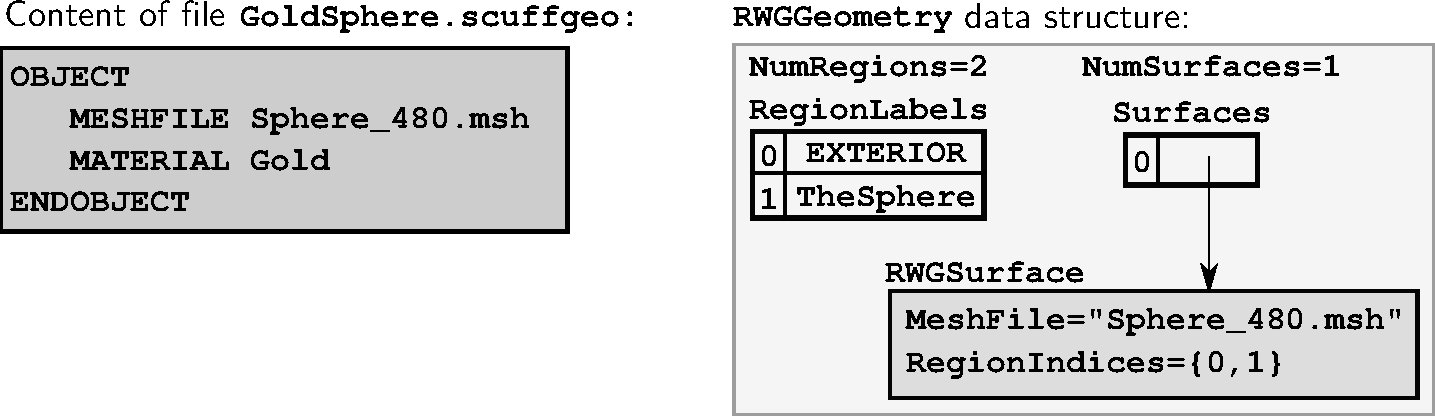
\includegraphics{RWGGeometryDataFields1.pdf}}
\caption{A simple \texttt{.scuffgeo} file and some fields in the 
         corresponding \texttt{RWGGeometry} structure.}
\end{center}
\end{figure}
%####################################################################%

In the language of regions and surfaces discussed above,
each \texttt{OBJECT} statement adds one new region and 
one new surface to a geometry. The newly added region 
is always taken to be the interior region associated
with the newly added surface, and corresponds to the
volume inside the object; the new surface exists at 
the interface between this region and the exterior
medium.

We said above that surface meshes for compact objects 
should be \textit{closed} surfaces. The exception to 
this statement is that PEC (perfectly electrically
conducting) or IPEC (imperfectly electrically 
conducting) bodies may be described by open surfaces.
(An IPEC body is a PEC body with finite surface 
conductivity). For both PEC and IPEC bodies the
interior fields vanish identically, and there
is no need for such bodies to have finite
interior volume. An \texttt{OBJECT} statement 
declaring a new PEC or IPEC object adds one new surface
but \textit{not} one new region to the geometry.

\subsection*{Simple geometries: Nested objects} 

It is possible for an object defined by an
\texttt{OBJECT} declaration to be fully 
contained inside another \texttt{OBJECT}. 
The nesting inclusion relationship is automatically 
detected by \ls. 

\subsection*{More complicated geometries: \texttt{REGION}
             and \texttt{SURFACE} statements}

Some geometries are too complicated to be defined 
as collections of compact objects bounded by closed 
surfaces. One example is a composite sphere in which 
the upper and lower hemispheres consist of different 
materials. Another example is a metallic nanoparticle 
(say, a disc) lying atop a dielectric substrate. The 
common feature of these two examples that prevents 
description in terms of simple closed objects is the 
presence of \textit{multi-material junctions}; these
are one-dimensional subspaces at which three
or more material regions meet. 
For the composite sphere, the multi-material junction 
would be the equator; for the disc on the substrate, 
it would be the lower circumference of the disc.

Geometries like this are described in \lss
using \texttt{REGION} and \texttt{SURFACE}
statements. For example, the composite sphere
above may be specified like this:
%####################################################################%
\begin{figure}[H]
\begin{center}
\resizebox{\textwidth}{!}{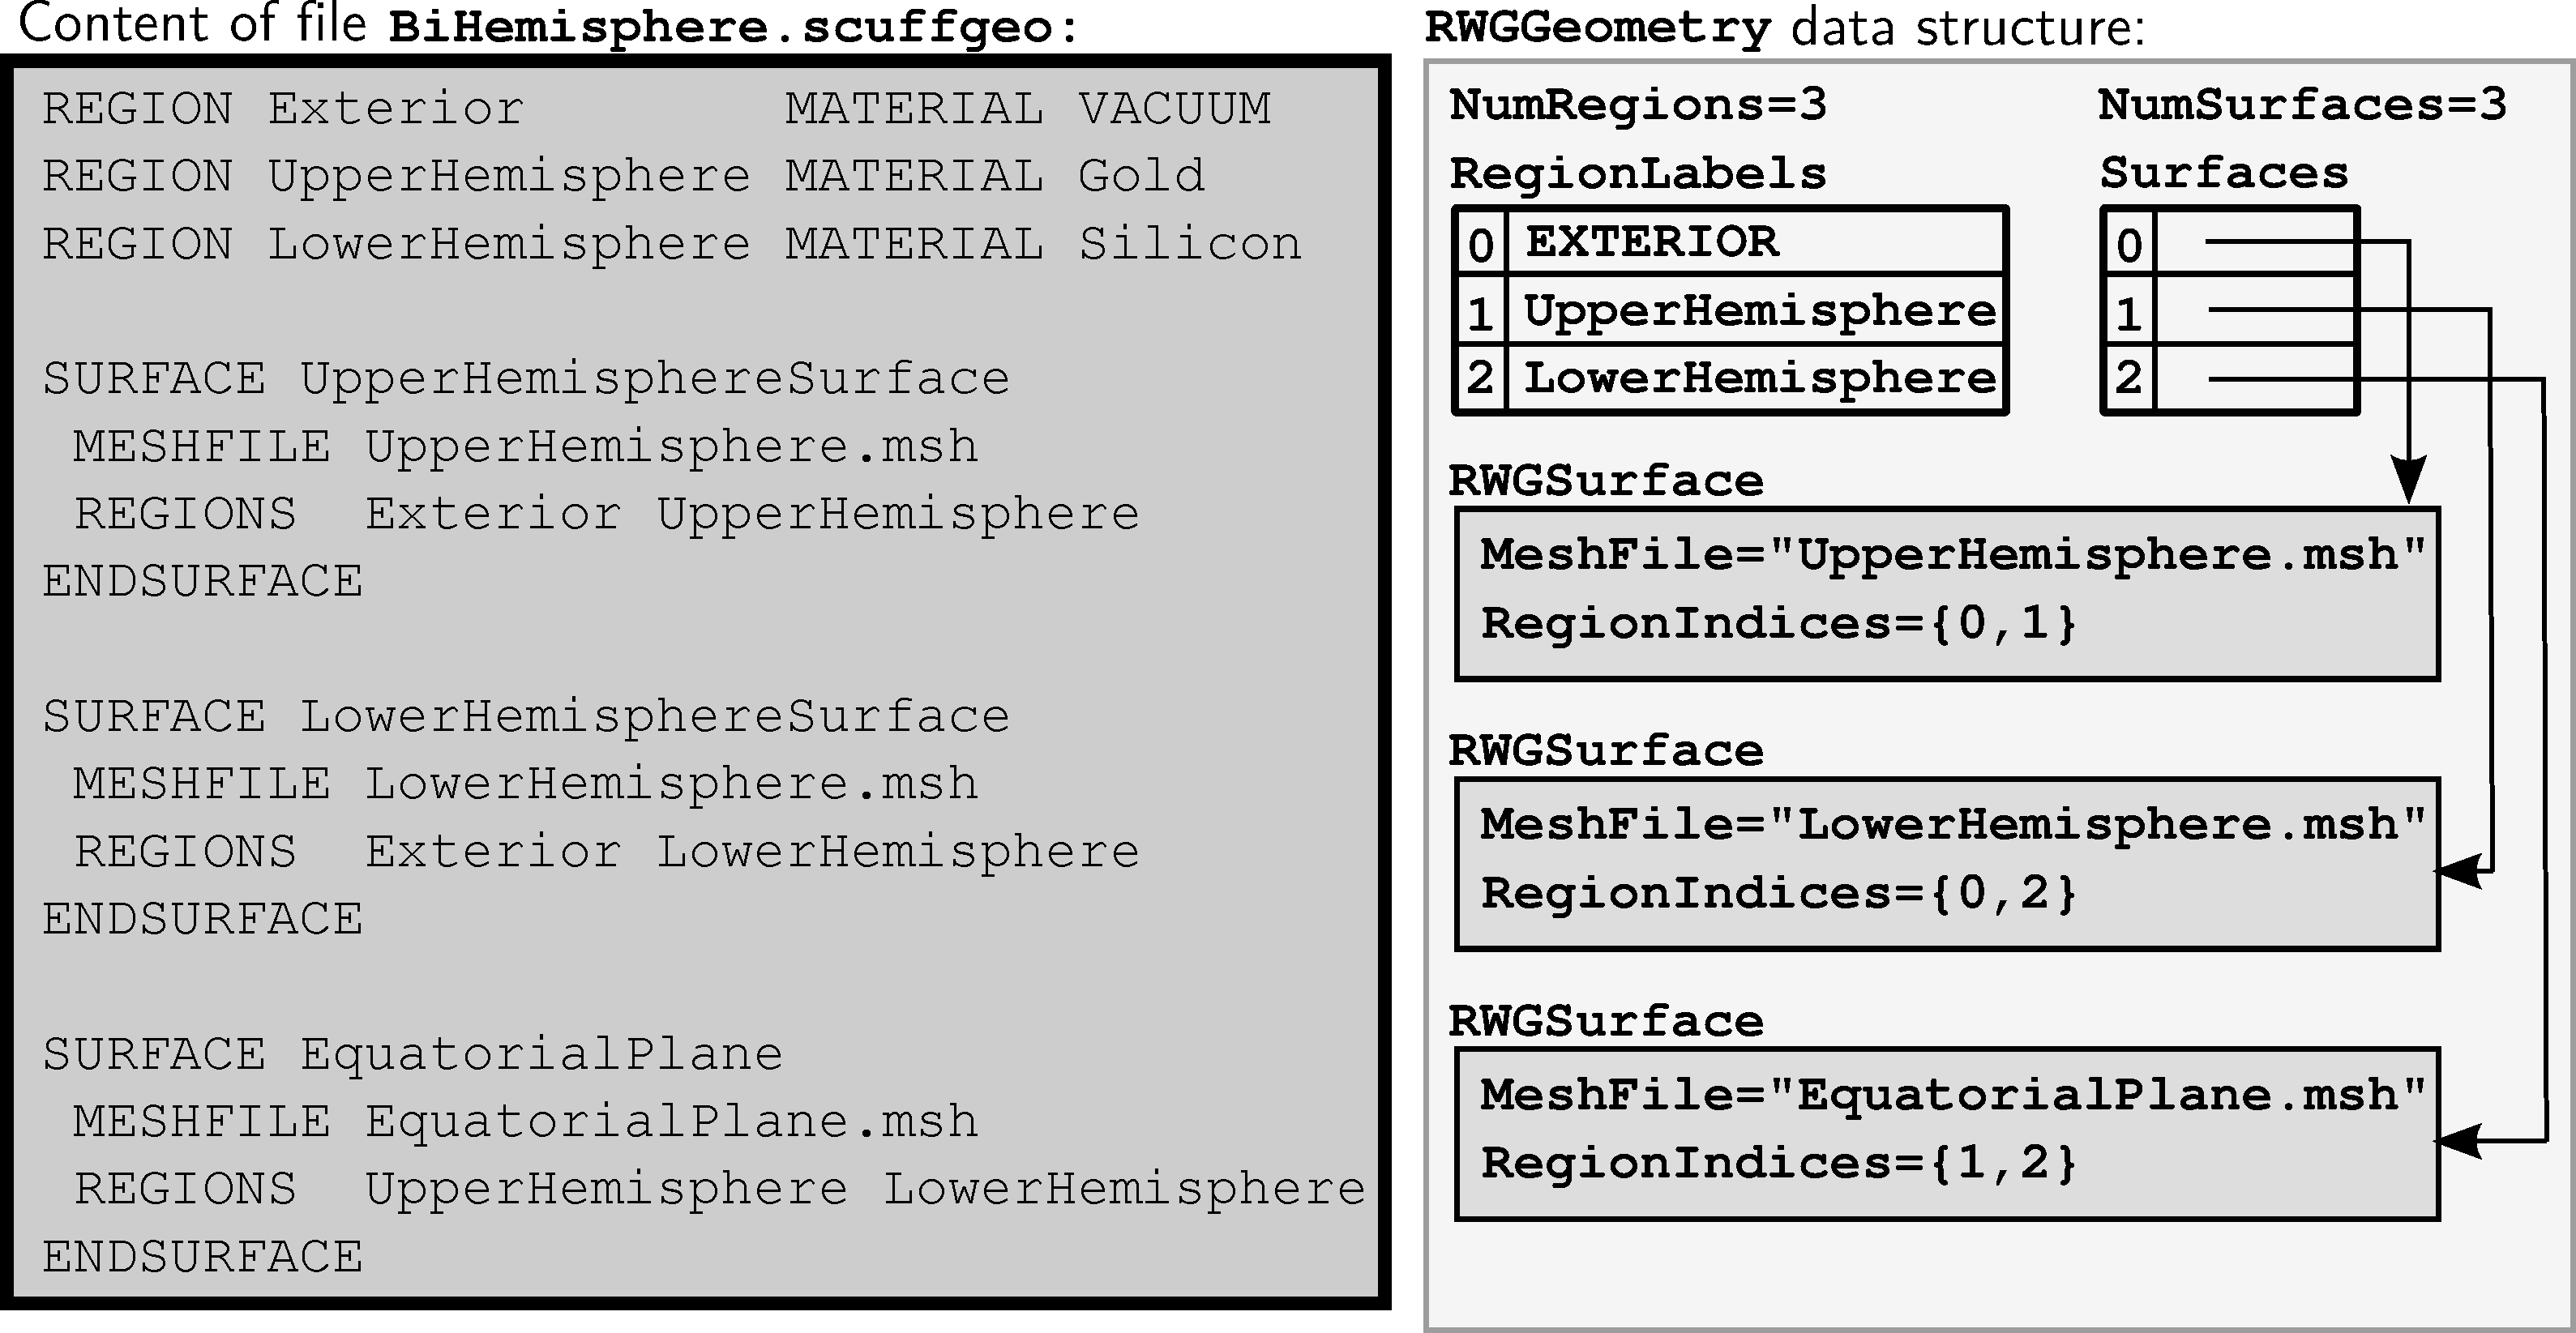
\includegraphics{RWGGeometryDataFields2.pdf}}
\caption{A more complex \texttt{.scuffgeo} file and some fields in the 
         corresponding \texttt{RWGGeometry} structure.}
\end{center}
\end{figure}
%####################################################################%
\subsection*{Extended geometries: \texttt{LATTICE}
             statements}

Extended geometries are described using \texttt{LATTICE}
statements in the \texttt{scuffgeo} file.
For example, here's an infinite square-lattice array 
of gold spheres:

\medskip

\begin{verbcode}
LATTICE
        VECTOR 1 0 
        VECTOR 0 1 
ENDLATTICE

OBJECT TheSphere
        MESHFILE Sphere_480.msh
        MATERIAL Gold
ENDOBJECT
\end{verbcode}

\medskip

It is also possible for surfaces to straddle 
the lattice-cell boundaries. This will be the 
case, for example, if you are describing an
infinite planar surface (possibly with
holes). In this case, the surface mesh must
be \textit{compatible} with the lattice specification,
in the sense that every triangle edge that 
lies on the unit-cell boundary must have an
image edge lying one lattice-translate away.

\subsection*{Extended geometries in which the exterior medium
             is non-contiguous}

In some extended geometries, it may be possible for the 
exterior medium to be non-contiguous. For example,
consider a thin film described by two planar surfaces  
(the upper and lower surfaces of the film) with a
\texttt{LATTICE} statement indicating the surfaces
are infinitely extended (comprised of an infinite
2D lattice of the unit-cell surfaces).
In this case, you probably think of the region above the 
upper surface and the region below the lower surface as 
both belonging to the same region, but as far as 
\lss is concerned they must be two different regions.

The reason for this is the following: Suppose both
the upper half-space and the lower half-space were
the same region (say \texttt{Exterior}). Then the upper 
and lower surfaces of the slab would both have 
\texttt{Exterior} as one of the two regions 
at whose interface they lie, and thus surface currents
on both the upper and lower surfaces would contribute 
to the scattered fields at all points in \texttt{Exterior}.
But this would be incorrect: Points in the upper half-space
receive scattered-field contributions only from currents
on the upper surface, while points in the lower half-space 
receive contributions only from the lower surface. 

The situation would be different if the upper and lower 
half-spaces were \textit{contiguous}---which would be
the case, for example, if the thin-film slab had a hole
in it. In this case, the upper and lower film surfaces
(as well as the hole sidewall surfaces) all form 
part of a single bounding surface separating the 
film interior from \texttt{Exterior}, and hence surface
currents on all of these surfaces contribute to the
scattered fields at points in \texttt{Exterior}.

%%%%%%%%%%%%%%%%%%%%%%%%%%%%%%%%%%%%%%%%%%%%%%%%%%%%%%%%%%%%%%%%%%%%%%
%%%%%%%%%%%%%%%%%%%%%%%%%%%%%%%%%%%%%%%%%%%%%%%%%%%%%%%%%%%%%%%%%%%%%%
%%%%%%%%%%%%%%%%%%%%%%%%%%%%%%%%%%%%%%%%%%%%%%%%%%%%%%%%%%%%%%%%%%%%%%
\newpage
\section{Representation of Surface Currents in \ls}

\subsection*{Surface Currents}

\lss is based on the surface-integral-equation approach
to computational electromagnetism. In this approach, the
fundamental unknowns are tangential \textit{surface
currents} flowing on the surfaces that lie at the 
interface between homogeneous material regions.

\subsubsection*{Electric and magnetic surface currents at dielectric 
                interfaces}
For the general case of a surface lying between two
dielectric regions, we have both an electric 
surface-current distribution $\vb K(\vb x)$ and a 
magnetic surface-current distribution $\vb N(\vb x)$
(here $\vb x$ is a point lying on the surface).
Both $\vb K$ and $\vb N$ are strictly \textit{tangential}
to the surface; they have no normal component.

\subsubsection*{Physical interpretation of surface currents}

One way to interpret the $\vb K$ and $\vb N$ currents
is as effective source distributions confined to the surfaces. 
In a real scattering problem involving dielectric bodies, the 
incident fields induce a physical volume electric current 
distribution $\vb J(\vb r)$ which is nonzero for all points 
$\vb r$ inside dielectric bodies, and the scattered fields 
are just the fields radiated by this source distribution.
The surface currents $\vb K$ and $\vb N$ are \textit{fictitious}
or (``effective'') source distributions with the property 
that the fields they radiate exactly reproduce the 
field radiated by the physical source distribution $\vb J$,
both inside and outside the body. What is unphysical about 
$\vb K$ and $\vb N$ is that \textbf{(a)} they are confined to 
the surfaces, whereas the physical induced source distribution
$\vb J$ exists throughout the volume, and \textbf{(b)} they
include magnetic currents $\vb N$, i.e. moving magnetic monopoles,
which do not actually exist in our universe.\footnote{Perhaps
we should say no more than \textit{one} of them exists in our 
universe: \url{http://prl.aps.org/abstract/PRL/v48/i20/p1378_1}.}
However, the fields radiated by $\vb K$ and $\vb N$ are 
perfectly physical.

Another, perhaps more direct, way to interpret the 
$\vb K$ and $\vb N$ currents is that they are nothing 
but rotated versions of the tangential components of 
the total electric and magnetic fields at the 
surface, i.e. we have 
$$ \vb K(\vb x) = \vbhat{n}\times \vb H\sups{tot}(\vb x), 
   \qquad 
   \vb N(\vb x) =-\vbhat{n}\times \vb E\sups{tot}(\vb x).
$$

\subsubsection*{Electric surface currents on PEC surfaces}

In the special case of a PEC surface---whether closed or
open---the magnetic surface current vanishes identically
($\vb N=0$) and only the electric surface current 
$\vb K$ is nonzero. In this case, the two interpretations of the 
surface currents discussed above coincide physically: 
Incident fields really do excite physical electric
currents on the surfaces of PEC bodies, these currents
really are strictly confined to the surfaces (in the
idealized limit of a \textit{perfect} electric conductor),
and the field radiated by these induced currents
really is the full scattered field.

\subsection*{RWG Basis Functions}
%####################################################################%
\begin{figure}
\begin{center}
\resizebox{\textwidth}{!}{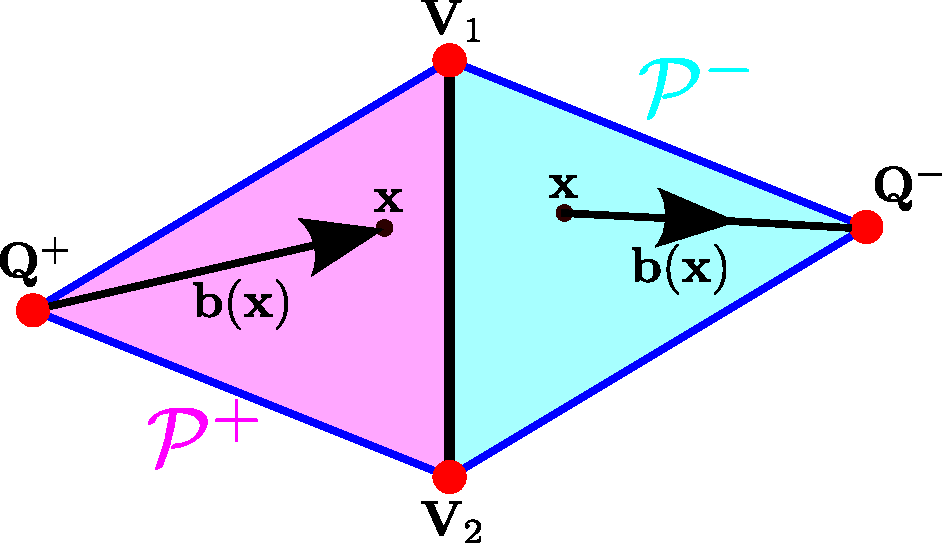
\includegraphics{RWGBasisFunctionNotation.pdf}}
\caption{Notation for RWG basis functions.}
\label{RWGNotationFigure}
\end{center}
\end{figure}
%####################################################################%

\lss uses RWG basis functions\footnote{S. M. Rao, D. R. Wilton, 
A. W. Glisson, \textit{IEEE Trans.\ Antennas Propagat.} 
\textbf{AP-30} 409 (1982).} to describe electric and magnetic 
surface currents flowing on the surfaces in a geometry. 
Each RWG basis function is assigned to a single interior
edge in a surface mesh discretization, and is nonvanishing
only on the two triangular panels that share that 
edge. 

To construct the RWG basis function associated with an 
edge (Figure \ref{RWGNotationFigure}), arbitrarily choose one 
of the two panels to be the \textit{positive} panel $\mc P^+$ 
associated with the basis function, while the other panel is the 
\textit{negative} panel $\mc P^-$. Let the vertices of the 
common edge be $\vb V_1$ and $\vb V_2$, and let the third vertex of 
$\mc P^+$ be the positive or \textit{source} vertex 
$\vb Q^+$ for the basis function, 
while the other opposite vertex will be the 
negative or \textit{sink} vertex $\vb Q^-$. Then 
the RWG basis function $\vb b(\vb x)$ associated with the
edge is defined as follows:
$$ \vb b(\vb x) = 
   \begin{cases}   
  +\frac{l}{2A^+}(\vb x - \vb Q^+), \qquad &\vb x \in \mc P^+ \\ 
  -\frac{l}{2A^+}(\vb x - \vb Q^-), \qquad &\vb x \in \mc P^- \\ 
   0, \qquad &\text{otherwise}
   \end{cases}
$$
where $l$ is the length of the common edge (the distance
$\vb V_1 \vb V_2$) and $\vb A^\pm$ are the areas of $\mc P^\pm$.
Thus the RWG function describes a current that emanates 
from $\vb Q^+$, grows linearly in strength as it flows along
the surface of $\mc P^+$ toward the common edge, begins
decreasing linearly in strength after crossing over that
edge into $\mc P^-$, and is sunk into $\vb Q^-$. There
is no current flow outside the pair of panels because
$\vb b(\vb x)$ has no component normal to any of the 
four exterior edges of the panel pair.

Figure \ref{RWGBasisFunctionFigure} illustrates some of the 
\lss data structures associated with a single RWG basis function
embedded in a surface mesh.
%####################################################################%
\begin{figure}
\begin{center}
\resizebox{\textwidth}{!}{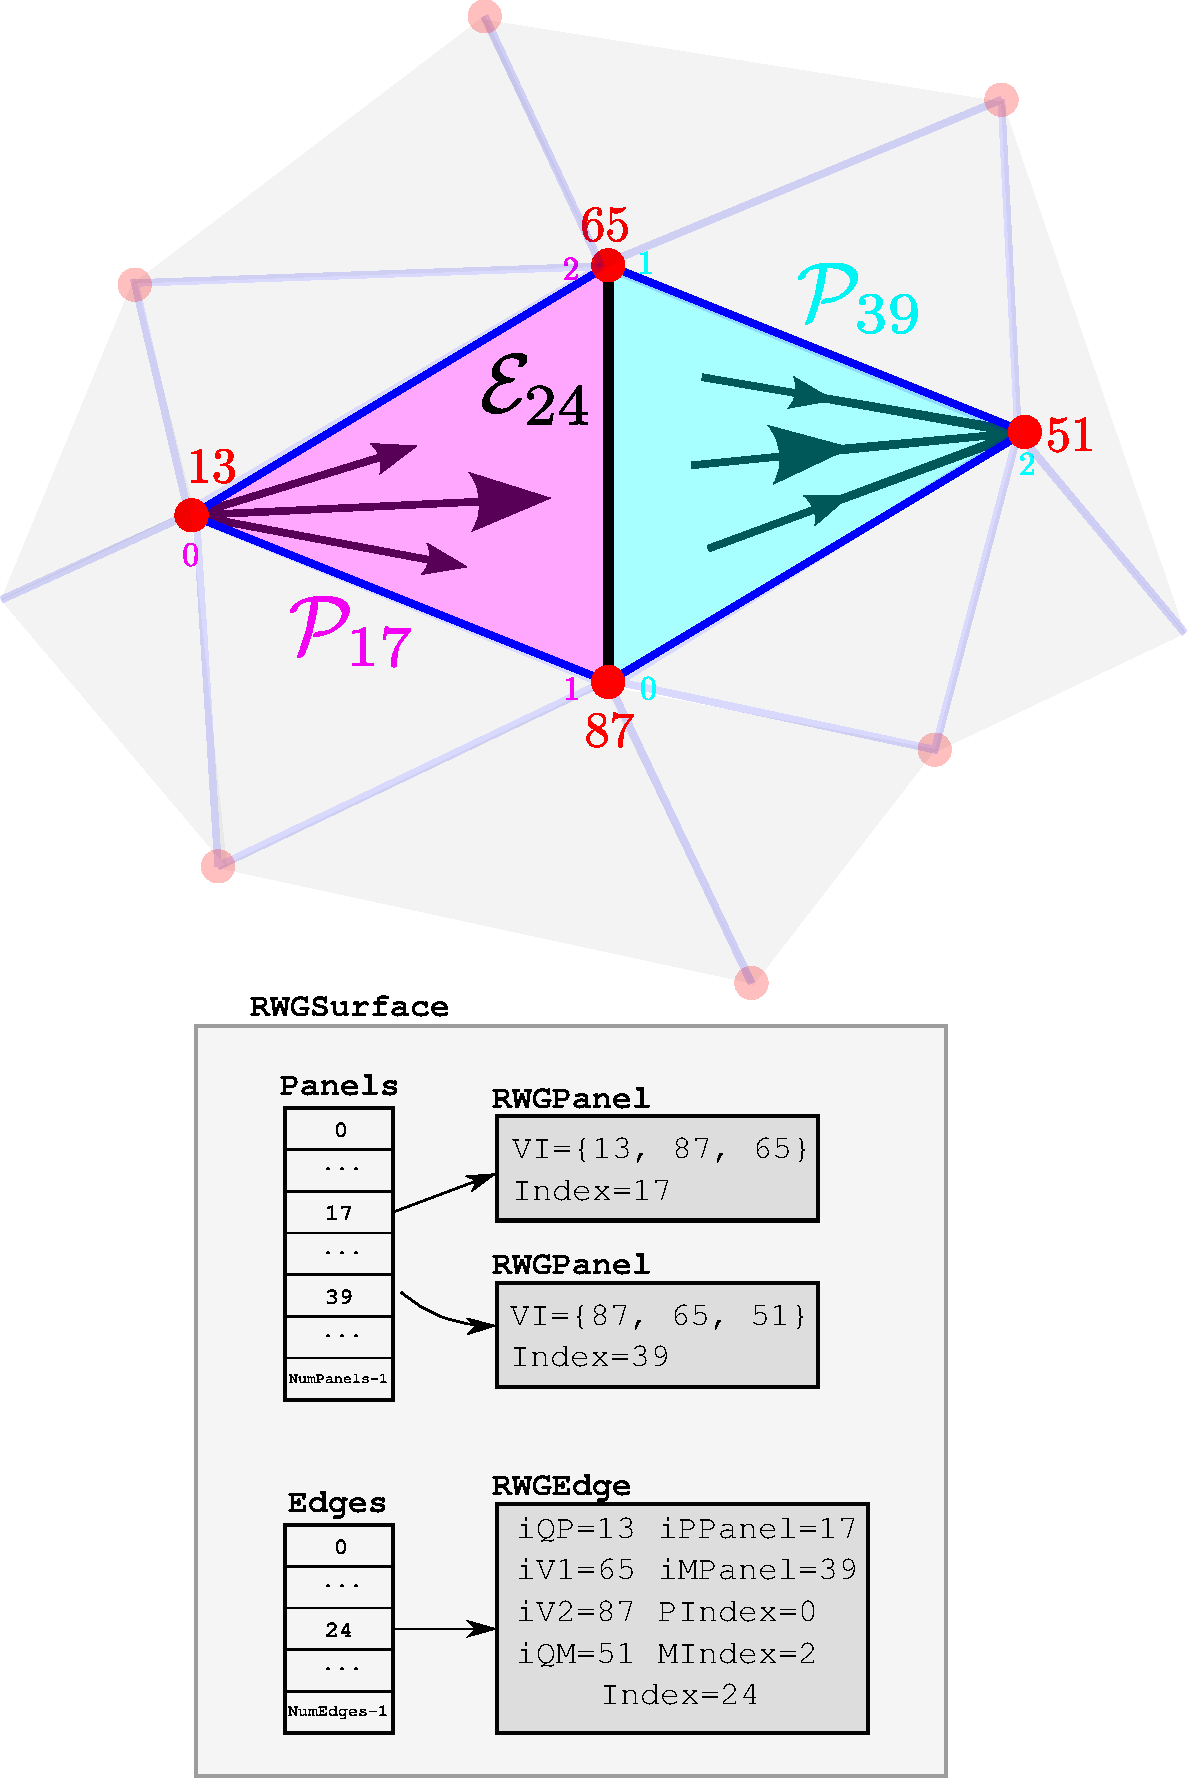
\includegraphics{RWGBasisFunction.pdf}}
\caption{A single RWG basis function associated with an internal edge 
         on an \texttt{RWGSurface}, and some portions of data structures 
         within the corresponding \texttt{RWGSurface} instance that 
         describe this basis function.}
\label{RWGBasisFunctionFigure}
\end{center}
\end{figure}
%####################################################################%

\subsection*{Half-RWG Basis Functions}

It is also possible to assign basis functions to 
\textit{exterior} edges of surface meshes, i.e.
edges that lie on the boundary of open surfaces.
In contrast to interior edges, exterior edges 
are associated within only one panel, not two
panels. {\sc scuff-em} adopts the convention
that this panel is the positive panel $\mc P^+$
for the edge, while there is no negative panel
$\mc P^-$. For exterior edges, the \texttt{iMPanel}
field of the \texttt{RWGEdge} structure 
is set to \texttt{-1}.



%%%%%%%%%%%%%%%%%%%%%%%%%%%%%%%%%%%%%%%%%%%%%%%%%%%%%%%%%%%%%%%%%%%%%%
%%%%%%%%%%%%%%%%%%%%%%%%%%%%%%%%%%%%%%%%%%%%%%%%%%%%%%%%%%%%%%%%%%%%%%
%%%%%%%%%%%%%%%%%%%%%%%%%%%%%%%%%%%%%%%%%%%%%%%%%%%%%%%%%%%%%%%%%%%%%%
\newpage
\section{Homogeneous Dyadic Green's Functions}
\label{DyadicGreensFunctionsSection}

Before proceeding, we must pause briefly to establish our 
conventions and notation for homogeneous dyadic Green's
functions.

Consider a spatial region characterized by spatially uniform 
relative permittivity and permeability $\epsilon^r$ and 
$\mu^r$. If we have
known distributions of electric and magnetic current
$\vb J(\vb x)$ and $\vb M(\vb x),$
we can compute the electric and magnetic fields in terms
of these currents and the properties of the medium, and  
the relevant convolution kernels in this procedure are
the dyadic Green's functions (DGFs):
%====================================================================%
\begin{align*}
 E_i(\vb x, \omega) 
&= 
   \int
    \Big\{
     \Gamma\supt{EE}_{ij}(\epsilon^r, \mu^r; \omega; \vb x, \vb x^\prime) 
     J_j(\vb x^\prime)
     +
     \Gamma\supt{EM}_{ij}(\epsilon^r, \mu^r; \omega; \vb x, \vb x^\prime) 
     M_j(\vb x^\prime)
    \Big\}
    \, d\vb x^\prime
\\
 H_i(\vb x, \omega) 
&= 
   \int
    \Big\{
     \Gamma\supt{ME}_{ij}(\epsilon^r, \mu^r; \omega; \vb x, \vb x^\prime) 
     J_j(\vb x^\prime)
     +
     \Gamma\supt{MM}_{ij}(\epsilon^r, \mu^r; \omega; \vb x, \vb x^\prime) 
     M_j(\vb x^\prime)
    \Big\}
    \, d\vb x^\prime.
\end{align*}
%====================================================================%

Explicit expressions for the DGFs are 
%====================================================================%
\begin{align*}
\BG\supt{EE}(\epsilon^r, \mu^r, \omega, \vb x, \vb x^\prime)
&=
 iZ_0 Z^r k^r \, \vb G(k^r, \vb x-\vb x^\prime)
\\[8pt]
%--------------------------------------------------------------------%
\BG\supt{ME}(\epsilon^r, \mu^r, \omega, \vb x, \vb x^\prime)
&=
 -ik^r \vb C(k^r, \vb x-\vb x^\prime)
\\[8pt]
%--------------------------------------------------------------------%
\BG\supt{EM}(\epsilon^r, \mu^r, \omega, \vb x, \vb x^\prime)
&=
 ik^r \, \vb C(k^r, \vb x-\vb x^\prime)
\\[8pt]
%--------------------------------------------------------------------%
\BG\supt{MM}(\epsilon^r, \mu^r, \omega, \vb x, \vb x^\prime)
&= \frac{ik^r}{Z_0 Z^r} \vb G(k^r, \vb x-\vb x^\prime)
\end{align*}
%====================================================================%
$$\bigg(Z_0=\sqrt\frac{\mu_0}{\epsilon_0},
        \qquad
        Z^r=\sqrt\frac{\mu^r}{\epsilon^r}, 
         \qquad
        k^r=\sqrt{\mu_0 \mu^r \epsilon_0 \epsilon^r}\cdot \omega
  \bigg)
$$
%====================================================================%
where $\vb G$, the ``photon Green's function,''
is the solution to the equation
\begin{equation}
 \Big[\nabla \times \nabla\times - \,\,k^2 \Big]\vb G(k; \vb r)
 =\delta(\vb r)\vb{1};
 \label{DyadicGFG}
\end{equation}
and $\vb C$ is defined by  
\begin{equation}
  \vb C(k, \vb r) = -\frac{1}{ik} \nabla \times \vb G(k, \vb r).
 \label{DyadicGFC}
\end{equation}
%
(Note that the $\BG$ dyadics depend separately on $\epsilon,\mu,$ 
and $\omega$, while $\vb G$ and $\vb C$ depend only on the 
combination $k=\sqrt{\epsilon\mu}\cdot \omega.$)

Explicit expressions for the components of $\vb G$ and $\vb C$ are 
\begin{align*}
G_{ij}(k,\vb r) 
 &= \frac{e^{ikr}}{4\pi (ik)^2 r^3}
    \bigg[ \Big(1-ikr + (ikr)^2 \Big)\delta_{ij}
          +\Big(-3 + 3ikr - (ikr)^2 \Big)\frac{r_i r_j}{r^2}
    \bigg]
\\
C_{ij}(k,\vb r) 
 &= \frac{e^{ikr}}{4\pi (ik) r^3} \varepsilon_{ijk} r_k 
    \Big(-1+ikr\Big)
\end{align*}
These may also be written in the form
\begin{equation}
G_{ij}(k,\vb r) =
  \Big[\delta_{ij} +\frac{1}{k^2} \partial_i \partial_j \Big]
  G_0(k, \vb r), \qquad
  C_{ij}(k, \vb r) = +\frac{1}{ik} \varepsilon_{ijl} 
                          \partial_l G_0(k, \vb r)
\label{GCfromG0}
\end{equation}
where $G_0$ is the scalar Green's function for the Helmholtz equation,
\numeq{ScalarGF}
{G_0(k; \vb r)
   =
  \frac{e^{ik|\vb r|}}{4\pi|\vb r|}
}
which satisfies
$$ \Big[ \nabla^2 + k^2 \Big] G_0(k; \vb r)
   =\delta(\vb r).
$$
With these expressions, we can verify that equation (\ref{DyadicGFC}) 
is actually just the first half of a pair of reciprocal curl identities 
relating $\vb G$ and $\vb C:$
\numeq{ReciprocalCurlIdentities}
{
  \frac{1}{ik} \nabla \times \vb G=-\vb C, 
\qquad
  \frac{1}{ik} \nabla \times \vb C=\vb G.
}
(As usual with tensors and dyadics, the vector notation here
is suggestive but vague; the precise meaning of (\ref{DyadicGFC}) is 
\numeq{ReciprocalCurlIdentities2}
{
   \frac{1}{ik} \varepsilon_{iAB} \partial_A G_{Bj} = -C_{ij},
   \qquad
   \frac{1}{ik} \varepsilon_{iAB} \partial_A C_{Bj} = G_{ij}.)
}


%%%%%%%%%%%%%%%%%%%%%%%%%%%%%%%%%%%%%%%%%%%%%%%%%%%%%%%%%%%%%%%%%%%%%%
%%%%%%%%%%%%%%%%%%%%%%%%%%%%%%%%%%%%%%%%%%%%%%%%%%%%%%%%%%%%%%%%%%%%%%
%%%%%%%%%%%%%%%%%%%%%%%%%%%%%%%%%%%%%%%%%%%%%%%%%%%%%%%%%%%%%%%%%%%%%%

\paragraph{Shorthand} In what follows, an equation like 

$$ E_i(\vb x, \omega) = 
   \int_{\mathcal S} 
     \Gamma\supt{EE}_{ij}(\epsilon^r, \mu^r; \omega; 
                          \vb x, \vb x^\prime) 
     K_j(\vb x^\prime)
    \, d\vb x^\prime
$$
will often be abbreviated to read 
$$ \vb E(\vb x) = 
    \int_{\mathcal S} 
      \BG\supt{EE}(\mathcal{R}^r; \vb x, \vb x^\prime) 
         \cdot \vb K(\vb x^\prime) 
    \, d\vb x^\prime
$$
(with $\omega$ arguments suppressed and the dependence 
on $\epsilon^r, \mu^r$ condensed into a dependence
on the region $\mathcal{R}^r$), or even abbreviated further
to read
$$ \vb E = \BG\supt{EE}(\mathcal{R}^r) \star \vb K $$
where $\star$ denotes a convolution operation.


\include{lsInnardsSections/FieldsOfIndividualBFs}
%%%%%%%%%%%%%%%%%%%%%%%%%%%%%%%%%%%%%%%%%%%%%%%%%%%%%%%%%%%%%%%%%%%%%%
%%%%%%%%%%%%%%%%%%%%%%%%%%%%%%%%%%%%%%%%%%%%%%%%%%%%%%%%%%%%%%%%%%%%%%
%%%%%%%%%%%%%%%%%%%%%%%%%%%%%%%%%%%%%%%%%%%%%%%%%%%%%%%%%%%%%%%%%%%%%%
\newpage
\section{Computation of the fields in \lss geometries}

Using the fields of individual basis functions as
discussed in the previous section, we can compute the 
total $\vb E$ and $\vb H$ fields at arbitrary points 
in a {\sc scuff-em} geometry.


\subsection{The simplest case}

The simplest case to consider is that in which we have
a single compact body $\mc B$ in vacuum; let the body surface
be $\mc S=\partial \mc B$ and suppose the incident fields 
arise from sources lying outside $\mc B$. Let the surface-current
coefficients be $\{\vb k_\alpha, \vb n_\alpha\}$, so that 
the electric and magnetic surface currents are
%====================================================================%
$$ \vb K(\vb x) = \sum_{\alpha} k_\alpha \vb b_\alpha(\vb x),
   \qquad
   \vb N(\vb x) = \sum_{\alpha} n_\alpha \vb b_\alpha(\vb x)
$$
%====================================================================%
where $\{\vb b_\alpha\}$ is the set of RWG basis functions 
on surface $\partial \mc B$. Then the fields at a point outside 
$\mc B$ are
%====================================================================%
\begin{subequations}
\begin{align}
 \vb E(\vb x) 
  &= \vb E\sups{inc}(\vb x) + 
\sum_{\alpha} \Big\{ ik_0Z_0 k_\alpha \vb e_\alpha(k_0; \vb x)
                             -n_\alpha \vb h_\alpha(k_0; \vb x)
                   \Big\}
\\
 \vb H(\vb x) 
  &= \vb H\sups{inc}(\vb x) + 
     \sum_{\alpha} \Big\{     k_\alpha \vb h_\alpha(k_0; \vb x)
                         +\frac{ik_0}{Z_0} n_\alpha \vb e_\alpha(k_0; \vb x)
                   \Big\}.
\end{align}
\label{OutsideFields}
\end{subequations}
%====================================================================%
The fields at a point inside $\mc B$ are 
%====================================================================%
\begin{subequations}
\begin{align}
 \vb E(\vb x)
  &= -\sum_{\alpha} \Big\{ ik_1Z_1 k_\alpha \vb e_\alpha(k_1; \vb x)
                                  -n_\alpha \vb h_\alpha(k_1; \vb x)
                   \Big\}
\\
 \vb H(\vb x) 
  &= -\sum_{\alpha} \Big\{     k_\alpha \vb h_\alpha(k_1; \vb x)
                         +\frac{ik_1}{Z_1} n_\alpha \vb e_\alpha(k_1; \vb x)
                   \Big\}.
\end{align}
\label{InsideFields}
\end{subequations}
%====================================================================%
Note the following differences between (\ref{OutsideFields}) and
(\ref{InsideFields}):
\begin{itemize}
 \item The incident fields contribute to (\ref{OutsideFields})
       but not to (\ref{InsideFields}).
 \item Equation (\ref{InsideFields}) involves a minus sign that 
       is not present in (\ref{OutsideFields}).
 \item Equation (\ref{OutsideFields}) involves the vacuum
       wavenumber $k_0=\omega/c$ and the vacuum 
       wave impedance $Z_0\approx 377 \, \Omega.$
       Equation (\ref{InsideFields}) involves the wavenumber 
       $k_1=\sqrt{\epsilon^r \mu^r}k_0$ and wave impedance 
       $Z_1=\sqrt{\frac{\mu^r}{\epsilon^r}}Z_0$ for the body interior.
       (Here $\{\epsilon^r, \mu^r\}$ are the relative permittivity 
        and permeability of the medium inside body $\mc B$ at the 
        frequency in question.)
\end{itemize}

\subsection{The general case}

The previous discussion was for the simplest case of a 
single compact body in vacuum with incident-field 
sources lying outside the body. The generalization
to more complicated cases is straighforward. 

Consider a point $\vb x$ in some region $\mathcal{R}$
of a \lss geometry. In general, $\mathcal{R}$
will be bounded by some collection of surfaces
$\{\mathcal{S}^s\}$. Let's subdivide the set of 
surfaces bounding $\mathcal{R}$ into two groups:
a first set $\{\mathcal{S}^\alpha\}$ for which
$\mathcal{R}$ is the \textit{exterior} surface,
and a second set $\{\mathcal{S}^\beta\}$ for which
$\mathcal{R}$ is the \textit{interior} surface.
Then the electric field at $\vb x$ is
%====================================================================%
\begin{align} 
E_i(\vb x) 
    = &\hphantom{-} \sum_\alpha \int_{\mathcal{S}^\alpha} 
           \Big\{ \Gamma_{ij}\supt{EE}(\mathcal{R}; \vb x, \vb x^\prime) 
                   K_j(\vb x^\prime)
                  \,+\,
                   \Gamma_{ij}\supt{EM}(\mathcal{R}; \vb x, \vb x^\prime) 
                   N_j(\vb x^\prime)
           \Big\} \, d\vb x^\prime
\nn
     &-\sum_\beta \int_{\mathcal{S}^\beta} 
           \Big\{ \Gamma_{ij}\supt{EE}(\mathcal{R}; \vb x, \vb x^\prime) 
                   K_j(\vb x^\prime)
                  \,+\,
                   \Gamma_{ij}\supt{EM}(\mathcal{R}; \vb x, \vb x^\prime) 
                   N_j(\vb x^\prime)
           \Big\} \, d\vb x^\prime
\nn
     &+E^{\text{\scriptsize inc},r}_i(\vb x).
\label{FieldContributionsEquation}
\end{align}
%====================================================================%
In this equation, $\vb E\incr$ is the field due to any 
incident field sources that lie inside the region $\mathcal{R}^r.$
(The $\vb H$ fields are given by identical relations with 
$\{ \Gamma\supt{EE}, \Gamma\supt{EM}, E\incr\} \to 
 \{ \Gamma\supt{ME}, \Gamma\supt{MM}, H\incr\}$.)

Note the following points with respect to equation
(\ref{FieldContributionsEquation}):
\begin{itemize}
  \item Sources on surfaces $\mathcal{S}_\alpha$ for which
        $\mathcal{R}$ is the exterior medium  
        contribute to the fields at $\vb x$ 
        with a positive sign.
        Sources on surfaces $\mathcal{S}_\beta$ for which
        $\mathcal{R}$ is the interior medium  
        contribute to the fields at $\vb x$ 
        with a negative sign.

  \item In each line of (\ref{FieldContributionsEquation}), 
        (i.e. regardless of the surface over which we are 
        integrating) the Green's functions used to compute
        the fields at $\vb x$ are the Green's functions for
        the homogeneous region $\mathcal{R}$ containing $\vb x$.
        The material properties of other regions are not
        referenced.
\end{itemize}

%####################################################################%
%####################################################################%
%####################################################################%
\begin{figure}
\begin{center}
%\includegraphics{FieldContributionsFigure}
\caption{Contributions of objects to the scattered fields at 
         an arbitrary point $\vb x$. Objects $\mathcal{O}_\beta$
         and $\mathcal{O}_\gamma$ contribute
         to the field at $\vb x$ ``with a plus sign'' 
         (cf. equation \ref{FieldContributionsEquation}).
         Object $\mathcal{O}_\alpha$ 
         contributes to the field at $\vb x$ ``with a minus
         sign.'' Objects $\mathcal{O}_\delta$ and $\mathcal{O}_\lambda$
         do not contribute to the field at $\vb x$.}
\label{FieldContributionsFigure}
\end{center}
\end{figure}

\documentclass[letterpaper]{article}

%********************************************************
%* latex shortcuts used for libscuff documentation files
%* 
%* homer reid -- 1994--2011
%**************************************************
\usepackage{graphicx}
\usepackage{color}
\usepackage{dsfont}
\usepackage{bbm}
\usepackage{amsmath}
\usepackage{amssymb}
\usepackage{float}
\usepackage{psfrag}
\usepackage{mathdots}
%\usepackage{algorithm}
%\usepackage{algorithmic}
%\usepackage{listings}
\usepackage{array}
\usepackage{url}
\usepackage{arydshln}
\usepackage{fancybox}
\usepackage{fancyvrb}
\usepackage{verbatim}

%--------------------------------------------------
%- boldface greek letters 
%--------------------------------------------------
\newcommand\vbphi{\mathbf{\phi}}
\newcommand\vbPhi{\mathbf{\Phi}}
\newcommand{\vbDelta}{\boldsymbol{\Delta}}
\newcommand{\vbrho}{\boldsymbol{\rho}}
\newcommand{\vbchi}{\boldsymbol{\chi}}

%--------------------------------------------------
%- colors -----------------------------------------
%--------------------------------------------------
\newcommand{\red}[1]{\textcolor{red}{#1}}
\newcommand{\blue}[1]{\textcolor{blue}{#1}}
\newcommand{\green}[1]{\textcolor{green}{#1}}
\newcommand{\atan}{\text{atan}}

%--------------------------------------------------
% general commands
%--------------------------------------------------
\newcommand\Tr{\hbox{Tr }}
\newcommand\sups[1]{^{\hbox{\scriptsize{#1}}}}
\newcommand\supt[1]{^{\hbox{\tiny{#1}}}}
\newcommand\subs[1]{_{\hbox{\scriptsize{#1}}}}
\newcommand\subt[1]{_{\hbox{\tiny{#1}}}}
\newcommand{\nn}{\nonumber \\}
\newcommand{\vb}[1]{\mathbf{#1}}
\newcommand{\numeq}[2]{\begin{equation} #2 \label{#1} \end{equation}}
\newcommand{\pard}[2]{\frac{\partial #1}{\partial #2}}
\newcommand{\pardn}[3]{\frac{\partial^{#1} #2}{\partial #3^{#1}}}
\newcommand{\pf}[2]{\left(\frac{#1}{#2}\right)}
\newcommand{\pp}{{\prime\prime}}
\newcommand{\vbhat}[1]{\vb{\hat #1}}
\newcommand{\mc}[1]{\mathcal{#1}}
\newcommand{\bmc}[1]{\boldsymbol{\mathcal{#1}}}
\newcommand{\mb}[1]{\mathbb{#1}}
\newcommand{\ds}[1]{\displaystyle{#1}}
\newcommand{\primedsum}{\sideset{}{'}{\sum}}
\newcommand{\pan}{\mathcal{P}}

%--------------------------------------------------
%- special libscuff stuff--------------------------
%--------------------------------------------------
\newcommand\ls{{\sc libscuff}}
\newcommand\lss{{\sc libscuff\,}}
\newcommand{\BG}{\boldsymbol{\Gamma}}
\newcommand{\MInt}{\vb{\hat M}}
\newcommand{\NInt}{\vb{\hat N}}
\newcommand{\MExt}{\vb{\check M}}
\newcommand{\NExt}{\vb{\check N}}
\newcommand{\xInt}{\vb{\hat x}}
\newcommand{\xExt}{\vb{\check x}}

%--------------------------------------------------
%-- superscripts for dyadic green's functions 
%--------------------------------------------------
\newcommand{\EEe}{^{\hbox{\tiny{EE}\scriptsize{,$e$}}}}
\newcommand{\MEe}{^{\hbox{\tiny{ME}\scriptsize{,$e$}}}}
\newcommand{\EMe}{^{\hbox{\tiny{EM}\scriptsize{,$e$}}}}
\newcommand{\MMe}{^{\hbox{\tiny{MM}\scriptsize{,$e$}}}}
\newcommand{\EEr}{^{\hbox{\tiny{EE}\scriptsize{,$r$}}}}
\newcommand{\MEr}{^{\hbox{\tiny{ME}\scriptsize{,$r$}}}}
\newcommand{\EMr}{^{\hbox{\tiny{EM}\scriptsize{,$r$}}}}
\newcommand{\MMr}{^{\hbox{\tiny{MM}\scriptsize{,$r$}}}}
\newcommand{\incr}{^{\text{\scriptsize inc},r}}
\newcommand{\incro}{^{\text{\scriptsize inc},r_1}}
\newcommand{\incrt}{^{\text{\scriptsize inc},r_2}}

%%%%%%%%%%%%%%%%%%%%%%%%%%%%%%%%%%%%%%%%%%%%%%%%%%%%%%%%%%%%%%%%%%%%%%
%%%%%%%%%%%%%%%%%%%%%%%%%%%%%%%%%%%%%%%%%%%%%%%%%%%%%%%%%%%%%%%%%%%%%%
%%%%%%%%%%%%%%%%%%%%%%%%%%%%%%%%%%%%%%%%%%%%%%%%%%%%%%%%%%%%%%%%%%%%%%
\newcommand{\MMExt}{\check{\mathcal{M}}}
\newcommand{\MMInt}{\hat{\mathcal{M}}}
\newcommand{\NNExt}{\check{\mathcal{N}}}
\newcommand{\NNInt}{\hat{\mathcal{N}}}
\newcommand{\BMMExt}{\boldsymbol{\check{\mathcal{M}}}}
\newcommand{\BMMInt}{\boldsymbol{\hat{\mathcal{M}}}}
\newcommand{\BNNExt}{\boldsymbol{\check{\mathcal{N}}}}
\newcommand{\BNNInt}{\boldsymbol{\hat{\mathcal{N}}}}
\newpage

%--------------------------------------------------
%- inner products and operator matrix elements  ---
%--------------------------------------------------
\newcommand{\expval}[1]{ \big\langle #1 \big\rangle}
\newcommand{\Expval}[1]{ \Big\langle #1 \Big\rangle}
\newcommand{\inp}[2]{ \big\langle #1 \big| #2 \big\rangle}
\newcommand{\Inp}[2]{ \Big\langle #1 \Big| #2 \Big\rangle}
\newcommand{\INP}[2]{ \bigg\langle #1 \bigg| #2 \Big\rangle}
\newcommand{\vmv}[3]{ \big\langle #1 \big| #2 \big| #3 \big\rangle}
\newcommand{\VMV}[3]{ \Big\langle #1 \Big| #2 \Big| #3 \Big\rangle}

%------------------------------------------------------------
%- shaded box for source code inclusions 
%------------------------------------------------------------
%\definecolor{lightgrey}{rgb}{0.85,0.85,0.85}
%\newcommand{\SourceBox}[1]
% { \begin{mdframed}[backgroundcolor=lightgrey, linewidth=2pt,
%                    tikzsetting={draw=black, line width=2pt,
%                                 dashed, dash pattern= on 5pt off 5pt}] %
%  \begin{verbatim} #1 \end{verbatim} \end{mdframed} \medskip
%}
%\IfFileExists{mdframed.sty}
% { \usepackage{mdframed}
%   \surroundwithmdframed[backgroundcolor=lightgrey, linewidth=2pt,
%                         framemethod=tikz,
%                         skipabove=10pt,
%                         skipbelow=10pt,
%                         tikzsetting={draw=black, line width=2pt,
%                                      dashed, dash pattern= on 5pt off 5pt}
%                        ]{verbatim}
% }
% {
% }
%--------------------------------------------------
%- shaded verbatim for code inclusions
%--------------------------------------------------
\definecolor{lightgrey}{rgb}{0.85,0.85,0.85}
\newenvironment{verbcode}{\VerbatimEnvironment% 
  \noindent
  %{\columnwidth-\leftmargin-\rightmargin-2\fboxsep-2\fboxrule-4pt} 
  \begin{Sbox} 
  \begin{minipage}{\linewidth}
  \begin{Verbatim}
}{% 
  \end{Verbatim}  
   \end{minipage}
  \end{Sbox} 
  \fcolorbox{black}{lightgrey}{\textcolor{black}{\TheSbox}}
} 


\graphicspath{{figures/}}

%------------------------------------------------------------
%------------------------------------------------------------
%- Special commands for this document -----------------------
%------------------------------------------------------------
%------------------------------------------------------------$
\newcommand{\FSV}{\boldsymbol{\mathcal{F}}}   % field six-vector
\newcommand{\CSV}{\boldsymbol{\mathcal{C}}}   % current six-vector
\newcommand{\BSV}{\boldsymbol{\mathcal{B}}}   % basis-function six-vector
\newcommand{\SSV}{\boldsymbol{\mathcal{S}}}   % source six-vector

\newcommand{\NM}{\boldsymbol{\mathcal{N}}}
\newcommand{\SVDGF}{\boldsymbol{\mathcal{G}}} % six-vector DGF

\newcommand{\SVChi}{\boldsymbol{\chi}}        % six-vector susceptibility

%------------------------------------------------------------
%------------------------------------------------------------
%- Document header  -----------------------------------------
%------------------------------------------------------------
%------------------------------------------------------------
\title {SIE-BEM Formulations in {\sc scuff-em}}
\author {Homer Reid}
\date {March 29, 2013}

%------------------------------------------------------------
%------------------------------------------------------------
%- Start of actual document
%------------------------------------------------------------
%------------------------------------------------------------

\begin{document}
\pagestyle{myheadings}
\markright{Homer Reid: SIE-BEM Formulations in {\sc scuff-em}}
\maketitle

\tableofcontents

Consider a single dielectric object in a medium.   
I define $\vbhat{n}$ to be the outward pointing normal vector
and $\{\vb K, \vb N\}=
\{\vbhat{n}\times \vb H\sups{tot}, -\vbhat{n}\times\vb E\sups{tot}\}$
to be the surface currents seen from the exterior medium.
The quantities $\vbhat{n}, \vb{K}, \vb{N}$ all suffer a sign flip
when reckoned from the interior medium; I will not define
separate notation for the sign-flipped version of these
quantities.

Six-vector notation for fields, surface currents, and dyadic Green's
functions:
$$ \FSV=\left(\begin{array}{c} \vb E \\ \vb H \end{array}\right), \qquad
   \CSV=\left(\begin{array}{c} \vb K \\ \vb N \end{array}\right), \qquad
   \SVDGF=\left(\begin{array}{cc} 
      \BG\supt{EE} & \BG\supt{EM}  \\
      \BG\supt{ME} & \BG\supt{MM} 
          \end{array}\right).
$$
The total fields in the exterior and interior regions are related
to the surface currents and the incident fields (which we assume
to arise from sources in the exterior medium) according to
\begin{subequations}
\begin{align}
 \FSV\subs{ext}\sups{tot} &= \SVDGF\subs{ext} * \CSV + \FSV\sups{inc} \\
 \FSV\subs{int}\sups{tot} &= -\SVDGF\subs{int} * \CSV
\end{align}
\label{FGC}
\end{subequations}
On the other hand, the surface currents are related to the 
total fields in the two regions according to
\begin{subequations}
\begin{align}
 \CSV &=  \NM\FSV\sups{tot}\subs{ext}
\\
 \CSV &= -\NM\FSV\sups{tot}\subs{int}
\intertext{where}
 \NM &=
   \left(\begin{array}{cc} 
   0               & \vbhat{n}\times \\
  -\vbhat{n}\times & 0
   \end{array} \right).
\end{align}
\label{CNF}
\end{subequations}
%
Combining (\ref{CNF}) with (\ref{FGC}) yields 
two distinct six-vector integral equations
relating $\CSV$ to $\FSV\sups{inc}$:
\begin{subequations}
\begin{align}
\end{align}
\end{subequations}


\footnote{This way of understanding the PMCHW and n-Muller
formulations follows P. Yla-Oijala and M. Taskinen,
``Well-conditioned Muller formulation for electromagnetic 
scattering by dielectric objects,'' \textit{IEEE Transactions 
on Antennas and Propagation}, \textbf{53} 3316 (2005).}

%%%%%%%%%%%%%%%%%%%%%%%%%%%%%%%%%%%%%%%%%%%%%%%%%%%%%%%%%%%%%%%%%%%%%%
%%%%%%%%%%%%%%%%%%%%%%%%%%%%%%%%%%%%%%%%%%%%%%%%%%%%%%%%%%%%%%%%%%%%%%
%%%%%%%%%%%%%%%%%%%%%%%%%%%%%%%%%%%%%%%%%%%%%%%%%%%%%%%%%%%%%%%%%%%%%%
\newpage
\end{document}

@ARTICLE{Helsinki2005,
author={Yla-Oijala, P. and Taskinen, M.}, 
journal={Antennas and Propagation, IEEE Transactions on}, 
title={Well-conditioned Muller formulation for electromagnetic scattering by dielectric objects}, 
year={2005}, 
volume={53}, 
number={10}, 
pages={3316-3323}, 
keywords={Galerkin method;dielectric bodies;electric breakdown;electric field integral equations;electromagnetic wave scattering;iterative methods;magnetic field integral equations;matrix algebra;method of moments;surface electromagnetic waves;Galerkin method;MoM;N-Muller;RWG basis function;Rao-Wilton-Glisson;electromagnetic scattering;electrostatic integral equation;homogeneous dielectric object;iterative solution;low-frequency breakdown;magnetostatic integral equation;method of moments;surface integral equation;well-conditioned Muller formulation;well-conditioned matrix equation;Dielectric breakdown;Electric breakdown;Electromagnetic scattering;Electrostatics;Helium;Integral equations;Iterative methods;Magnetostatic waves;Microwave frequencies;Moment methods;Dielectric object;MÜller formulation;electromagnetic scattering;low frequency;method of moments (MoM);surface integral equation}, 
doi={10.1109/TAP.2005.856313}, 
ISSN={0018-926X},}

%%%%%%%%%%%%%%%%%%%%%%%%%%%%%%%%%%%%%%%%%%%%%%%%%%%%%%%%%%%%%%%%%%%%%%
%%%%%%%%%%%%%%%%%%%%%%%%%%%%%%%%%%%%%%%%%%%%%%%%%%%%%%%%%%%%%%%%%%%%%%
%%%%%%%%%%%%%%%%%%%%%%%%%%%%%%%%%%%%%%%%%%%%%%%%%%%%%%%%%%%%%%%%%%%%%%
\newpage
\section{Evaluation of 2D Integrals over RWG Basis Functions}

The $\vb E$ and $\vb H$ fields due to an electric current distribution
described by a single unit-strength RWG basis function $\vb f_a(\vb x)$ 
are 
%--------------------------------------------------------------------%
\begin{align}
  \vb E(\vb x) &= ikZ \INP{\vb G(\vb x, \vb x^\prime)}{\vb f_a(\vb x^\prime)}\\
  \vb H(\vb x) &= -ik \INP{\vb C(\vb x, \vb x^\prime)}{\vb f_a(\vb x^\prime)}.
\end{align}
%--------------------------------------------------------------------%
The fields of a \textit{magnetic} current distribution
described by the same basis function are 
%--------------------------------------------------------------------%
\begin{align}
  \vb E(\vb x) &= +ik \INP{\vb C(\vb x, \vb x^\prime)}{\vb f_a(\vb x^\prime)}\\
  \vb H(\vb x) &= \frac{ik}{Z} \INP{\vb C(\vb x, \vb x^\prime)}{\vb f_a(\vb x^\prime)}.
\end{align}
%--------------------------------------------------------------------%

%%%%%%%%%%%%%%%%%%%%%%%%%%%%%%%%%%%%%%%%%%%%%%%%%%%%%%%%%%%%%%%%%%%%%%
%%%%%%%%%%%%%%%%%%%%%%%%%%%%%%%%%%%%%%%%%%%%%%%%%%%%%%%%%%%%%%%%%%%%%%
%%%%%%%%%%%%%%%%%%%%%%%%%%%%%%%%%%%%%%%%%%%%%%%%%%%%%%%%%%%%%%%%%%%%%%
\newpage
\section{Evaluation of 4D Integrals over RWG Basis Functions}

As demonstrated above, the elements of the BEM matrix involve
integrals over pairs of RWG basis functions of the form
%====================================================================%
\begin{subequations}
\begin{align}
 \Big\langle \vb f_a \Big| \vb G(k) \Big | \vb f_b \Big \rangle
&\equiv 
  \int_{\sup \vb f_a} d\vb x_a \, 
  \int_{\sup \vb f_b} d\vb x_b\,
  \vb f_a(\vb x_a) \cdot 
  \vb G(k, \vb x_a-\vb x_b) \cdot 
  \vb f_b(\vb x_b)
\\
 \Big\langle \vb f_a \Big| \vb C(k) \Big | \vb f_b \Big \rangle
&\equiv 
  \int_{\sup \vb f_a} d\vb x_a \, 
  \int_{\sup \vb f_b} d\vb x_b \,
  \vb f_a(\vb x_a) \cdot 
  \vb C(k, \vb x_a-\vb x_b) \cdot 
  \vb f_b(\vb x_b).
\end{align}
\label{MatrixElementIntegrals}
\end{subequations}
%====================================================================%
\lss computes these integrals using one of two strategies depending
on how far apart the basis functions are from one another. To 
quantify this, let $d_{ab}$ be the distance between the centroids
of basis functions $\vb f_a$ and $\vb f_b$, and let 
$R\subs{max}=\texttt{max}(R_a, R_b)$ be the larger of the radii
of the two basis functions. (The ``radius'' of a compact source distribution
is the radius of the smallest sphere in which the source distribution
may be enclosed. For RWG basis functions, we take the centroid to be
the midpoint of the common edge shared by the two triangle that define
the basis function; then the radius is the greatest distance from the 
centroid to any of the four panel vertices 
(Figure \ref{RWGMidPointRadius}).)

Then the computation of the integrals (\ref{MatrixElementIntegrals})
proceeds as follows. 

\begin{enumerate}
 \item
 When $d_{ab} > \texttt{DBFTHRESHOLD}\cdot R\subs{max}$,
 we approximate (\ref{MatrixElementIntegrals}) using a 
 spherical-multipole expansion. 
 (Here \texttt{DBFThreshold}, the ``distant basis-function threshold,''
 is a dimensionless number that must be tuned to yield 
 optimal accuracy and performance; in \lss its value is set to 8.3.)
 \item
 Otherwise, we compute (\ref{MatrixElementIntegrals}) as a sum
 of four numerically-evaluated integrals over pairs of triangular
 panels.
\end{enumerate}

Each of these methods is described in the following sections.

\subsection{Matrix elements between distant basis functions: 
            spherical multipole method}
\label{SphericalMultipoleMatrixElementSection}

The spherical multipole method is based on the spherical-multipole
expansion of the $\vb G$ and $\vb C$ dyadics:

\begin{align*}
 \vb G(\vb x, \vb x^\prime)
 &= -ik\sum_{\alpha} 
      \left\{   \MInt_{\alpha}(\xInt)\MExt^*(\xExt)
              - \NInt_{\alpha}(\xInt)\NExt^*(\xExt)
      \right\} 
\\
 \vb C(\vb x, \vb x^\prime)
 &= -ik\sum_{\alpha} 
      \left\{   \MInt_{\alpha}(\xInt)\NExt^*(\xExt) 
              + \NInt_{\alpha}(\xInt)\MExt^*(\xExt)
      \right\} 
\end{align*}
where $\xInt (\xExt)$ denote whichever of $\vb x, \vb x^\prime$
is closer to (further from) the origin.
(My notation and conventions for spherical multipole functions
are summarized in Appendix \ref{SphericalHelmoltzAppendix}; 
briefly, the $\wedge$ adornment means ``interior,'' 
while $\vee$ means ``exterior,'' and the mnemonic is to 
think of $\vee$ as indicating radiation outward to infinity,
as is appropriate for exterior solutions).

Inserting into (\ref{MatrixElementIntegrals}), we have 
%====================================================================%
\begin{align*}
 \big\langle \vb f_a \big| \vb G \big| \vb f_b \big\rangle
&=-ik\sum_{\alpha} 
    \Big\{  \big\langle \vb f_a \big| \MInt_\alpha \big\rangle
            \big\langle \vb \MExt^*_\alpha \big| \vb f_b \big\rangle
           -\big\langle \vb f_a \big| \NInt_\alpha \big\rangle
            \big\langle \vb \NExt^*_\alpha \big| \vb f_b \big\rangle
    \Big\}\\
%--------------------------------------------------------------------%
 \big\langle \vb f_a \big| \vb C \big| \vb f_b \big\rangle
&=-ik\sum_{\alpha} 
    \Big\{  \big\langle \vb f_a \big| \MInt_\alpha \big\rangle
            \big\langle \vb \NExt^*_\alpha \big| \vb f_b \big\rangle
           +\big\langle \vb f_a \big| \NInt_\alpha \big\rangle
            \big\langle \vb \MExt^*_\alpha \big| \vb f_b \big\rangle
    \Big\}
%--------------------------------------------------------------------%
\end{align*}

Now use the translation matrices 
[Appendix \ref{SphericalHelmoltzAppendix}, 
 equation (\ref{TranslationMatrixDefinition})]
to rewrite inner products involving exterior functions in terms
of inner products involving interior functions:
%====================================================================%
\begin{subequations}
\begin{align}
 \big\langle \vb f_a \big| \vb G \big| \vb f_b \big\rangle
&=-ik\sum_{\alpha\beta} 
   \left(\begin{array}{c}
     \mathcal{M}_{a\alpha}  \\ \mathcal{N}_{a\alpha}
   \end{array}\right)^T
   \left(\begin{array}{cc}
   A_{\alpha\beta} & B_{\alpha\beta} \\
   B_{\alpha\beta} & -A_{\alpha\beta}
   \end{array}\right)
   \left(\begin{array}{c}
     \mathcal{M}_{b\alpha}  \\ \mathcal{N}_{b\alpha}
   \end{array}\right)
\\
%--------------------------------------------------------------------%
 \big\langle \vb f_a \big| \vb C \big| \vb f_b \big\rangle
&=-ik\sum_{\alpha\beta} 
   \left(\begin{array}{c}
     \mathcal{M}_{a\alpha}  \\ \mathcal{N}_{a\alpha}
   \end{array}\right)^T
   \left(\begin{array}{cc}
  -B_{\alpha\beta} & A_{\alpha\beta} \\
   A_{\alpha\beta} & B_{\alpha\beta}
   \end{array}\right)
   \left(\begin{array}{c}
     \mathcal{M}_{b\alpha}  \\ \mathcal{N}_{b\alpha}
   \end{array}\right)
\end{align}
\label{SphericalMultipoleMatrixElements}
\end{subequations}
%====================================================================%
where $\{ \mathcal{M}, \mathcal{N}\}$ are the spherical multipole moments
of the RWG basis functions:
\numeq{RWGSphericalMultipoleMoments}
{
   \mathcal{M}_{a\alpha}
   =
   \int_{\sup \vb f_a} \vb f_a(\vb x) \cdot \MInt_\alpha(\vb x)\, d\vb x,
   \qquad
   \mathcal{N}_{a\alpha}
   =
   \int_{\sup \vb f_a} \vb f_a(\vb x) \cdot \NInt_\alpha(\vb x)\, d\vb x.
}
The point of this decomposition is that computing the integrals
(\ref{RWGSphericalMultipoleMoments}) at a given frequency
requires $O(\texttt{NBF})$ numerical cubatures, in contrast to 
the $O(\texttt{NBF}^2)$ numerical cubatures that would na\"ively 
be required to evaluate (\ref{MatrixElementIntegrals}) for 
all pairs of basis functions.

%====================================================================%

\subsection{Matrix elements between nearby basis functions: 
            panel-panel integration method}

When the supports of the basis functions $\vb f_a$ and $\vb f_b$ 
are relatively close to each other, we evaluate each of the 
integrals in (\ref{MatrixElementIntegrals}) as a sum of four
integrals over pairs of triangular panels: 
%====================================================================%
\begin{subequations}
\begin{align}
&\hspace{-0.1in}
 \Big\langle \vb f_a \Big| \vb G(k) \Big | \vb f_b \Big \rangle
\nn
&=
  l_a l_b 
  \sum_{\sigma, \tau=-}^+ 
  \frac{\sigma\tau}{4A^\sigma_a A^\tau_b}
  \int_{\pan_a^\sigma}  d\vb x_a \,
  \int_{\pan_b^\tau}  d\vb x_b \,
   \Big[                 h_{\bullet}(\vb x_a, \vb x_b)
         - \frac{1}{k^2} h_{\nabla}(\vb x_a, \vb x_b)
   \Big]
   \phi\big(k, |\vb x_a - \vb x_b|\big)
\\[5pt]
%--------------------------------------------------------------------%
&\hspace{-0.1in}
 \Big\langle \vb f_a \Big| \vb C(k) \Big | \vb f_b \Big \rangle
\nn
&=
  \frac{l_a l_b}{ik}
  \sum_{\sigma, \tau=-}^+ 
  \frac{\sigma \tau}{4A^\sigma_a A^\tau_b}
  \int_{\pan_a^\sigma}  d\vb x_a \,
  \int_{\pan_b^\tau}  d\vb x_b \,
   h_{\times}(\vb x_a, \vb x_b)
   \psi\big(k, |\vb x_a - \vb x_b|\big)
\end{align}
\label{PanelPanelIntegrals}
\end{subequations}
%====================================================================%
where\footnote{\textit{Warning:} My notation for the $h$ functions
hides the fact that $h_\bullet$ and $h_\times$ depend on the current 
source/sink nodes $\vb Q_{ab}^\pm$ within the two triangles.}
%====================================================================%
\begin{align*}
h_{\bullet}(\vb x_a, \vb x_b)
&= (\vb x_a - \vb Q_a) \cdot (\vb x_b - \vb Q_b) 
\\
%--------------------------------------------------------------------%
h_{\nabla}(\vb x_a, \vb x_b)
&= 4
\\
%--------------------------------------------------------------------%
h_{\times}(\vb x_a, \vb x_b)
&=
\Big[ (\vb x_a - \vb Q_a) \times (\vb x_b - \vb Q_b) \Big]
      \cdot (\vb x_a - \vb x_b)
\\
&=
      (\vb x_a \times \vb x_b) \cdot (\vb Q_a - \vb Q_b)
    + (\vb Q_a \times \vb Q_b) \cdot (\vb x_a - \vb x_b)
\\
%--------------------------------------------------------------------%
\phi(k, r)&=\frac{e^{ikr}}{4\pi r}, 
\\
%--------------------------------------------------------------------%
\psi(k, r)&=(ikr-1)\frac{e^{ikr}}{4\pi r^3}.
\end{align*}
%====================================================================%
[Note that $\psi$ is defined such that 
$\nabla \phi(k, |\vb r|) = \vb r \psi(k, |\vb r|)$].
%====================================================================%

The point of this notation is that it expresses the 
integrands of the panel-panel integrals in (\ref{PanelPanelIntegrals}) 
as products of benign polynomials in $\vb x_a, \vb x_b$
(the $h$ functions) times kernel functions that depend only 
on the distance $\vb x_a-\vb x_b$ and have singularities 
when this distance vanishes (the $\phi, \psi$ kernels).
This decomposition facilitates the desingularization procedure
described below.

In some cases I will write (\ref{PanelPanelIntegrals}) 
using the notation
\begin{subequations}
\begin{align}
 \Big\langle \vb f_a \Big| \vb G(k) \Big | \vb f_b \Big \rangle
&=
  l_a l_b 
  \sum_{\sigma, \tau=-}^+ 
  \sigma\tau
  \left\{               \texttt{PPI}\Big(\pan_a^\sigma, \pan_b^\tau, h_\bullet, \phi\Big) 
         -\frac{1}{k^2} \texttt{PPI}\Big(\pan_a^\sigma, \pan_b^\tau, h_\nabla,  \phi\Big) 
  \right\}
\\
%--------------------------------------------------------------------%
 \Big\langle \vb f_a \Big| \vb C(k) \Big | \vb f_b \Big \rangle
&=
  \frac{l_a l_b }{ik}
  \sum_{\sigma, \tau=-}^+ \sigma \tau \cdot 
   \texttt{PPI}\Big(\pan_a^\sigma, \pan_b^\tau, h_\times, \psi\Big) 
\end{align}
\label{PPIs}
\end{subequations}
with the ``panel-panel integral'' functions defined by 
\numeq{PPIDefinition}
{
   \texttt{PPI}\Big(\pan, \pan^\prime, h, g\Big)
   \equiv 
   \frac{1}{4A A^\prime}
   \int_{\pan} d\vb x \, 
   \int_{\pan^\prime} d\vb x^\prime \, 
   h(\vb x, \vb x^\prime) \, g(|\vb x-\vb x^\prime|).
}
%Sometimes I will use the alternative notation
%$$
%   H_{\bullet, \nabla, \times} \Big(\pan_a, \pan_b, g\Big)
%   \equiv 
%   \int_{\pan_a} d\vb x_a \, 
%   \int_{\pan_b} d\vb x_b \, 
%   h_{\bullet, \nabla, \times}(\vb x_a, \vb x_b) \, 
%   g(|\vb x_a-\vb x_b|)
%$$
%as well as 
%$$ H_{+}\Big(\pan_a, \pan_b, g\Big) \equiv 
%   H_{\bullet}\Big(\pan_a, \pan_b, g\Big)
%   -\frac{1}{k^2} H_{\nabla }\Big(\pan_a, \pan_b, g\Big).
%$$
The quantities (\ref{PPIDefinition}) are what are computed 
by the \texttt{GetPanelPanelInteractions()} routine in \ls. 
The responsibility of assembling these quantities together with
the requisite prefactors to obtain the full inner products
(\ref{PPIs}) is handled by the routine 
\texttt{GetEdgeEdgeInteractions()}.

\subsubsection*{Evaluation of distant panel-panel integrals: Cubature}

When the panels $\pan, \pan^\prime$ in 
(\ref{PPIDefinition}) are relative far away from each other, we
evaluate the four-dimensional integral using numerical cubature.
For this purpose it is convenient to parameterize points in the
triangles using the prescription (Figure \ref{uvDefinitionFigure})
\numeq{uvDefinition}
{\begin{array}{cclll}
 \vb x &=&\vb V_1 + u\vb A + v\vb B, 
 \qquad &0\le u \le 1, 
 \qquad &0 \le v \le u 
\\[5pt]
 \vb x^\prime &=& \vb V_1^\prime 
                 + u^\prime\vb A^\prime 
                 + v^\prime\vb B^\prime
 \qquad &0\le u^\prime \le 1, 
 \qquad &0 \le v^\prime \le u^\prime.
 \end{array}
}
The integral (\ref{PPIDefinition}) becomes 
\numeq{uvIntegral}
{
   \texttt{PPI}\Big(\pan, \pan^\prime, h, g\Big)
   =
   \int_0^1 du \, \int_0^u dv \, 
   \int_0^1 du^\prime \, \int_0^{u^\prime} dv^\prime \, 
   h(u, v, u^\prime, v^\prime)
   g(u, v, u^\prime, v^\prime)
}
where the prefactor $\frac{1}{4AA^\prime}$ is cancelled
by the Jacobian of the variable transformation (\ref{uvDefinition}),
and where I put
$$ h(u,v,u^\prime,v^\prime) = 
   h\Big( \vb x(u,v), \vb x^\prime(u^\prime,v^\prime) \Big), 
   \qquad
   g(u,v,u^\prime,v^\prime) = 
   g\Big( \big|\vb x(u,v) - \vb x^\prime(u^\prime,v^\prime) \big|\Big).
$$
The integral (\ref{uvIntegral}) may be evaluated numerically in 
one of two ways:
\begin{enumerate}
 \item by nesting two cubature rules for the standard triangle 
       with vertices $\{(0,0), (0,1), (1,0)\}$, or
 \item by mapping the domain of integration to the four-dimensional 
       hypercube $[0,1] \times [0,1] \times [0,1] \times [0,1]$
       and using a four-dimensional cubature rule for this hypercube.
       (The variable transformation that enables this mapping is
       $$v=ut, \qquad dv=udt, \qquad \int_0^u f(v) dv = \int_0^1 u f(ut) dt$$
       and similarly $v^\prime=u^\prime t^\prime.$)
\end{enumerate}
The former of these two strategies is slightly more efficient, but
the latter has the advantage of allowing the use of standard codes
for adaptive cubature over 
hypercubes.\footnote{\texttt{http://ab-initio.mit.edu/cubature}}
Both strategies are used in \ls.

\subsubsection*{Evaluation of nearby panel-panel integrals: Desingularization}

When the panels in (\ref{PPIDefinition}) have one or more common
vertices, the integrand becomes singular at one or more points in 
the domain of integration. Although these are \textit{integrable}
singularities, their existence precludes application of the na\"ive
numerical cubature scheme discussed above, and instead we must
resort to more complicated, and more costly, numerical methods.

On the other hand, when the panels have no common vertices but are
nearby one another, the integrand in (\ref{PPIDefinition}) is
nonsingular but rapidly varying over the domain of integration, 
and evaluation of the integral by numerical cubature is technically 
possible but expensive due to the large number of cubature points 
required to obtain decent accuracy.

%====================================================================%
\begin{subequations}
\begin{align}
 \iint h \phi
&=
 \iint h \phi\supt{DS}
+\sum_{n=0}^3 \frac{(ik)^n}{4\pi} A_n  
 \iint h r^{n-1}
\\
%--------------------------------------------------------------------%
 \iint h\psi
&=
 \iint h\psi\supt{DS}
+\sum_{n=0}^4 \frac{(ik)^n}{4\pi} B_n 
 \iint h r^{n-3}
\end{align}
\label{DesingularizedPPIs}
\end{subequations}
%====================================================================%
Here we are using a shorthand in which 
\begin{itemize}
 \item $h$ is any of the functions $\{h_\bullet, h_\nabla, h_\times\}$,
 \item $\iint$ is shorthand for 
       $\int_{\pan_a} \, d\vb x_a \, \int_{\pan_b} \, d\vb x_b, $
 \item $\iint h r^p$ is shorthand for 
       $\int_{\pan_a} \, d\vb x_a \, \int_{\pan_b} \, d\vb x_b\,
        \big\{h(\vb x_a, \vb x_b) |\vb x_a - \vb x_b|^p\big\},$
 \item the $A$ coefficients in (\ref{DesingularizedPPIs}a) are 
       $$A_n=\frac{1}{n!}$$
 \item the $B$ coefficients in (\ref{DesingularizedPPIs}b) are 
       $$ B_0 = -1, \qquad B_1 = 0, \qquad B_2 = \frac{1}{2}, \qquad
          B_3 = \frac{1}{3}, \qquad B_4 = \frac{1}{6}
       $$
 \item the desingularized kernels are 
\begin{subequations}
\begin{align}
\phi\supt{DS}(k, r) 
 &=
\frac{e^{ikr} - 1 - ikr - \frac{1}{2}(ikr)^2 - \frac{1}{6}(ikr)^3 }
     {4\pi r}, 
\nonumber \\
&\equiv\frac{\texttt{ExpRel}(ikr, 4)}{4\pi r}
\\
\intertext{and similarly}
%--------------------------------------------------------------------%
\psi\supt{DS}(k, r)&\equiv(ikr-1)\frac{\texttt{ExpRel}(ikr, 4)}{4\pi r^3}.
\end{align}
\label{PhiDSPsiDS}
\end{subequations}
%====================================================================%
\end{itemize}
When computing the ``relative exponential'' functions 
$\texttt{ExpRel}(x,n)$ in (\ref{PhiDSPsiDS}) it is 
important that we \textit{not} simply compute 
$\texttt{exp(x)}$ and then subtract off the first $n$ terms
in its Taylor series, as doing so could lead to catastrophic loss
of numerical precision. Instead, a better-behaved procedure is 
simply to sum the Taylor series for the exponential starting 
with its $(n+1)$th term.

%%%%%%%%%%%%%%%%%%%%%%%%%%%%%%%%%%%%%%%%%%%%%%%%%%%%%%%%%%%%%%%%%%%%%%
%%%%%%%%%%%%%%%%%%%%%%%%%%%%%%%%%%%%%%%%%%%%%%%%%%%%%%%%%%%%%%%%%%%%%%
%%%%%%%%%%%%%%%%%%%%%%%%%%%%%%%%%%%%%%%%%%%%%%%%%%%%%%%%%%%%%%%%%%%%%%
\newpage
\section{Evaluation of Frequency-Independent Panel-Panel Integrals}

The frequency-independent panel-panel integrals (FIPPIs) are
\numeq{FIPPIs}
{ \iint h_\bullet r^p,
  \qquad
  \iint h_\nabla r^p,
  \qquad
  \iint h_\times r^p
}
where $\iint$ denotes the four-dimensional integration over
the pair of triangles as in the previous section.

%The general strategy pursued by \lss is to evaluate the
%FIPPIs once for each pair of panels and then store and 
%reuse the results as often as possible. 

\subsubsection*{Evaluation of $\iint h_\bullet r^p$}

In terms of the $u,v,u^\prime,v^\prime$ variables of equation
(\ref{uvDefinition}), we have
\numeq{HBulletUVUPVP}
{ h_{\bullet}(u,v,u^\prime,v^\prime)
=\Big[ \big( \vb V_1-\vb Q\big) + u \vb A + v\vb B\Big]\cdot  
  \Big[ \big( \vb V_1^\prime-\vb Q^\prime\big) + u^\prime \vb A^\prime 
        + v^\prime\vb B^\prime\Big]
}
and 
$$
r(u,v,u^\prime,v^\prime)
 =\Big| \vb V_1 - \vb V_1^\prime
       + u\vb A+ v\vb B - u^\prime\vb A^\prime - v^\prime\vb B^\prime
  \Big|.
$$
Expanding the product (\ref{HBulletUVUPVP}) yields a sum of nine terms:
\begin{align}
\iint h_{\bullet} r^p 
 = \big (\vb V_1-\vb Q\big ) \cdot 
         \big (\vb V_1^\prime - \vb Q^\prime\big)
   \cdot &\iint r^p
\nn
 +\vb A \cdot \big (\vb V_1^\prime -\vb Q^\prime\big )
  &\iint u r^p
\nn
 +\vb B \cdot \big (\vb V_1^\prime -\vb Q^\prime\big )
  &\iint v r^p
\nn
  +  &\cdots
\nn
 +\vb B \cdot \vb B^\prime
  &\iint v v^\prime r^p. \label{HBulletExpansion}
\end{align}
%====================================================================%
It is important to notice that the integrals in (\ref{HBulletExpansion}) 
are independent of $\vb Q$ and $\vb Q^\prime$. This suggests that, to
compute $\iint h_\bullet r^p$,  I first compute the quantities
\numeq{QIFIPPIs}
{
   \iint \left\{ \begin{array}{c} 
   1 \\ u \\ v \\ u^\prime \\ uu^\prime \\ vu^\prime \\
   v^\prime \\ uv^\prime \\ vv^\prime
   \end{array}\right\} r^p
}
and then use (\ref{HBulletExpansion}) to compute $\iint h_\bullet r^p$.
The point of this step is that the quantities (\ref{QIFIPPIs}) need 
only be evaluated and stored once for each pair of panels, after which 
the results may be used in (\ref{HBulletExpansion}) to compute the 
nine separate quantities $\iint h_\bullet r^p$ that result 
different choices of the current source/sink vertices 
$\vb Q, \vb Q^\prime$.

The integrals (\ref{HBulletExpansion}) are 
known in \lss as the ``$\vb Q$-independent FIPPIs,''
while (\ref{FIPPIs}) are the ``$\vb Q$-dependent FIPPIs.''

\subsubsection*{Evaluation of $\iint h_\nabla r^p$}

Once we have evaluated the $\vb Q$-independent FIPPIs
for a pair of panels, we get $\iint h_\nabla r^p$ for 
free, since it is just the first entry in 
equation (\ref{QIFIPPIs}) times 4.

\subsubsection*{Evaluation of $\iint h_\times r^p$}

For $p>-3$, I proceed in analogy to equation (\ref{HBulletExpansion})
by writing $h_\times$ as a sum of nine terms,
$$ h_\times 
   = 
   \sum_{abcd} u^a v^b u^{\prime c} v^{\prime d} h_\times^{abcd},
$$
whereupon $\iint h_\times r^p$ may be reconstructed from 
the QIFIPPIs (\ref{QIFIPPIs}) according to
\numeq{HTimesRP}
{
 \iint h_\times r^p 
   = 
   \sum_{abcd} h_\times^{abcd} 
               \iint \Big[u^a v^b u^{\prime c} v^{\prime d}\Big] r^p.
}
The nonzero values of $h_\times^{abcd}$ are
%--------------------------------------------------------------------%
\begin{align*} 
h_\times^{0000} 
&=  (\vb Q_a\times \vb Q_b) \cdot (\vb V_0 - \vb V_0^\prime)
   +(\vb Q_a   -   \vb Q_b) \cdot (\vb V_0 \times\vb V_0^\prime) 
\\ 
%--------------------------------------------------------------------%
h_\times^{1000} 
&=   (\vb Q_a\times \vb Q_b) \cdot \vb A 
   + (\vb Q_a   -   \vb Q_b) \cdot (\vb A \times \vb V_0^\prime) 
\\
%--------------------------------------------------------------------%
h_\times^{0100} 
&= 
   (\vb Q_a\times \vb Q_b) \cdot \vb B 
  +(\vb Q_a   -   \vb Q_b) \cdot (\vb B \times \vb V_0^\prime) 
\\ 
%--------------------------------------------------------------------%
h_\times^{0010} 
&= -(\vb Q_a\times \vb Q_b) \cdot \vb A^\prime 
   +(\vb Q_a   -   \vb Q_b) \cdot (\vb V_0 \times \vb A^\prime) 
\\ 
%--------------------------------------------------------------------%
h_\times^{0001} 
&=  -(\vb Q_a\times \vb Q_b) \cdot \vb B^\prime 
    +(\vb Q_a   -   \vb Q_b) \cdot (\vb V_0 \times \vb B^\prime) 
\\ 
%--------------------------------------------------------------------%
h_\times^{1010} 
&=   (\vb Q_a   -   \vb Q_b) \cdot (\vb A \times \vb A^\prime)
\\
%--------------------------------------------------------------------%
h_\times^{1001}
&=   (\vb Q_a   -   \vb Q_b) \cdot (\vb A \times \vb B^\prime)
\\
%--------------------------------------------------------------------%
 h_\times^{0110}
&=   (\vb Q_a   -   \vb Q_b) \cdot (\vb B \times \vb A^\prime)
\\
%--------------------------------------------------------------------%
 h_\times^{0101}
&=   (\vb Q_a   -   \vb Q_b) \cdot (\vb B \times \vb B^\prime).
\end{align*}
%--------------------------------------------------------------------%
%
For the particular case $p=-3$, the above procedure is ill-behaved,
and instead I write
\numeq{HTimesRM3}
{
   \iint h_\times r^{-3}=
   (\vb Q_a \times \vb Q_b) 
   \cdot 
   \iint (\vb x_a - \vb x_b) r^{-3} 
   +
   (\vb Q_a -\vb Q_b) 
   \cdot 
   \iint (\vb x_a \times \vb x_b) r^{-3}
}
where now
\numeq{QIFIPPIsSupplement}
{
   \iint (\vb x_a-\vb x_b)r^{-3}, \qquad
    \iint (\vb x_a \times \vb x_b)r^{-3}
}
are to be included among the list of $\vb Q-$independent 
FIPPIs that must be calculated for each panel pair.

On first glance, it might seem that equations
(\ref{QIFIPPIs}) and (\ref{QIFIPPIsSupplement})
are redundant, since knowing the former should allow
reconstruction of the latter. This appearance is 
deceptive, because for panel pairs with common vertices 
some of the individual FIPPIs (\ref{QIFIPPIs}) are 
divergent for $p=-3$, while (\ref{QIFIPPIsSupplement}) 
are convergent. [For panel pairs with no common
vertices, the integrals (\ref{QIFIPPIs}) are convergent
but much more expensive to calculate than 
(\ref{QIFIPPIsSupplement}).] Of course, for $p=-3$
the $\vb Q-$independent FIPPIs defined by 
(\ref{QIFIPPIsSupplement}) are the only ones we 
\textit{need} 
(because for $p=-3$ the only $\vb Q$-dependent FIPPI 
we need is $\iint h_\times r^{p}$), while 
for $p>-3$ equation (\ref{QIFIPPIsSupplement}) 
does not suffice and we need instead the full
set (\ref{QIFIPPIs}). Thus a reasonable 
compromise seems to be to compute only 
(\ref{QIFIPPIsSupplement}) for the case $p=-3$, 
and to compute the full set (\ref{QIFIPPIs}) for
$p>-3$.

\subsubsection*{Evaluation of $\vb Q$-independent FIPPIs}

The $\vb Q$-independent FIPPIs, equation (\ref{QIFIPPIs}),
are nominally four-dimensional integrals, but we have the 
following simplifications:

\begin{enumerate}
  \item For $p=0$ the integral may be done analytically
        in closed form. (Actually, the same is true for $p=2$,
        but the result is too cumbersome to be useful.)
  \item If the panels have one or more common vertices, we may use
        the Taylor-Duffy method (Appendix \ref{TaylorDuffyAppendix})
        to perform one or more of the four integrals analytically.
  \item Even when the panels have no common vertices, we can 
        always evaluate one of the four integrals analytically,
        which accelerates numerical evaluation.
\end{enumerate}

We now address each of these points in turn. 

\paragraph{1. FIPPIs for $p=0$.} 

In this case all the FIPPIs are linear combinations of the 
basic integral
$$ \iint u^a v^b (u^\prime)^c (v^\prime)^d 
   = 
   \frac{1}{(2+a+b)(1+b)(2+c+d)(1+d)}.
$$
We have
$$
   \iint \left\{ \begin{array}{c} 
   1 \\ u \\ v \\ u^\prime \\ uu^\prime \\ vu^\prime \\
   v^\prime \\ uv^\prime \\ vv^\prime
   \end{array}\right\} r^0
   =
   \left\{ \begin{array}{c} 
           1/4 \\ 1/6 \\ 1/12 \\ 
           1/6 \\ 1/9 \\ 1/18 \\ 
           1/12 \\ 1/18 \\ 1/36
           \end{array}
   \right\}.
$$

\paragraph{2. FIPPIs for panels with common vertices.} 

As noted above, for panels with common vertices the Taylor-Duffy
method of Appendix (\ref{TaylorDuffyAppendix}) is available.

\paragraph{3. FIPPIs for panels with no common vertices.} 

As noted above, even when the panels have no common vertices
we can always evaluate one of the four integrals 
analytically to yield a three-dimensional integral.
We arbitrarily choose the integral we evaluate to be
the $v^\prime$ integral, and to facilitate its evaluation we 
write
\begin{align*}
r(u,v,u^\prime,v^\prime)
&=\Big| \vb V_1 - \vb V_1^\prime
       + u\vb A + v\vb B - u^\prime\vb A^\prime - v^\prime\vb B^\prime
  \Big|   
\\
&=a \sqrt{ (v^\prime + v_0^\prime)^2 + b^2 },
\end{align*}
%====================================================================%
$$
a = |\vb B^\prime|, 
\qquad
v_0^\prime = -\frac{1}{a^2} \vb B^\prime \cdot \vb Y,
\qquad
b^2=\frac{1}{a^2}|\vb Y|^2 - v_0^{\prime 2},
$$
$$
\vb Y=    \vb V_1 - \vb V_1^\prime  
       + u\vb A+ v\vb B - u^\prime\vb A^\prime.
$$
%====================================================================%
The integrals we need are now
%====================================================================%
\begin{subequations}
\begin{align}
 \int_{v_0^\prime}^{v_0^\prime + u^\prime} 
  \left\{ \begin{array}{c}  1 \\ v^\prime \end{array} \right\}
  \Big[v^{\prime 2} + b^2\Big]^{-3/2}d v^\prime
&= \frac{1}{a^3} 
   \left\{ \begin{array}{c}
    \frac{(u^\prime + v_0^\prime)}{b^2 S_2} - \frac{v_0^\prime}{b^2 S_1} 
    \\[5pt]
    \frac{1}{S_1} - \frac{1}{S_2}
   \end{array}\right\}
\\[5pt]
%--------------------------------------------------------------------%
 \int_{v_0^\prime}^{v_0^\prime + u^\prime} 
  \left\{ \begin{array}{c}  1 \\ v^\prime \end{array} \right\}
  \Big[v^{\prime 2} + b^2\Big]^{-1/2}d v^\prime
&= \frac{1}{a} 
   \left\{ \begin{array}{c}
    \log \frac{ S_2 + (u^\prime+v_0^\prime) }
              { S_1 + v_0^\prime }
    \\[5pt]
    S_2 - S_1
   \end{array}\right\}
\\[8pt]
%--------------------------------------------------------------------%
 \int_{v_0^\prime}^{v_0^\prime + u^\prime} 
  \left\{ \begin{array}{c}  1 \\ v^\prime \end{array} \right\}
  \Big[v^{\prime 2} + b^2\Big]^{1/2} d v^\prime
&= a
   \left\{ \begin{array}{c}
   \frac{b^2}{2} \log \frac{ S_2 + (u^\prime+v_0^\prime) }
                           { S_1 + v_0^\prime }
   +\frac{1}{2}\big[(u^\prime + v_0^\prime)S_2 - v_0^\prime S_1\big]
   \\[5pt]
   \frac{1}{3}(S_2^3 - S_1^3)
   \end{array}\right\}
\\[8pt]
%--------------------------------------------------------------------%
 \int_{v_0^\prime}^{v_0^\prime + u^\prime} 
  \left\{ \begin{array}{c}  1 \\ v^\prime \end{array} \right\}
  \Big[v^{\prime 2} + b^2\Big]d v^\prime
&= a^2
   \left\{ \begin{array}{c}
    \\[5pt]
   \end{array}\right\}
\end{align}
\label{vPrimeIntegrals}
\end{subequations}
$$ S_1\equiv\sqrt{b^2 + v_0^{\prime 2}}, 
   \qquad
   S_2\equiv\sqrt{b + (v_0^{\prime} + u^\prime)^2}, \qquad
$$
%====================================================================%
To make use of these results in evaluating the FIPPIs 
(\ref{QIFIPPIs}), we eliminate the $v^\prime$ integrals
and replace all factors of $\{1, v^\prime\}$ with
their counterparts on the RHS of (\ref{vPrimeIntegrals}),
leaving behind three-dimensional integrals that succumb
readily to numerical cubature.

%%%%%%%%%%%%%%%%%%%%%%%%%%%%%%%%%%%%%%%%%%%%%%%%%%%%%%%%%%%%%%%%%%%%%%
%%%%%%%%%%%%%%%%%%%%%%%%%%%%%%%%%%%%%%%%%%%%%%%%%%%%%%%%%%%%%%%%%%%%%%
%%%%%%%%%%%%%%%%%%%%%%%%%%%%%%%%%%%%%%%%%%%%%%%%%%%%%%%%%%%%%%%%%%%%%%
\newpage

%%%%%%%%%%%%%%%%%%%%%%%%%%%%%%%%%%%%%%%%%%%%%%%%%%%%%%%%%%%%%%%%%%%%%%
%%%%%%%%%%%%%%%%%%%%%%%%%%%%%%%%%%%%%%%%%%%%%%%%%%%%%%%%%%%%%%%%%%%%%%
%%%%%%%%%%%%%%%%%%%%%%%%%%%%%%%%%%%%%%%%%%%%%%%%%%%%%%%%%%%%%%%%%%%%%%
\newpage
\section{Derivatives of Matrix Elements}

For Casimir computations we need derivatives of matrix elements
with respect to rigid displacements and rotations of basis functions.

\subsection{Derivatives by Spherical-Multipole Method}

\subsection{Derivatives by Panel-Panel Integral Method}

We write the panel-panel decomposition of the RWG inner products,
equation (\ref{PPIs}), in the form
%====================================================================%
\begin{subequations}
\begin{align}
 \Big\langle \vb f_a \Big| \vb G(k) \Big | \vb f_b \Big \rangle
&= l_a l_b \sum_{\sigma, \tau=-}^+
   \sigma \tau
   \left\{ H_\bullet(\pan_a^\sigma, \pan_b^\sigma, \vb R) 
           -\frac{1}{k^2} H_\nabla(\pan_a^\sigma, \pan_b^\sigma, \vb R) 
   \right\}
\\
 \Big\langle \vb f_a \Big| \vb C(k) \Big | \vb f_b \Big \rangle
&= 
   \frac{l_a l_b }{ik}
   \sum_{\sigma, \tau=-}^+
   \sigma \tau \cdot 
   H_\times(\pan_a^\sigma, \pan_b^\sigma, \vb R) 
\end{align}
\end{subequations}
%====================================================================%
where
%====================================================================%
\begin{subequations}
\begin{align}
 H_\bullet(\pan_a, \pan_b, \vb R) 
   &=\frac{1}{4A_a A_b} 
     \int_{\pan_a} d\vb y_a \, \int_{\pan_b} d\vb y_b \,
     h_\bullet(\vb y_a, \vb y_b)
     \phi\big(k, \vb R + \vb y_{a} - \vb y_{b} \big) 
\\
 H_\nabla(\pan_a, \pan_b, \vb R) 
   &=\frac{1}{4A_a A_b} 
     \int_{\pan_a} d\vb y_a \, \int_{\pan_b} d\vb y_b \,
     h_\nabla(\vb y_a, \vb y_b)
     \phi\big(k, \vb R + \vb y_{a} - \vb y_{b} \big) 
\\
 H_\times(\pan_a, \pan_b, \vb R)
   &=\frac{1}{4A_a A_b}
     \int_{\pan_a} d\vb y_a \, \int_{\pan_b} d\vb y_b \,
     h_\times(\vb y_a, \vb y_b, \vb R)
     \psi\big(k, \vb R + \vb y_{a} - \vb y_{b} \big). 
\end{align}
\label{ThreeHFunctions}
\end{subequations}
%====================================================================%
Here we have rewritten the integrals over $\vb x_a, \vb x_b$ in 
equation (\ref{PanelPanelIntegrals}) using new integration variables
defined relative to the panel centroids (Figure \ref{RabFigure}):
%====================================================================%
\numeq{Rab}
{
  \vb x_a=\vb x_{a0} + \vb y_a, 
   \qquad 
   \vb x_b=\vb x_{b0} + \vb y_b, 
   \qquad
   \vb R_{ab} \equiv \vb R = \vb x_{a0} - \vb x_{b0}.
}
%====================================================================%
%####################################################################%
\begin{figure}
\begin{center}
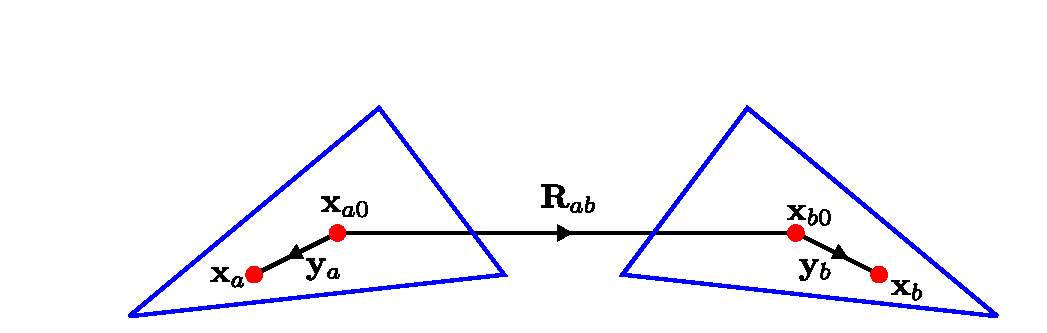
\includegraphics{figures/PPIDerivatives.pdf}
\caption{Notation for equation \ref{Rab}.}
\label{RabFigure}
\end{center}
\end{figure}
%####################################################################%
(In equation (\ref{ThreeHFunctions}), note that $h_\times$, 
unlike $h_\bullet$ and $h_\nabla$, depends on $\vb R$ in 
addition to $\vb y_a, \vb y_b$.)

Now we can take derivatives with respect to the components 
of $\vb R$. Putting $\vb r = \vb R + \vb y_a - \vb y_b)$, we have
\begin{align*}
  \pard{H_\bullet}{\vb R_i}
&= \int d\vb y_a \, \int d\vb y_b \,
   \vb r_i 
   h_\bullet(\vb y_a, \vb y_b)
   \psi\big(k, \vb R + \vb y_a - \vb y_b \big) 
\\
  \pard{H_\nabla}{\vb R_i}
&= \int d\vb y_a \, \int d\vb y_b \,
   \vb r_i 
   h_\nabla(\vb y_a, \vb y_b)
   \psi\big(k, \vb R + \vb y_a - \vb y_b \big)
\\
  \pard{H_\times}{\vb R_i}
&= 
   \int d\vb y_a \, \int d\vb y_b \,
   \vb r_i
   h_\times(\vb y_a, \vb y_b, \vb R)
   \zeta\big(k, \vb R + \vb y_a - \vb y_b \big)
\\
&\qquad + 
   \int d\vb y_a \, \int d\vb y_b \,
   \pard{h_\times(\vb y_a, \vb y_b, \vb R)}{\vb R_i}
   \psi\big(k, \vb R + \vb y_a - \vb y_b \big)
\end{align*}
In the last line, we put
$$ \zeta(k, r) = \Big[ (ikr)^2 -3ikr + 3\Big]\frac{e^{ikr}}{4\pi r^5}$$
[which is defined such that $\nabla \psi(k,|\vb r|) = \vb r \zeta(k, |\vb r|)$]
and we have 
\begin{align*}
 \pard{ h_\times(\vb y_a, \vb y_b, \vb R)}{\vb R_i}
&=\pard{}{\vb R_i} 
   \bigg\{ \Big[ (\vb y_a - \vb Q_a) \times (\vb y_b - \vb Q_b) \Big]
           \cdot \vb R 
   \bigg\}
\\
&= \Big[ (\vb y_a - \vb Q_a) \times (\vb y_b - \vb Q_b) \Big]_i.
\end{align*}

\subsubsection*{Desingularization}

%====================================================================%
\begin{align*}
  \pard{H_\bullet}{\vb R_i}
&= \iint \vb r_i \vb h_\bullet \psi
\\
&= \iint \vb r_i h_{\bullet} \psi\supt{DS}
   +\sum_{n=0}^4 \frac{(ik)^n}{4\pi} B_n 
    \iint \vb r_i h_{\bullet} r^{n-3}
\\[10pt]
%--------------------------------------------------------------------%
  \pard{H_\nabla}{\vb R_i}
&= \iint \vb r_i h_\nabla \psi  
\\
&= \left[ \iint \vb r_i h_{\nabla} \psi\supt{DS}
                 +\sum_{n=0}^4 \frac{(ik)^n}{4\pi} B_n 
                  \iint \vb r_i h_{\nabla } r^{n-3}
           \right]
\\[10pt]
%--------------------------------------------------------------------%
  \pard{H_\times}{\vb R_i}
&=   \iint \vb r_i h_\times \zeta
   + \iint \left( \pard{h_\times}{\vb R_i}\right) \psi
\\
%--------------------------------------------------------------------%
&= \iint \vb r_i h_{\times} \zeta\supt{DS}
    +\iint \left(\pard{h_\times}{\vb R_i}\right)\psi\supt{DS}   
\\ 
&\qquad
   +\left[ \sum_{n=0}^5 \frac{(ik)^n}{4\pi} C_n 
                   \iint \vb r_i h_{\times } r^{n-5}
            \right]
   + \left[ \sum_{n=0}^4 \frac{(ik)^n}{4\pi} B_n 
            \iint \left( \pard{h_{\times}}{\vb R_i}\right) r^{n-3}
     \right]
\end{align*}
%====================================================================%
In the last line here we used
$$ \zeta\supt{DS}(k, r) = 
   \Big[ (ikr)^2 -3ikr + 3\Big]\frac{\texttt{ExpRel(ikr,4)}}{4\pi r^5} 
$$
and the $C_n$ coefficients are 
$$ C_0=3, \qquad C_1=0, \qquad C_2=-\frac{1}{2}, 
   \qquad C_3=C_4=0, \qquad C_5=\frac{1}{6}.
$$

%%%%%%%%%%%%%%%%%%%%%%%%%%%%%%%%%%%%%%%%%%%%%%%%%%%%%%%%%%%%%%%%%%%%%%
%%%%%%%%%%%%%%%%%%%%%%%%%%%%%%%%%%%%%%%%%%%%%%%%%%%%%%%%%%%%%%%%%%%%%%
%%%%%%%%%%%%%%%%%%%%%%%%%%%%%%%%%%%%%%%%%%%%%%%%%%%%%%%%%%%%%%%%%%%%%%
\newpage

%%%%%%%%%%%%%%%%%%%%%%%%%%%%%%%%%%%%%%%%%%%%%%%%%%%%%%%%%%%%%%%%%%%%%%
%%%%%%%%%%%%%%%%%%%%%%%%%%%%%%%%%%%%%%%%%%%%%%%%%%%%%%%%%%%%%%%%%%%%%%
%%%%%%%%%%%%%%%%%%%%%%%%%%%%%%%%%%%%%%%%%%%%%%%%%%%%%%%%%%%%%%%%%%%%%%
\newpage
\section{Other Panel Integrals}
\begin{figure}
\resizebox{\textwidth}{!}{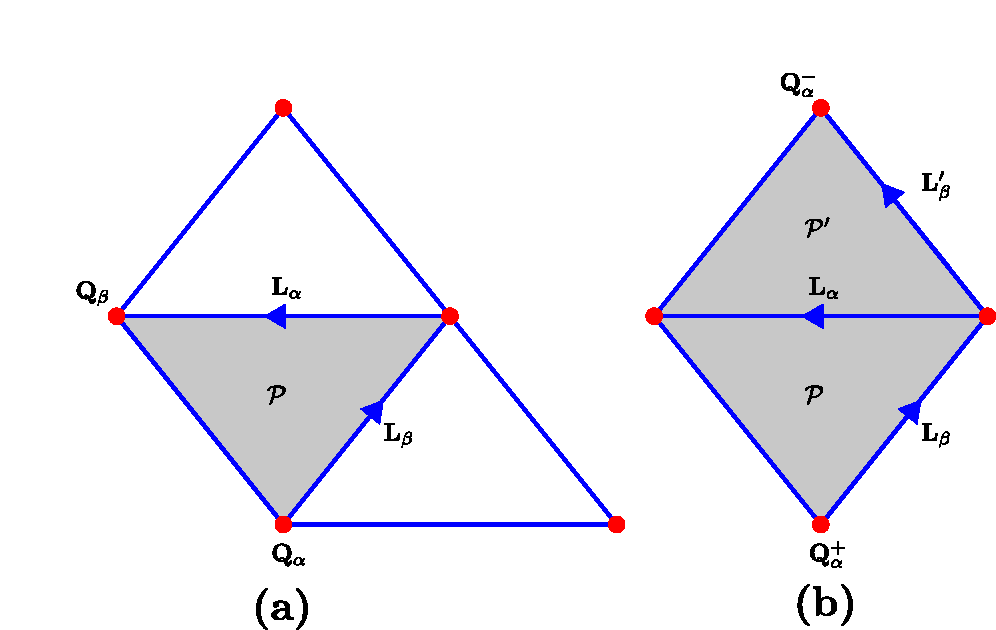
\includegraphics{OverlapIntegrals.pdf}}
\caption{Notation for computation of overlap integrals.}
\label{OverlapIntegralFigure}
\end{figure}

\subsection{Overlap Integral}

The overlap integral between two RWG basis functions is 
$$ O_{\alpha\beta}=
\Big<\vb f_\alpha \Big | \vb f_\beta\Big > 
=\int_{\text{\scriptsize sup }\vb f_\alpha\, \cap \,
        \text{\scriptsize sup }\vb f_\beta } 
  \vb f_\alpha(\vb x) \cdot \ \vb f_\beta(\vb x)
   \,d\vb x.
$$
If we think of $O_{\alpha\beta}$ as the $\alpha,\beta$ element of 
a matrix $\vb O$, then $\vb O$ is a very sparse matrix, with
at most 5 nonzero entries per row. Fix an interior edge 
$\vb L_\alpha$ in a triangular surface mesh and consider the 
basis function $\vb f_\alpha$ associated with this edge.
The only basis functions to have nonvanishing overlap with 
$\vb f_\alpha$ are \textbf{(1)} $\vb f_\alpha$ itself, and 
\textbf{(2)} basis functions associated with the four 
edges beside $\vb L_\alpha$ on the two panels that 
share $\vb L_\alpha$, such as $\vb L_\beta$ in Figure 
\ref{OverlapIntegralFigure}\textbf{(a)}.

\paragraph{The case $\alpha\ne \beta$.} 

Consider first the case of inequal basis functions
$\vb f_\alpha,\vb f_\beta$ that share a single
panel $\mathcal{P}$ [Figure \ref{OverlapIntegralFigure}\textbf{(a)}].
We parameterize points within $\mathcal{P}$ 
according to 
$$ \vb x=\vb Q_\alpha + u\vb L_\beta + v\vb L_\alpha, 
   \qquad 0\le u \le 1, \quad 0 \le v \le u.
$$
On $\mathcal{P}$, the two basis functions may be expressed in 
terms of this parameterization as 
\begin{align*} 
 \vb f_\alpha(\vb x) 
&= 
 \frac{\sigma^\alpha l_\alpha}{2A}
 \Big[u\vb L_\beta + v\vb L_\alpha\Big] 
\\
 \vb f_\beta(\vb x) 
&= \frac{\sigma^\beta l_\beta}{2A}
  \Big[ u\vb L_\beta + v\vb L_\alpha + (\vb Q_\alpha - \vb Q_\beta)\Big]
\\
&= \frac{\sigma^\beta l_\beta}{2A}
  \Big[ (u-1)\vb L_\beta + (v-1)\vb L_\alpha\Big]
\end{align*} 
Here $A$ is the area of $\mathcal{P}$ and $\sigma^\alpha = \pm 1$  
according as $\mathcal{P}$ is the positive or negative panel
associated with basis function $\vb f_\alpha$ (and similarly 
for $\sigma^{\beta}$), and we used the fact that 
$\vb Q_\alpha + \vb L_\beta + \vb L_\alpha = \vb Q_\beta.$

The overlap integral is 
\begin{align}
O_{\alpha\beta}
&=\int_{\mathcal{P}} \vb f_\alpha(\vb x) \cdot \vb f_\beta(\vb x)  \, d\vb x 
\nn
&=\frac{\sigma^\alpha \sigma^\beta l_\alpha l_\beta}{2A} 
  \int_0^1 \, du \, \int_0^u \, dv \, 
  \Big[ u \vb L_\beta + v\vb L_\alpha\Big]
 \cdot
  \Big[ (u-1) \vb L_\beta + (v-1)\vb L_\alpha\Big]
\nn
&=-\frac{\sigma^\alpha \sigma^\beta l_\alpha l_\beta}{24A} 
  \Big[ l_\alpha^2 + l_\beta^2 + 3\vb L_\alpha\cdot \vb L_\beta\Big]
\label{OAlphaBeta}
\end{align}

\paragraph{The case $\alpha=\beta$.}

In this case there are two panels that contribute
[Figure \ref{OverlapIntegralFigure}\textbf{(b)}].
The contribution of $\mathcal{P}$ is
\begin{align*}
\int_{\mathcal{P}} \vb f_\alpha(\vb x) \cdot \vb f_\alpha(\vb x)  \, d\vb x 
&=\frac{l_\alpha^2}{2A} 
  \int_0^1 \, du \, \int_0^u \, dv \, 
  \Big[ u \vb L_\beta + v\vb L_\alpha\Big]
 \cdot
  \Big[ u \vb L_\beta + v\vb L_\alpha\Big]
\\
&=\frac{l^2_\alpha}{24A} 
  \Big[ 3l_\alpha^2 + l_\beta^2 + 3\vb L_\alpha\cdot \vb L_\beta\Big].
\end{align*}
Adding the contribution of $\mathcal{P}^\prime$, 
the total overlap integral is 
\numeq{OAlphaAlpha}
{
O_{\alpha\alpha}
=\frac{l^2_\alpha}{24}
 \bigg\{ 
   \frac{1}{A}        \Big[ l_\alpha^2 + 3l_\beta^2 + 3\vb L_\alpha\cdot \vb L_\beta\Big]
 + \frac{1}{A^\prime} \Big[ l_\alpha^2 + 3l_\beta^{\prime 2} 
                            + 3\vb L_\alpha\cdot \vb L_\beta^\prime\Big]
 \bigg\}.
}

\subsection{Crossed Overlap Integral}

The crossed overlap integral between two RWG basis functions is 
$$ O^{\times}_{\alpha\beta}=
\Big<\vb f_\alpha \Big | \vbhat{n}\times \vb f_\beta\Big > 
=\int_{\text{\scriptsize sup }\vb f_\alpha\, \cap \,
        \text{\scriptsize sup }\vb f_\beta } 
  \vb f_\alpha(\vb x) \cdot \Big[\vbhat{n}(\vb x)\times  \vb f_\beta(\vb x)\Big]
   \,d\vb x
$$
where $\vbhat{n}(\vb x)$ is the surface normal at $\vb x$. 
(The direction of $\vbhat{n}$ must be chosen consistently; 
in {\sc libscuff} this is done by placing one or more 
\textit{reference points} inside closed objects and choosing 
the surface normal to each panel to point \textit{away}
from the nearest reference point.)

$ O^{\times}_{\alpha\beta}$ is only nonzero in 
the case of Figure \ref{OverlapIntegralFigure}\textbf{(b)}.
(In particular, the diagonal element 
$ O^{\times}_{\alpha\alpha}$ vanishes.)
Proceeding in analogy to the computation leading to 
equation (\ref{OAlphaBeta}), we find
\begin{align}
O^{\times}_{\alpha\beta}
&=\int_{\mathcal{P}} \vb f_\alpha(\vb x) \cdot 
                     \Big[\vbhat{n} \times \vb f_\beta(\vb x)\Big]  \, d\vb x 
\nn
&=\frac{\sigma^\alpha \sigma^\beta l_\alpha l_\beta}{2A} 
  \int_0^1 \, du \, \int_0^u \, dv \, 
  \Big[ u \vb L_\beta + v\vb L_\alpha\Big]
 \cdot
  \Big[ (u-1) \big(\vbhat{n}\times \vb L_\beta\big) + 
        (v-1) \big(\vbhat{n}\times \vb L_\alpha\big)
  \Big]
\nn
&=\frac{\sigma^\alpha \sigma^\beta l_\alpha l_\beta}{12A} 
  \Big[ \vb L_\alpha \cdot (\vbhat{n}\times \vb L_\beta) \Big]
\nn
&=\frac{\sigma^\alpha \sigma^\beta l_\alpha l_\beta}{12A} 
  \Big[ \vbhat{n} \cdot \big(\vb L_\beta\times \vb L_\alpha\big) \Big]
\nonumber
\intertext{by cyclic permutation of the triple vector product. But
the magnitude of the cross product here is just $\vbhat{n}$ times 
twice the panel area,}
&=\frac{\sigma^\alpha \sigma^\beta l_\alpha l_\beta}{12A} 
  \Big[ \vbhat{n} \cdot \big(\pm 2A\,\vbhat{n}\big) \Big]
\nn
&=\pm\frac{\sigma^\alpha \sigma^\beta l_\alpha l_\beta}{6}.
\label{OTimesAlphaBeta}
\end{align}
The $\pm$ sign is determined as follows: Suppose we start 
at vertex $\vb Q_\alpha$ and traverse the vertices of 
$\mathcal{P}$ by following $\vb L_\beta$, then $\vb L_\alpha$.
If in so doing we encounter the vertices of $\pan$ in 
the order $(0,1,2)$ or a cyclic permutation thereof, then
the $+$ sign holds in (\ref{OTimesAlphaBeta}); otherwise
(i.e. if we encounter the vertices in the order $(0,2,1)$ or 
a cyclic permutation thereof) the $-$ sign holds.

An easy way to determine this sign is to look at the 
indices within $\mathcal{P}$ of vertices $\vb Q_\beta$
and $\vb Q_\alpha$. Call these $I_\pan(\vb Q_\beta)$ and 
$I_\pan(\vb Q_\alpha)$, respectively; they are integers
defined modulo 3. Then the sign in (\ref{OTimesAlphaBeta})
is 
$$ \text{sign in equation (\ref{OTimesAlphaBeta})} 
   = 
   \begin{cases}
   +, \quad &\text{if } I_\pan(\vb Q_\beta)
                       -I_\pan(\vb Q_\alpha)
                        \equiv 2 \text{ mod } 3 
   \\
   -, \quad &\text{if } I_\pan(\vb Q_\beta)
                       -I_\pan(\vb Q_\alpha)
                        \equiv 1 \text{ mod } 3.
   \end{cases}
$$

%%%%%%%%%%%%%%%%%%%%%%%%%%%%%%%%%%%%%%%%%%%%%%%%%%%%%%%%%%%%%%%%%%%%%%
%%%%%%%%%%%%%%%%%%%%%%%%%%%%%%%%%%%%%%%%%%%%%%%%%%%%%%%%%%%%%%%%%%%%%%
%%%%%%%%%%%%%%%%%%%%%%%%%%%%%%%%%%%%%%%%%%%%%%%%%%%%%%%%%%%%%%%%%%%%%%
\newpage

\include{lsInnardsSections/CartesianMultipoleMoments}
%%%%%%%%%%%%%%%%%%%%%%%%%%%%%%%%%%%%%%%%%%%%%%%%%%%%%%%%%%%%%%%%%%%%%%
%%%%%%%%%%%%%%%%%%%%%%%%%%%%%%%%%%%%%%%%%%%%%%%%%%%%%%%%%%%%%%%%%%%%%%
%%%%%%%%%%%%%%%%%%%%%%%%%%%%%%%%%%%%%%%%%%%%%%%%%%%%%%%%%%%%%%%%%%%%%%
\newpage
\section{Spherical Multipole Moments}

\subsection*{Definition of the Spherical Multipole Moments}

Following Jackson and other authors, I define the 
electric and magnetic spherical multipole moments of a localized source 
distribution to be the coefficients in a spherical-wave
expansion of the fields away from the source regions:
\begin{subequations}
\begin{align}
 \vb E(\vb r) &= \sum_{\ell m} \Big\{  a\supt{M}_{\ell,m} \MMExt_{\ell m}(\vb r)
                                      +a\supt{E}_{\ell,m} \NNExt_{\ell m}(\vb r)
                               \Big\}
\\
 \vb H(\vb r) &= \frac{1}{Z}
                 \sum_{\ell m} \Big\{ -a\supt{M}_{\ell,m} \NNExt_{\ell m}(\vb r)
                                      +a\supt{N}_{\ell,m} \MMExt_{\ell m}(\vb r)
                               \Big\}
\end{align}
\label{SphericalMultipoleDefinitions}
\end{subequations}
where $Z$ is the wave impedance of the medium ($Z=377\,\Omega$ for vacuum).
Note that my $a\supt{M}_{\ell,m}, a\supt{E}_{\ell,m}$ coefficients
are not normalized in quite the same way as Jackson's
$a\subt{$M$}(l,m), a\subt{$E$}(l,m)$ coefficients; 
the relationship is 
$$ a\supt{M}_{\ell,m} = Z_0 a\subt{$M$}(l,m), \qquad 
   a\supt{E}_{\ell,m} = Z_0 \frac{i}{k} a\subt{$E$}(l,m)
$$
Jackson gives expressions (equations 9.167-8) for computing 
the $a$ coefficients for given source distributions; however, 
these expressions are not convenient for our 
purposes.\footnote{In particular, applying Jackson's expressions
directly would require evaluating integrals over the quantity 
$\nabla\cdot \big[\vb r \times \vb f\supt{RWG}(\vb r)\big]$,
which vanishes in the \textit{interior} of an RWG panel but makes
nonzero contributions at the \textit{edges}. This complication
makes Jackson's expressions somewhat unwieldy in our case, 
whereas the approach outlined above is computationally 
straightforward.} Instead, in the following sections I outline
an alternative approach for recovering the $a$ coefficients
from known source distributions.

\subsection*{Expansion of the Dyadic Green's Functions in Spherical Helmholtz Solutions}

This approach is based on the well-known spherical-wave expansion 
of the dyadic Green's functions of Section \ref{DyadicGreensFunctionsSection}.
[In the following expression, the $\rho$ and $\sigma$ subscripts run over
spherical vector components ($r,\theta,\phi$.)]

\begin{subequations}
\begin{align}
  G_{\rho\sigma} (k; \vb r-\vb r^\prime)
&=\hspace{0.09in} ik
  \sum_{\ell m} 
  \Big\{ 
     \MMExt_{\ell m \rho}( k, \vb r_>)
     \MMInt^*_{\ell m \sigma}( k, \vb r_<) 
   + \NNExt_{\ell m \rho}( k, \vb r_>)
     \NNInt^*_{\ell m \sigma}( k, \vb r_>) 
  \Big\}
\\
  C_{\rho\sigma} (k; \vb r-\vb r^\prime)
&=ik
  \sum_{\ell m} 
  \Big\{ 
     \NNExt_{\ell m \rho}( k, \vb r_>)
     \MMInt^*_{\ell m \sigma}( k, \vb r_<) 
   - \MMExt_{\ell m \rho}( k, \vb r_>)
     \NNInt^*_{\ell m \sigma}( k, \vb r_>) 
  \Big\}
\end{align}
\label{GCExpansions}
\end{subequations}
(Note: The expansion for $\vb C$ here assumes that 
$|\vb r|>|\vb r^\prime|.$ In the opposite case in 
which 
$|\vb r|<|\vb r^\prime|,$ the above expression for $\vb C$
acquires a minus sign.)

\subsection*{Fields due to localized current distributions}

Now consider the fields arising from localized surface electric
and magnetic current distributions $\vb K(\vb x)$ and $\vb N(\vb x):$
\begin{align*}
 \vb E(\vb r) 
&= 
   ik\int \Big\{ Z\vb G(k, \vb r-\vb r^\prime) \cdot \vb K(\vb r^\prime)
                 +\vb C(k, \vb r-\vb r^\prime) \cdot \vb N(\vb r^\prime)
          \Big\} \, d\vb r^\prime
\\
 \vb H(\vb r) 
&= 
   ik\int \Big\{ -\vb C(k, \vb r-\vb r^\prime) \cdot \vb K(\vb r^\prime)
                 +\frac{1}{Z}\vb G(k, \vb r-\vb r^\prime) \cdot \vb N(\vb r^\prime)
          \Big\}\,d\vb r^\prime.
\end{align*}
Insert the expansions (\ref{GCExpansions}) and assume that the 
field evaluation point will always be further from the origin than
the source current point: 
\begin{subequations}
\begin{align*}
 \vb E(\vb r) 
&= 
 -k^2 \sum_{\ell m} 
       \Bigg\{ \BMMExt_{\ell m}(\vb r) \cdot 
               \bigg[   \INP{ \BMMInt_{\ell m} }{Z \vb K}
                      - \INP{ \BNNInt_{\ell m} }{\vb N}
               \bigg]
\\
&\hspace{1.0in}
             + \BNNExt_{\ell m}(\vb r) \cdot 
               \bigg[   \INP{ \BNNInt_{\ell m} }{Z \vb K}
                      + \INP{ \BMMInt_{\ell m} }{\vb N}
               \bigg]
       \Bigg\}
\\[8pt]
 \vb H(\vb r) 
&= -\frac{k^2}{Z_0} \sum_{\ell m} 
       \Bigg\{ \BMMExt_{\ell m}(\vb r) \cdot 
               \bigg[   \INP{ \BNNInt_{\ell m} }{Z\vb K}
                      + \INP{ \BMMInt_{\ell m} }{\vb N}
               \bigg]
\\
&\hspace{1.0in}
             + \BNNExt_{\ell m}(\vb r) \cdot 
               \bigg[ - \INP{ \BMMInt_{\ell m} }{Z\vb K}
                      + \INP{ \BNNInt_{\ell m} }{\vb N}
               \bigg]
       \Bigg\}
\end{align*}
\label{SphericalFieldExpansions}
\end{subequations}

Comparing (\ref{SphericalFieldExpansions}) with the definitions
(\ref{SphericalMultipoleDefinitions}) now allows us to read off
the expressions for $a\sups{E,M}$ in terms of the source
distributions $\vb K$ and $\vb N$: 

%====================================================================%
%====================================================================%
%====================================================================%
\begin{subequations}
\begin{align}
a\sups{M}_{\ell,m}
 &= -k^2\bigg[ \INP{ \BMMInt_{\ell m} }{Z\vb K}
              -\INP{ \BNNInt_{\ell m} }{\vb N}
        \bigg]
\\
a\sups{E}_{\ell,m}
 &= -k^2\bigg[  \INP{ \BNNInt_{\ell m} }{Z\vb K}
               +\INP{ \BMMInt_{\ell m} }{\vb N}
        \bigg]
\end{align}
\label{SphericalMultipolesFromKN}
\end{subequations}
%====================================================================%
%====================================================================%
%====================================================================%

%%%%%%%%%%%%%%%%%%%%%%%%%%%%%%%%%%%%%%%%%%%%%%%%%%%%%%%%%%%%%%%%%%%%%%
%%%%%%%%%%%%%%%%%%%%%%%%%%%%%%%%%%%%%%%%%%%%%%%%%%%%%%%%%%%%%%%%%%%%%%
%%%%%%%%%%%%%%%%%%%%%%%%%%%%%%%%%%%%%%%%%%%%%%%%%%%%%%%%%%%%%%%%%%%%%%
\newpage

%%%%%%%%%%%%%%%%%%%%%%%%%%%%%%%%%%%%%%%%%%%%%%%%%%%%%%%%%%%%%%%%%%%%%%
%%%%%%%%%%%%%%%%%%%%%%%%%%%%%%%%%%%%%%%%%%%%%%%%%%%%%%%%%%%%%%%%%%%%%%
%%%%%%%%%%%%%%%%%%%%%%%%%%%%%%%%%%%%%%%%%%%%%%%%%%%%%%%%%%%%%%%%%%%%%%
\newpage
\section{Evaluation of the fields at panel centroids}

It is useful to have expressions for the $\vb E$ and $\vb H$
fields at the centroids of the triangular panels in the
discretization of object surfaces. Of course, the solution 
of the EFIE or PMCHW equations automatically gives us the 
\textit{tangential} components of the fields on the object
surfaces, but to get the normal components we must do a little
more work. 

Thus, consider the fields at a point lying a distance $z$
above the centroid of a panel in the direction of the 
outward-pointing panel normal. Let $\vbrho=(x,y)$ be the
in-plane coordinate vector. The normal $\vb E-$field is given by
%====================================================================%
\begin{align}
E_z(z) 
 &= \int d\vbrho \, \Big\{ 
             \Gamma_{zx}\supt{EE}(\vbrho, z) K_x(\vbrho) 
            +\Gamma_{zy}\supt{EE}(\vbrho, z) K_y(\vbrho) 
           \Big\}
\nonumber \\
&\qquad
   + \int d\vbrho \, \Big\{ 
             \Gamma_{zx}\supt{EM}(\vbrho, z) N_x(\vbrho) 
            +\Gamma_{zy}\supt{EM}(\vbrho, z) N_y(\vbrho) 
           \Big\}.
\label{Ezz}
\end{align}
%====================================================================%
Anticipating that the final answers will involve the 
first derivatives of $\vb K$ and $\vb N$ at the origin (i.e. the panel 
centroid), I write
%====================================================================%
\begin{align*}
 K_x(\vbrho) &= K_x^{(00)} + x K_x^{(10)} + y K_x^{(01)} + xyK_x^{(11)}
  + \cdots 
\\
 K_y(\vbrho) &= K_y^{(00)} + x K_y^{(10)} + y K_y^{(01)} + xyK_y^{(11)}
  + \cdots
\end{align*}
(where $K^{(pq)}$ is short 
for $|\partial^{p+q} K/\partial^p x \partial^q y|_{\vbrho=0}$)
and similarly for the components of $\vb N$.
%====================================================================%
Also, the components of the $\Gamma$ tensors that I will need are
%====================================================================%
\begin{align*}
 \Gamma\supt{EE}_{zx} &= i k Z zx \big[-3 + 3ikr - (ikr)^2\big]
  \frac{e^{ikr}}{4\pi (ik)^2 r^5}
\\
 \Gamma\supt{EE}_{zy} &= i k Z zy \big[-3 + 3ikr - (ikr)^2\big]
  \frac{e^{ikr}}{4\pi (ik)^2 r^5}
\\
 \Gamma\supt{EM}_{zx} &= i k y \big[-1 + ikr\big]
  \frac{e^{ikr}}{4\pi (ik) r^3}
\\
 \Gamma\supt{EM}_{zy} &= -i k x \big[-1 +ikr\big]
  \frac{e^{ikr}}{4\pi (ik) r^3}
\end{align*}
%====================================================================%
where $r=\sqrt{\vbrho^2 + z^2}$ and $k,Z$ are the wavenumber and
wave impedance for the medium in question.
Now I insert everything into (\ref{Ezz}) and note that terms linear
in $x$ and/or $y$ vanish under the angular portion of the $d\vbrho$
integration:
$$ \int d\vbrho 
   \left\{ \begin{array}{c} 1 \\ x \\ y \\ x^2 \\xy \\y^2 \end{array}
   \right\}
   =2\pi \int \, \rho d\rho 
   \left\{ \begin{array}{c} 1 \\ 0 \\ 0 \\ \rho^2/2 \\ 0 \\ \rho^2/2 \end{array}
   \right\}
$$
%====================================================================%
This yields
\begin{align*}
 E_z(z) 
&= \frac{Z \big( K_x^{(10)} + K_y^{(01)} \big)}{4ik}  
   \cdot z \cdot \int_0^\infty \, \rho^3 d\rho \, \big[-3 + 3ikr - (ikr)^2\big] 
   \frac{e^{ikr}}{r^5}
\\
&\qquad
 + \frac{\big( N_x^{(01)} - N_y^{(10)} \big)}{4}  
   \int_0^\infty \, \rho^3 d\rho \, \big[-1 + ikr ] 
   \frac{e^{ikr}}{r^3}.
\end{align*}
%====================================================================%
The prefactor in the second term here involves the $z$ component of the 
curl of the magnetic current, $\nabla \times \vb N$; but the curl of an 
RWG basis function vanishes in the interior of the panels on which the 
function is defined, so this term does not contribute.

On the other hand, the first term here is proportional to $\nabla \cdot \vb K$.
Change integration variables to 
$r=\sqrt{\rho^2 + z^2}, \,\, r\,dr = \rho\, d\rho:$
%====================================================================%
\begin{align*}
 E_z(z) 
&= \frac{Z \big (\nabla \cdot \vb K \big)}{4ik} 
   \cdot z \cdot \int_z^\infty \, dr (r^2 - z^2) \, \big[-3 + 3ikr - (ikr)^2\big] 
   \frac{e^{ikr}}{r^4}
\end{align*}
The only terms in the integrand that lead to nonvanishing results in the 
$z\to 0$ limit are those coming from the $-3$ term in the square brackets:
%====================================================================%
\begin{align*}
 -3z\cdot \int_z^\infty \left[ \frac{1}{r^2} - \frac{z^2}{r^4} \right]dr 
&=
  3z\cdot\left| \frac{1}{r} - \frac{z^2}{3r^3} \right|_{z}^\infty
\\
&=2
\end{align*}
%====================================================================%
and thus 
\numeq{Ezz2}
{
   \lim_{z\to 0}E_z(z) 
   = \frac{Z(\nabla \cdot \vb K)}{2ik} 
   = \frac{(\nabla \cdot \vb K)}{2i\epsilon \omega } 
   = \frac{\sigma}{2\epsilon}
}
where $\sigma=\frac{1}{i\omega}\nabla \cdot \vb K$ is 
the surface charge density at the panel centroid. 

Equation (\ref{Ezz2}) is of course just the result we 
would have predicted on the basis of electrostatic 
arguments, but it is useful to see here how it follows 
from our full frequency-dependent formalism.

Meanwhile, an analogous calculation for the magnetic field yields
\numeq{Hzz}
{\lim_{z\to 0}H_z(z) 
   = -\frac{(\nabla \cdot \vb N)}{2i\mu\omega}.
   = -\frac{(\nabla \cdot \vb N)}{2ik Z}.
}
Note the minus sign compared to (\ref{Ezz2}).

%%%%%%%%%%%%%%%%%%%%%%%%%%%%%%%%%%%%%%%%%%%%%%%%%%%%%%%%%%%%%%%%%%%%%%
%%%%%%%%%%%%%%%%%%%%%%%%%%%%%%%%%%%%%%%%%%%%%%%%%%%%%%%%%%%%%%%%%%%%%%
%%%%%%%%%%%%%%%%%%%%%%%%%%%%%%%%%%%%%%%%%%%%%%%%%%%%%%%%%%%%%%%%%%%%%%
\newpage

\newcommand{\GammaBar}{\overline{\BG}}
\newcommand{\GBar}{\overline{G}}
\newcommand{\CBar}{\overline{C}}
\newcommand{\VBGBar}{\overline{\vb G}}
\newcommand{\VBCBar}{\overline{\vb C}}
\newcommand{\KB}{\vb k\subt{B}}

%%%%%%%%%%%%%%%%%%%%%%%%%%%%%%%%%%%%%%%%%%%%%%%%%%%%%%%%%%%%%%%%%%%%%
%%%%%%%%%%%%%%%%%%%%%%%%%%%%%%%%%%%%%%%%%%%%%%%%%%%%%%%%%%%%%%%%%%%%%
%%%%%%%%%%%%%%%%%%%%%%%%%%%%%%%%%%%%%%%%%%%%%%%%%%%%%%%%%%%%%%%%%%%%%
\section{BEM formulations for PBC bodies}

%=================================================
%=================================================
%=================================================
\subsection{Scattered field of an infinite PEC surface}

Consider the scattered field produced by an 
induced surface-current density $\vb K(\vb x)$ on
an infinite PEC surface $\mc S_\infty$:
%====================================================================%
\begin{align}
  \vb E\sups{scat}(\vb x)
&=
  \int_{\mc S_\infty} 
   \BG\supt{EE}(\vb x, \vb x^\prime)
   \cdot 
   \vb K(\vb x^\prime)d\vb x^\prime
\\
&=
  ikZ_0
  \int_{\mc S_\infty} 
   \vb G(\vb x, \vb x^\prime) 
   \cdot 
   \vb K(\vb x^\prime)d\vb x^\prime
\label{EScatPBC}
\end{align}
where $k=\omega/c$ ($\omega$ is the angular frequency
at which we are working) and $Z_0$ is the impedance
of free space (assume we are in vacuum for now).
If we now suppose that 
%====================================================================%
\begin{itemize}
 \item the surface $\mc S_\infty$ consists of an infinite lattice
       of copies of a unit-cell surface $\mc S_0$ translated through
       two-dimensional lattice vectors of the form 
       \numeq{LatticeVectors}{\vb L=n_1 \vb L_1 + n_2\vb L_2}
       and
 \item the surface current respects this periodicity in the 
       Bloch sense, i.e. we have
       \numeq{KPeriodicity}
       {\vb K(\vb x+\vb L)
          = e^{i\KB \cdot \vb L} \, \vb K(\vb x)
       }
       for some Bloch vector $\KB$
\end{itemize}
%====================================================================%
then I can write the scattered field (\ref{EScatPBC}) as an integral
over just the unit cell:
%====================================================================%
\begin{align}
   \vb E\sups{scat}(\vb x)
&= ikZ_0 
   \sum_{\vb L}
   \int_{\mc S_0}
   \vb G(\vb x, \vb x^\prime+\vb L)
   \cdot 
   \vb K(\vb x^\prime + \vb L ) \, d\vb x^\prime
\nn
&= ikZ_0
   \int_{\mc S_0}
   \underbrace{
   \left\{
   \sum_{\vb L}
   e^{i\KB \cdot \vb L}
   \vb G(\vb x, \vb x^\prime+\vb L)
   \right\}
              }_{\VBGBar(\vb x, \vb x^\prime)}
   \cdot 
   \vb K(\vb x^\prime) \, d\vb x^\prime
\nn
&= ikZ_0 
   \int_{\mc S_0}
   \VBGBar(\vb x, \vb x^\prime)
   \cdot 
   \vb K(\vb x^\prime) \, d\vb x^\prime
\label{EScatPBC}
\end{align}
where $\VBGBar$ is the dyadic periodic Green's function,
whose properties we now discuss.

%%%%%%%%%%%%%%%%%%%%%%%%%%%%%%%%%%%%%%%%%%%%%%%%%%%%%%%%%%%%%%%%%%%%%%
%%%%%%%%%%%%%%%%%%%%%%%%%%%%%%%%%%%%%%%%%%%%%%%%%%%%%%%%%%%%%%%%%%%%%%
%%%%%%%%%%%%%%%%%%%%%%%%%%%%%%%%%%%%%%%%%%%%%%%%%%%%%%%%%%%%%%%%%%%%%%
\subsection{Periodic Green's functions}

The dyadic periodic Green's function introduced in 
(\ref{EScatPBC}) is 
%====================================================================%
\begin{align*}
 \VBGBar(\vb x, \vb x^\prime)
&=\sum_{\vb L} e^{i\KB \cdot \vb L}\vb G(\vb x, \vb x^\prime+\vb L)
\\
 \VBGBar(\vb x, \vb x^\prime)
&=\sum_{\vb L} e^{i\KB \cdot \vb L}\vb G(\vb x-\vb x^\prime-\vb L)
\intertext{with cartesian components}
 \GBar_{ij}(\vb x, \vb x^\prime)
&=\sum_{\vb L} e^{i\KB \cdot \vb L}G_{ij}(\vb x-\vb x^\prime-\vb L)
\\
&=\sum_{\vb L} 
   e^{i\KB \cdot \vb L} 
  \left[
   \Big( \delta_{ij} + \frac{1}{k^2}\partial_i \partial_j\Big)
   \frac{e^{ik|\vb x - \vb x^\prime - \vb L|}}
        {4\pi|\vb x - \vb x^\prime - \vb L|}
  \right]
\intertext{Interchange differentiation and summation:}
&=
  \Big( \delta_{ij} + \frac{1}{k^2}\partial_i \partial_j\Big)
  \underbrace{
  \left\{ \sum_{\vb L} 
          e^{i\KB \cdot \vb L}
          \frac{e^{ik|\vb x - \vb x^\prime - \vb L|}} 
          {4\pi|\vb x - \vb x^\prime - \vb L |}
   \right\}}_{\GBar_0(\vb x-\vb x^\prime)}
\end{align*}
where $\GBar_0$ is the scalar periodic Green's function.
(\lss computes $\GBar_0$ and its derivatives using Ewald
summation together with an interpolation-table method
discussed below.)
%====================================================================%

I will also need the periodic version of the $\vb C$ dyadic
(or ``MFIE kernel''),
%====================================================================%
\begin{align*}
  \VBCBar(\vb x, \vb x^\prime)
 &=\sum_{\vb L} e^{i\KB \cdot \vb L}\vb C(\vb x-\vb x^\prime-\vb L)
\intertext{with components}
  \CBar_{ij}(\vb x, \vb x^\prime)
 &=\sum_{\vb L} e^{i\KB \cdot \vb L}C_{ij}(\vb x-\vb x^\prime-\vb L)
\\
 &=\frac{1}{ik}\epsilon_{ij\ell} \partial_\ell 
   \sum_{\vb L} e^{i\KB \cdot \vb L}G_0(\vb x-\vb x^\prime-\vb L).
\end{align*}
%====================================================================%

\paragraph{Transpositional symmetries of periodic Green's functions}

The non-periodic $\vb G$ and $\vb C$ dyadics are invariant 
under simultaneous transposition of indices and inversion of 
argument:
%--------------------------------------------------------------------%
\numeq{GCTranspose}
{
  G_{ij}(\vb r) = G_{ji}(-\vb r), \qquad 
  C_{ij}(\vb r) = C_{ji}(-\vb r).
}
%--------------------------------------------------------------------%
Now consider the implications of this for the periodic dyadics. In
particular, we write
%--------------------------------------------------------------------%
\begin{subequations}
\begin{align}
  \GBar_{ij}(\KB; \vb x, \vb x^\prime)
 &=\sum_{\vb L} e^{i\KB \cdot \vb L}G_{ij}(\vb x-\vb x^\prime-\vb L)
\nonumber
\intertext{Use (\ref{GCTranspose}):}
 &=\sum_{\vb L} e^{i\KB \cdot \vb L}G_{ji}(\vb x^\prime-\vb x^\prime+\vb L)
\nonumber
\intertext{Relabel the summation variable according to $\vb L \to -\vb L$:}
 &=\sum_{\vb L} e^{-i\KB \cdot \vb L}G_{ji}(\vb x^\prime-\vb x-\vb L)
\nn
 &=\GBar_{ji}(-\KB; \vb x^\prime, \vb x)
\intertext{and similarly}
  \CBar_{ij}(\KB; \vb x, \vb x^\prime)
&=\CBar_{ji}(-\KB; \vb x^\prime, \vb x).
\end{align}
\label{TranspositionSymmetries}
\end{subequations}
%--------------------------------------------------------------------%
Thus the periodic $\vb G$ and $\vb C$ dyadics are invariant
under simultaneous transposition of indices, interchange of 
$\vb x,\vb x^\prime$, and inversion of the Bloch vector.

\paragraph{Translational symmetries of periodic Green's functions}

Suppose the lattice basis vectors are $\vb L_1, \vb L_2$.
Then we can write the sum that defines the scalar periodic Green's
function in the form
%====================================================================%
\begin{align*}
\GBar_0(\vb r)
&= \sum_{n_1, n_2=-\infty}^\infty 
   e^{i\KB \cdot(n_1 \vb L_1 + n_2 \vb L_2)}
     G_0(\vb r - n_1\vb L_1 - n_2 \vb L_2)
\end{align*}
%====================================================================%
Now consider evaluating $\GBar$ at an argument displaced
through one full lattice basis vector:
\begin{align*}
 \VBGBar(\vb r + \vb L_1) 
&= \sum_{n_1, n_2=-\infty}^\infty 
   e^{i\KB \cdot (n_1\vb L_1 + n_2\vb L_2)}
   G_0( \vb r + \vb L_1 - n_1 \vb L_1 - n_2 \vb L_2)
\intertext{Add and subtract $\vb L_1$ in the exponent of 
           the Bloch factor:}
&= e^{i\KB \cdot \vb L_1}
   \sum_{n_1, n_2=-\infty}^\infty 
   e^{i\KB \cdot [(n_1-1)\vb L_1 + n_2\vb L_2]}
   G_0( \vb r -(n_1-1)\vb L_1 - n_2 \vb L_2)
\intertext{Now just redefine $n_1\to n_1-1$ in the infinite sum:}
&= e^{i\KB \cdot \vb L_1} \VBGBar( \vb r ).
\end{align*}
%====================================================================%
More generally, for any lattice vector $\vb L$ I have
$$
 \VBGBar(\vb r + \vb L)
 = e^{i\KB \cdot \vb L}\VBGBar(\vb r).
$$

%=================================================
%=================================================
%=================================================
\subsection{Discretized EFIE formulation}

Now consider solving for $\vb K(\vb x)$ in the presence
of illumination by an external Bloch-periodic 
field $\vb E\sups{inc}$.
We suppose that the current distribution in the unit cell 
is represented approximately by an expansion in basis
functions $\{\vb b_\alpha(\vb x)\}:$
%====================================================================%
\numeq{KExpansionPBC}
{\vb K(\vb x) \approx k_\alpha \vb b_\alpha(\vb x).}
%====================================================================%
The electric-field integral equation reads
%====================================================================%
\numeq{EFIE}
{\vb E\sups{scat}_\parallel(\vb x)
   =-\vb E\sups{inc}_\parallel(\vb x).
}
%====================================================================%
As in the usual compact-surface case, inserting (\ref{EScatPBC}) 
and (\ref{KExpansionPBC}) and testing with each element in the set 
$\{\vb b_\alpha\}$ yields a discretized PBC EFIE:
%====================================================================%
\begin{align}
 \sum_{\beta}
 \underbrace{
   \Big \langle \vb b_\alpha \Big|
   ikZ_0\VBGBar    
   \Big| \vb b_\beta \Big\rangle
            }_{\vb M_{\alpha\beta}} 
   k_\beta
&=-\Big \langle \vb b_\alpha \Big | \vb E\sups{inc} \Big\rangle
\label{PBCEFIE}
\end{align}
%====================================================================%
In other words, we obtain a formulation that looks exactly
like the formulation for compact objects, with the only
difference being that the elements of the BEM matrix
involve the $\VBGBar$ kernel in place of the usual 
$\vb G$ dyadic Green's function.

Note that the testing procedure that leads to 
(\ref{PBCEFIE}) is only testing the satisfaction
of equation (\ref{EFIE}) for points $\vb x$
\textit{in the unit cell.} However, the Bloch-periodicity
of the incident and scattered fields ensures that
satisfaction of the equation throughout the unit cell
implies its satisfaction everywhere.

%=================================================
%=================================================
%=================================================
\subsection{Symmetries of the PBC BEM matrix}

For a PEC structure, the $\alpha,\beta$ element of 
the BEM matrix is 
%--------------------------------------------------------------------%
\begin{align*}
 M_{\alpha\beta}(\KB)
&= ik\Big \langle \vb b_\alpha \Big|
    \VBGBar(\KB)
   \Big| \vb b_\beta \Big\rangle
\\
&= ik\int 
   \Big\{ 
   b_{\alpha i}(\vb x_\alpha) 
   \underbrace{\GBar_{ij}(\KB; \vb x_\alpha , \vb x_\beta)}
             _{=\GBar_{ji}(-\KB; \vb x_\beta , \vb x_\alpha )}
   b_{\beta j}(\vb x_\beta) 
   \Big\}\, d\vb x_\alpha d\vb x_\beta
\\
&= ik\Big \langle \vb b_\beta\Big|
    \VBGBar(-\KB)
   \Big| \vb b_\alpha\Big\rangle
\\
&=M_{\beta\alpha}(-\KB)
\end{align*}
%--------------------------------------------------------------------%
where we used equation (\ref{TranspositionSymmetries}a). 
For a dielectric structure, the matrix elements also involve
inner products with $\VBCBar$ dyadics, but since $\VBCBar$ satisfies
the same symmetry as $\VBGBar$ (\ref{TranpositionSymmetry}b), 
a similar equation holds in that case.

Thus in general for both PEC and non-PEC BEM matrices we have
\numeq{PBCMatrixTranspose}
{\vb M(\KB) = \Big[ \vb M(-\KB) \Big]^T}
where $T$ denotes the \textit{non-conjugate} transpose.

\subsubsection*{Symmetries in the imaginary frequency case}

For equilibrium Casimir computations we need elements
of the BEM matrix at imaginary frequencies. 
%====================================================================%
$$ \vb M(i\xi, \KB) = \vb M(i\xi, \KB)^\dagger $$
%====================================================================%

%%%%%%%%%%%%%%%%%%%%%%%%%%%%%%%%%%%%%%%%%%%%%%%%%%%%%%%%%%%%%%%%%%%%%%
%%%%%%%%%%%%%%%%%%%%%%%%%%%%%%%%%%%%%%%%%%%%%%%%%%%%%%%%%%%%%%%%%%%%%%
%%%%%%%%%%%%%%%%%%%%%%%%%%%%%%%%%%%%%%%%%%%%%%%%%%%%%%%%%%%%%%%%%%%%%%
\section{PBC geometries in {\sc scuff-em}}

%=================================================
%=================================================
%=================================================
\subsection{Overview}

\lss supports Bloch-periodic boundary conditions for
periodically repeated geometries. In this case,

\begin{itemize}
 \item The \texttt{.scuffgeo} file will contain
       a \texttt{LATTICE...ENDLATTICE} section defining 
       between one and three lattice basis vectors 
       $\vb L_1, \vb L_2, \vb L_3.$ (In the present 
       discussion we will consider the common case
       of two-dimensional periodicity, so we have two
       lattice basis vectors $\vb L_1, \vb L_2$.) 
       We assume that $\vb L_1, \vb L_2$ have no 
       component in the $z$ direction.
 \item The only portion of the geometry that is
       meshed is that contained with the ``unit cell.''
 \item We will refer to the lattice cell obtained by 
       displacing the unit cell through displacement 
       vector $\vb L=n_1 \vb L_1 + n_y \vb L_2$ as 
       ``lattice cell $(n_1, n_2)$'' or sometimes
       ``lattice cell $\vb L$''.
 \item All currents and fields in lattice cell $(n_1,n_2)$
       are understood to be equal to the corresponding
       currents and fields in lattice cell $(0,0)$ times
       a Bloch phase factor $e^{i\KB \cdot \vb L}$ where
       $\KB$ is the Bloch wavevector.
\end{itemize}

%=================================================
%=================================================
%=================================================
\subsection{Straddlers}

Suppose we are trying to mesh the unit cell
of a square-lattice geometry.
Consider the square mesh shown in the 
upper portion of Figure \ref{NoStraddlerFigure}.
If \lss were given this mesh as a description of a
\textit{compact} surface, it would assign a 
total of 40 basis functions, as indicated by 
the arrows in the lower portion of 
Figure \ref{NoStraddlerFigure}.
In particular, no basis functions would be assigned
to exterior edges. Such a set of basis functions
would have the property that, when we consider
the infinite surface obtained by periodically
replicating the mesh and the basis functions,
no currents could flow from one unit cell to the next;
all currents would be localized within the area of
individual unit cells. 
%####################################################################%
\begin{figure}
\begin{center}
\begin{tabular}{c}
\resizebox{!}{0.5\textheight}{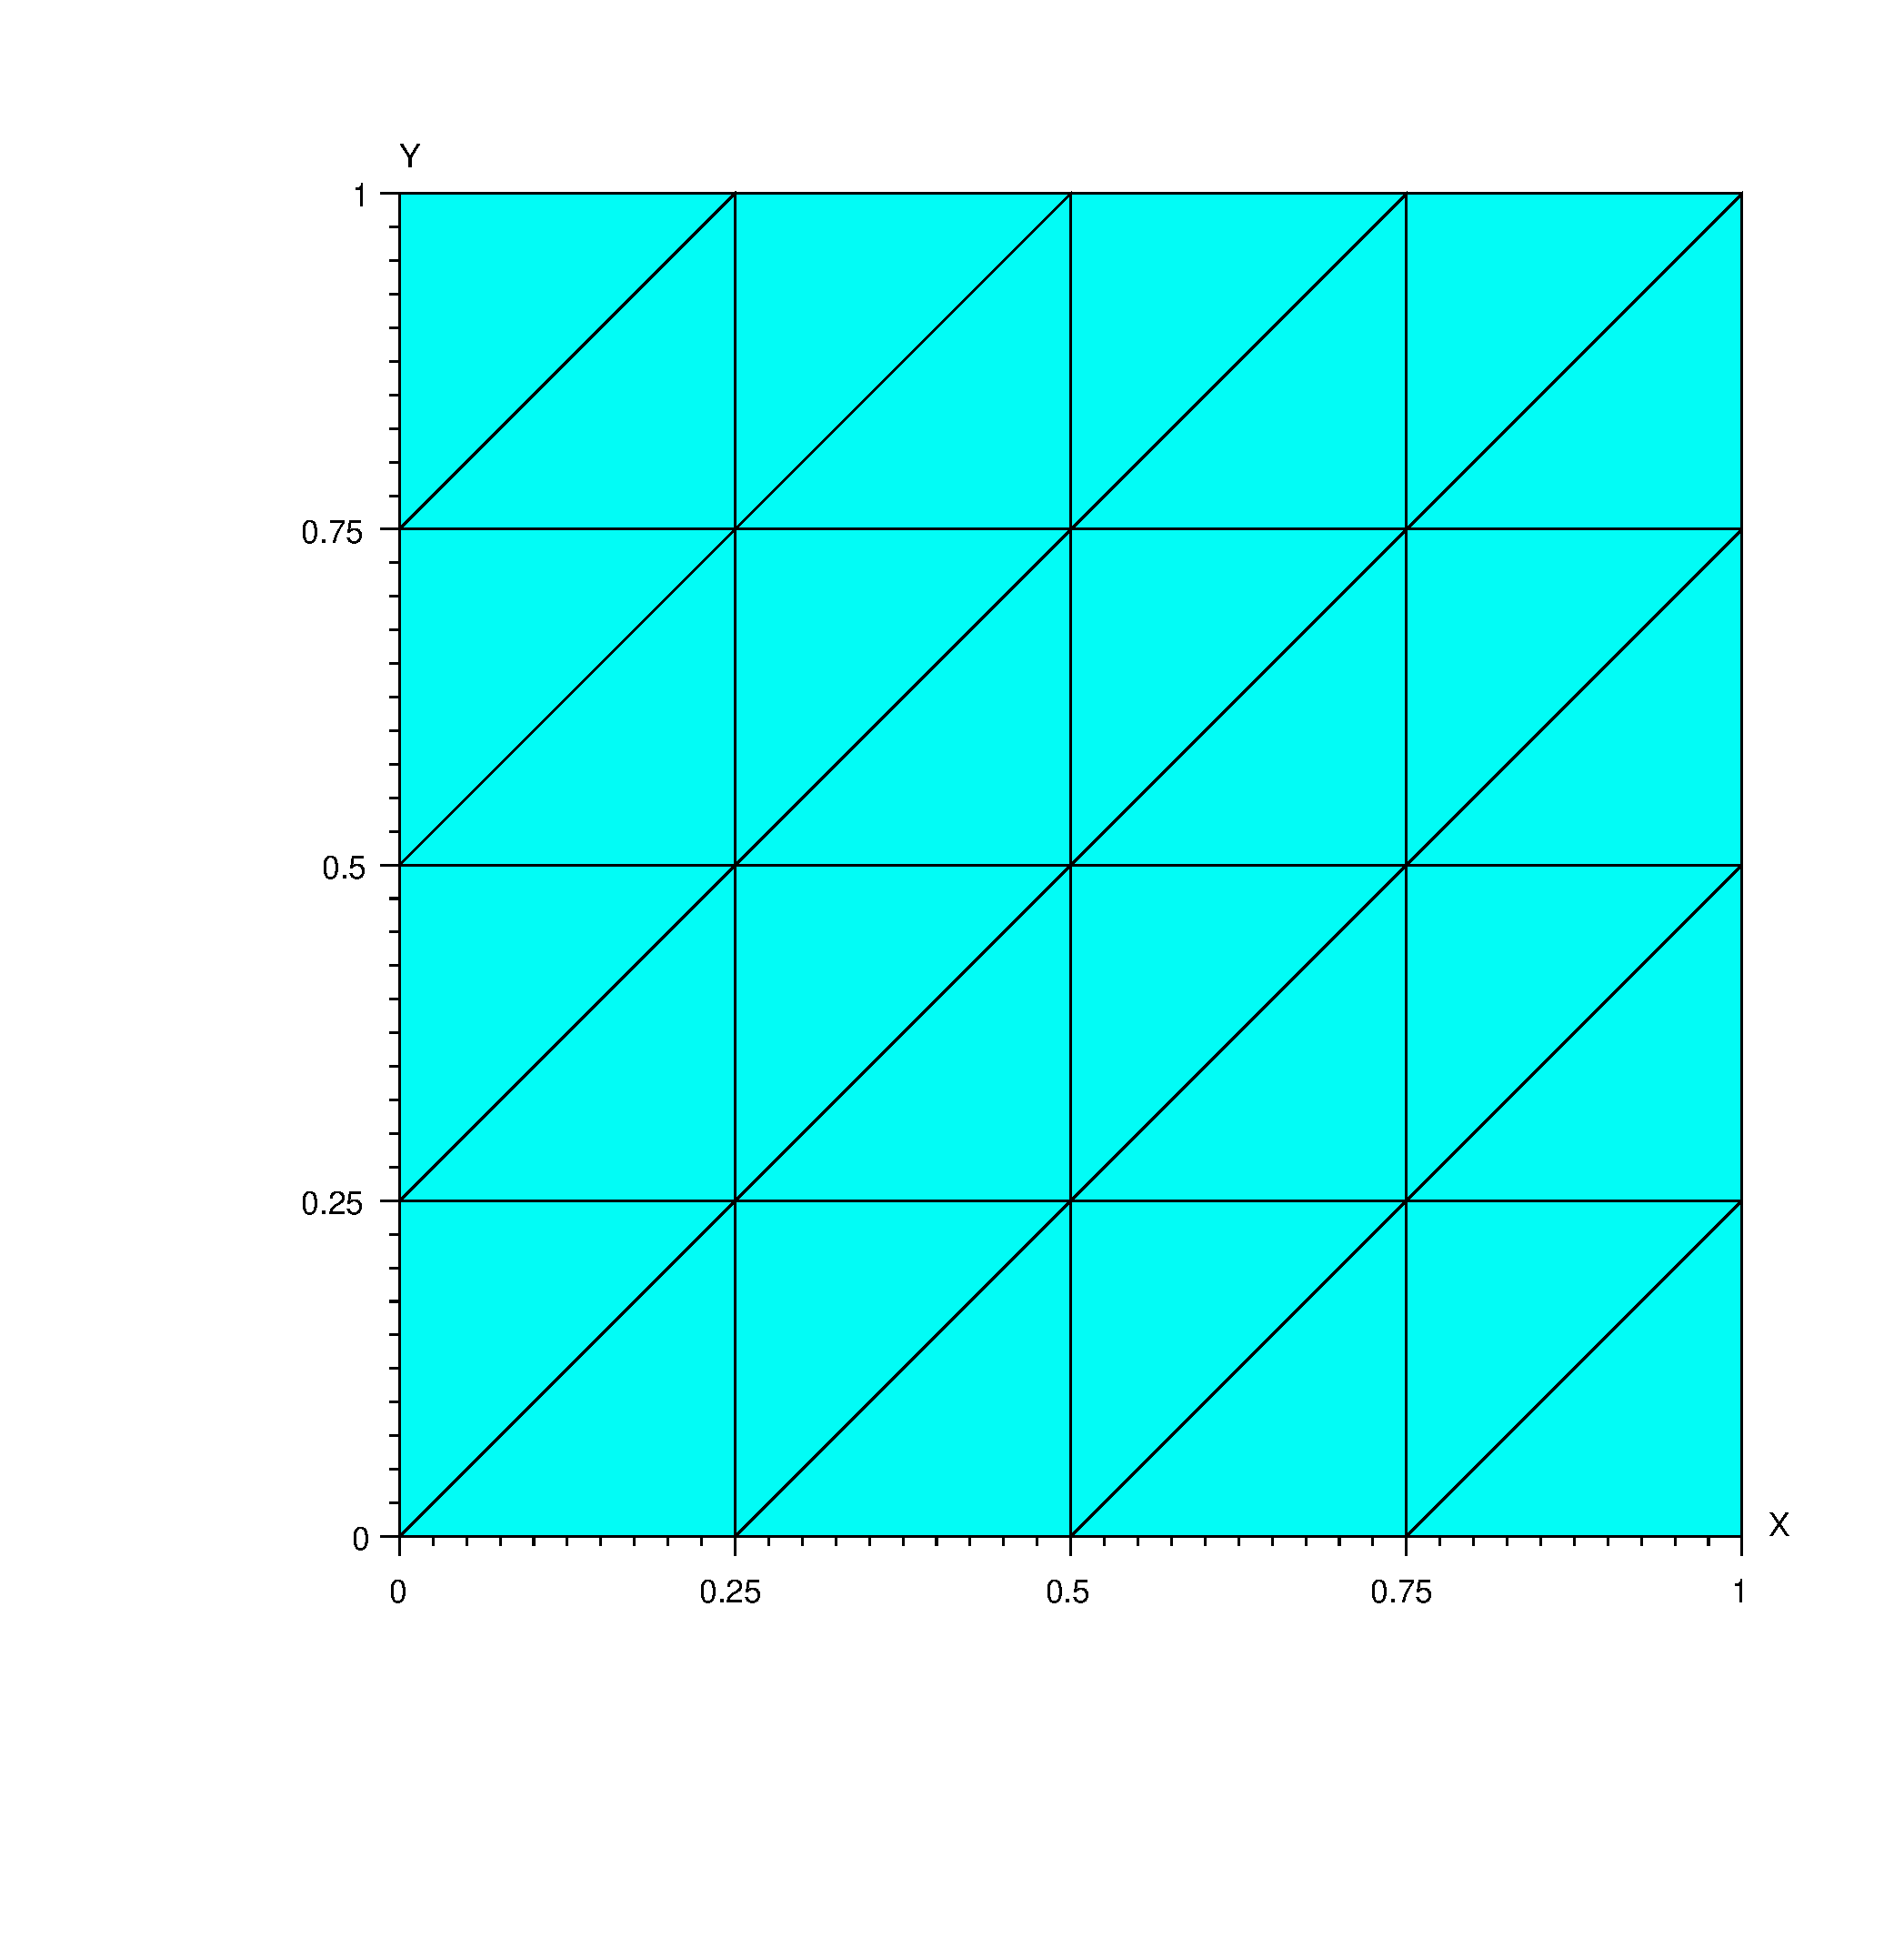
\includegraphics{SquareMesh0.pdf}}
\\[-0.5in]
\hspace{0.45in} \resizebox{!}{0.05\textheight}{$\Downarrow$}
\\[-0.2in]
\resizebox{!}{0.5\textheight}{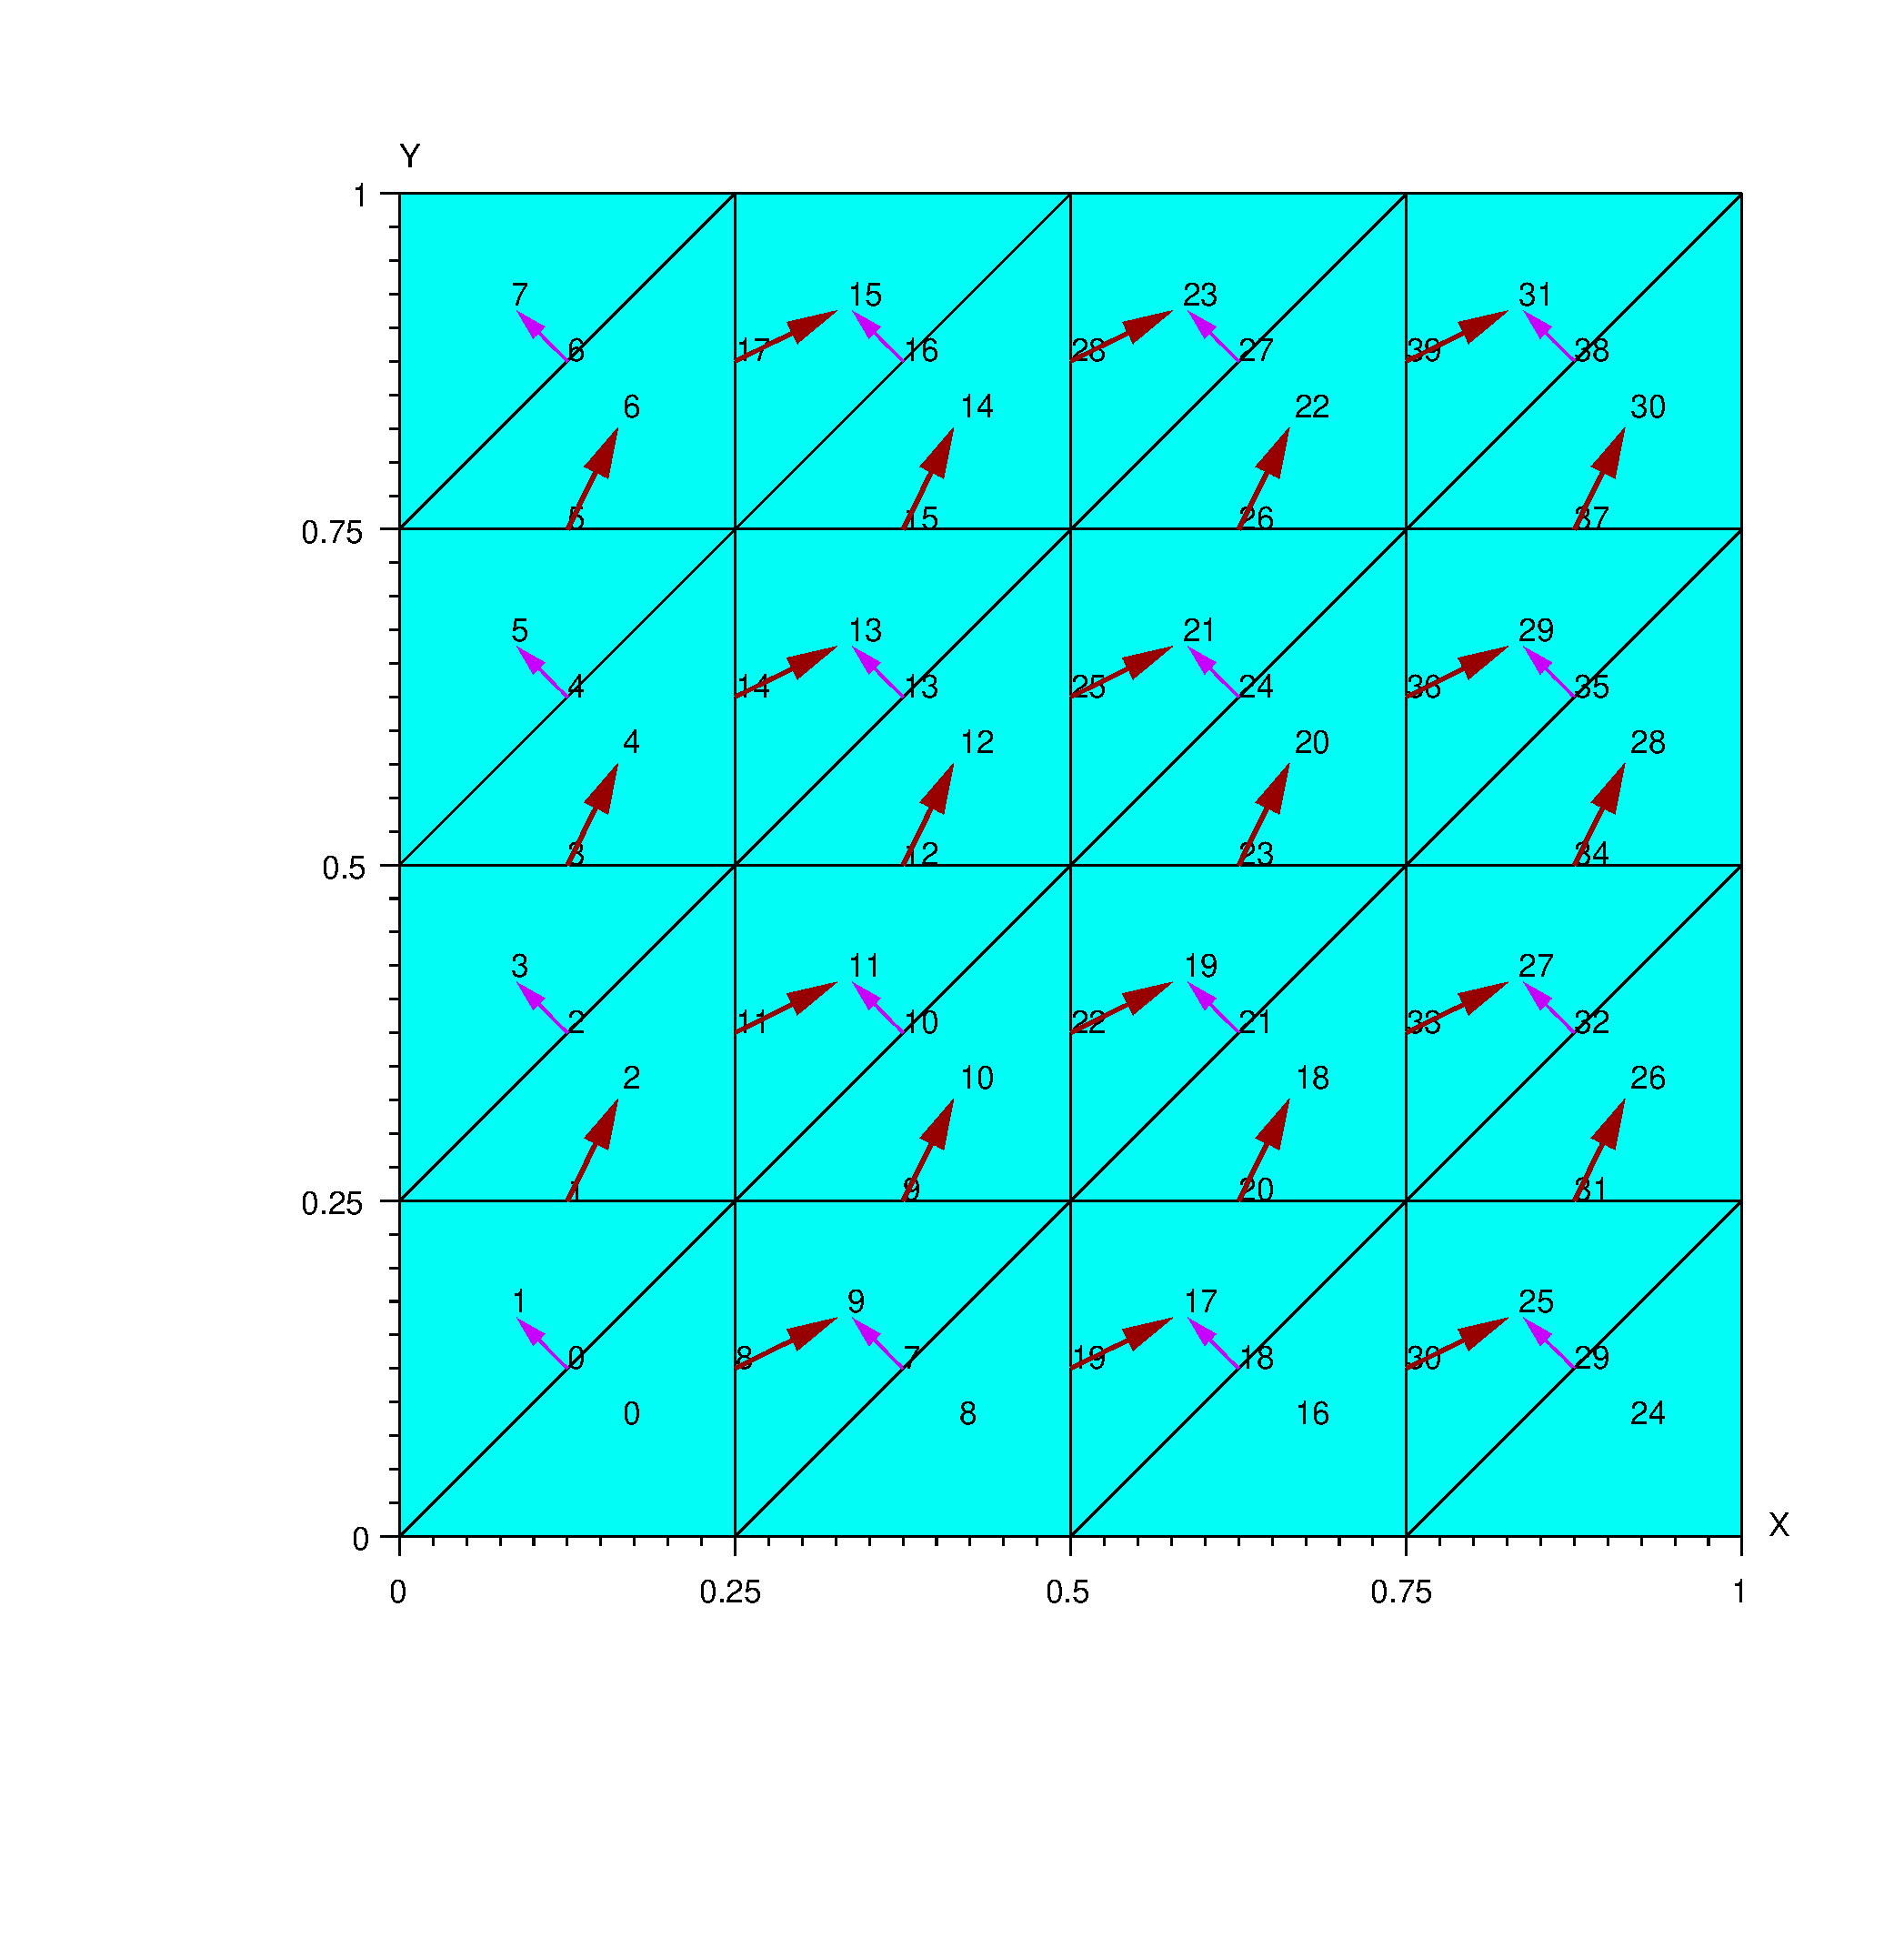
\includegraphics{SquareMesh1.pdf}}
\end{tabular}
\caption{The usual assignment of RWG basis functions 
         to an input surface mesh.
         Integers inside panels denote panel indices.
         Indices lying atop edges denote RWG basis-function indices.
         Arrows indicate directions of current flow.
        } 
\label{NoStraddlerFigure}
\end{center}
\end{figure}
%####################################################################%
To remedy this difficulty, \lss automatically
adds \textit{straddlers} to the surface meshes
specified to the code in geometries involving
extended surfaces. 
This is illustrated in Figure \ref{StraddlerFigure}.
%####################################################################%
\begin{figure}
\begin{center}
\resizebox{\textwidth}{!}{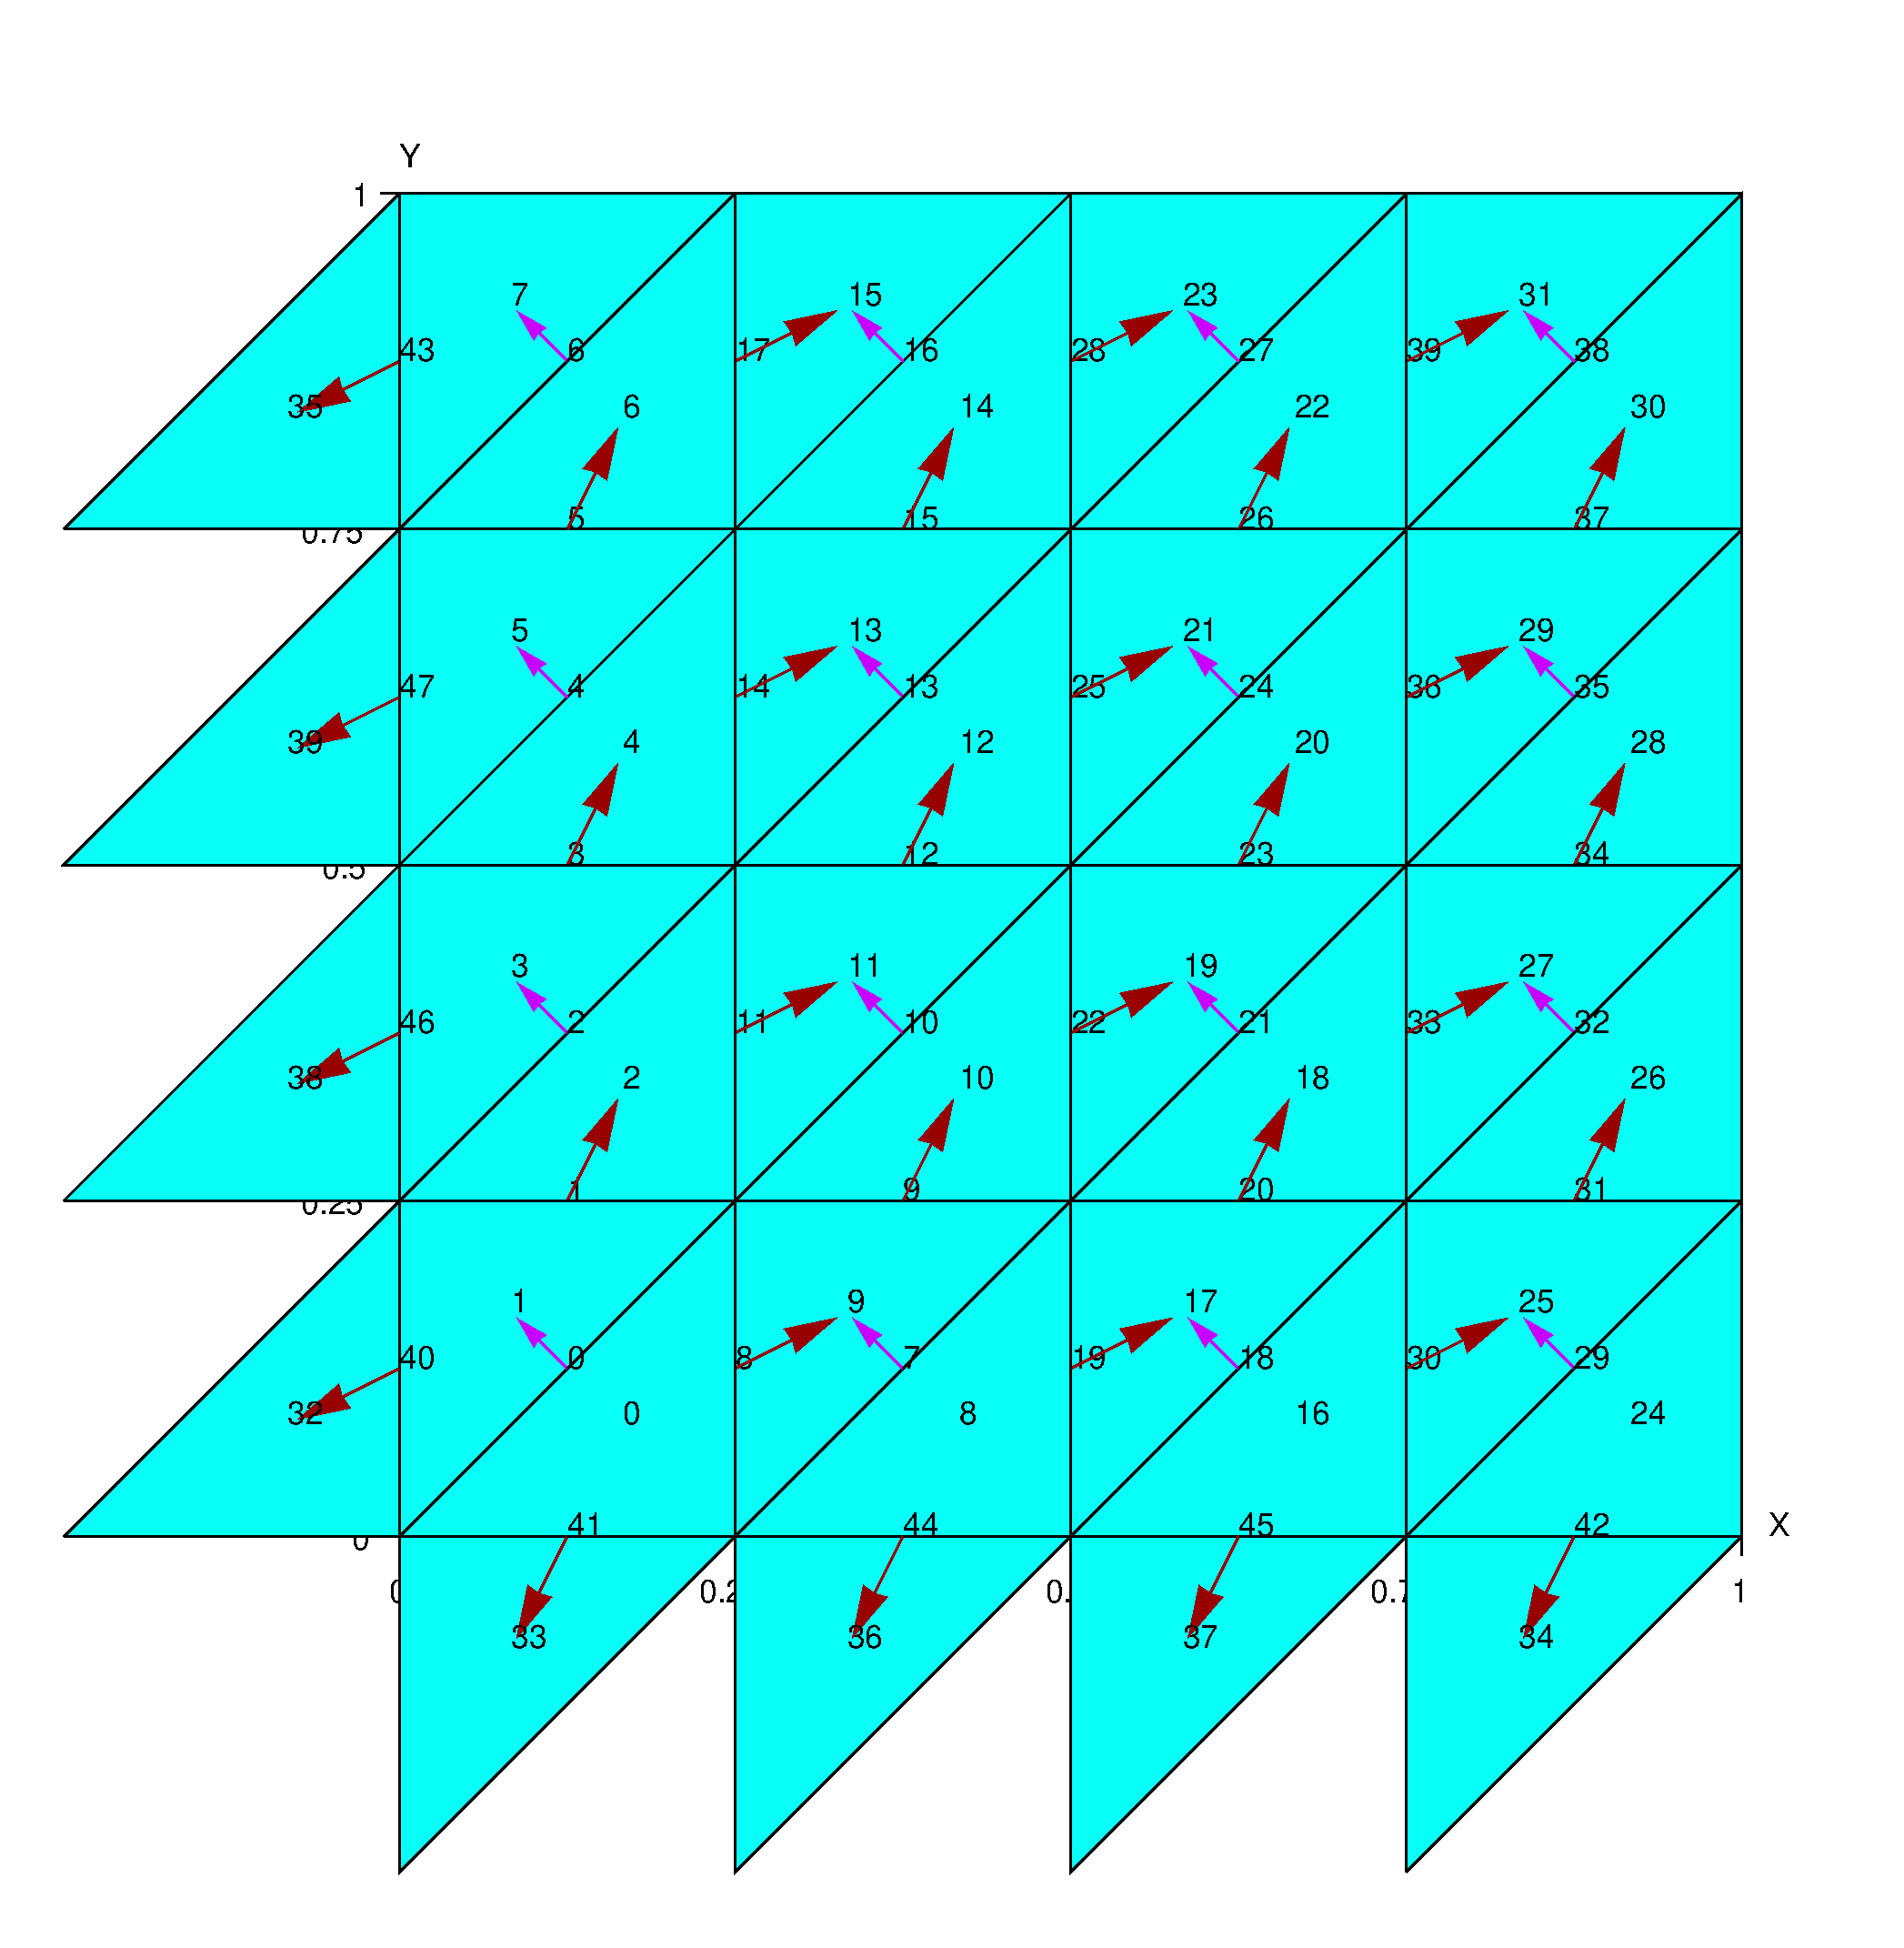
\includegraphics{SquareMesh2.pdf}}
\caption{Straddlers. 
         Integers inside panels denote panel indices.
         Indices lying atop edges denote RWG basis-function indices.
         Arrows indicate directions of current flow.}
\label{StraddlerFigure}
\end{center}
\end{figure}
%####################################################################%

%=================================================
%=================================================
%=================================================
\subsection{Evaluation of surface currents within the unit cell}

When evaluating the $\vb K$ and $\vb N$ surface-current 
distributions at panels that border the upper or right edges 
of the unit-cell mesh, we have to be careful to account for the 
contribution of straddlers. 

For example, consider evaluating the electric surface current at 
oints $\vb x$ inside panel $\mc P_{24}$ in Figure \ref{StraddlerFigure}.
There are three RWG basis functions that contribute to the current
at this point: the functions associated with edges 29 and 42,
and the periodic image of the function associated with edge 40.
Thus we compute
%====================================================================%
$$ \vb K(\vb x) 
   =   k_{29} \vb b_{29}(\vb x) + k_{42} \vb b_{42}(\vb x) 
     + e^{i \KB \cdot \vb L_1} k_{40} \vb b_{40}(\vb x-\vb L_1)
$$
%====================================================================%
where $\vb L_1$ is the lattice basis vector through which we
translate points in panel 32 to yield points in panel 24.
[In this case we have $\vb L_1=(1,0).$]

%=================================================
%=================================================
%=================================================
\subsection{Relations between BEM matrix elements}

Looking at Figure \ref{StraddlerFigure}, it seems 
obvious that BEM matrix elements between the pair of 
basis functions
$\{\vb b_2, \vb b_{24}\}$ will be identical to those
between the pair 
$\{\vb b_4, \vb b_{27}\}$. (This much would be 
true even if we \textit{weren't} talking about
periodic geometries.)

Slightly less obvious is that matrix elements between
the pair $\{\vb b_6, \vb b_{18}\}$ will \textit{also}
be related to matrix elements between the above two
pairs---in fact, the elements will be \textit{identical}
for $\KB=0$ and will differ by only a phase factor
for $\KB\ne 0$. Let's now derive this relationship.

Let $\vb L$ be a lattice vector and 
let 
$\{\vb b_{\alpha}, \vb b_{\beta}\}$
and 
$\{\vb b_{\alpha^\prime}, \vb b_{\beta^\prime}\}$ 
be two pairs of RWG basis functions for which the 
displacement between centroids differs by $\vb L$.
That is, we have 
$$ \vb x_{0\beta}-\vb x_{0\alpha}
   =
   \vb x_{0\beta^\prime}-\vb x_{0\alpha^\prime} + \vb L
$$
where e.g. $\vb x_{0\beta}$ denotes the centroid of 
the support of $\vb b_\beta$.
Examples of basis-function pairs in the mesh of 
Figure \ref{StraddlerFigure} for which this condition
is satisfied include
$$\begin{array}{lclclclclcl}
  (\alpha,\beta)&=&(4,27),  
  &\qquad
  (\alpha^\prime,\beta^\prime)&=&(6,18), 
  &\qquad
  \vb L &=& (0,1)
\\[5pt]
  (\alpha,\beta)&=&(0,32),
  &\qquad
  (\alpha^\prime,\beta^\prime)&=&(7,2), 
  &\qquad
  \vb L &=& (1,0).
  \end{array}
$$

%=================================================
%=================================================
%=================================================
\subsection{Assembly of BEM matrix blocks}

For a geometry in which the unit cell contains $N$ 
surfaces, the BEM matrix at Bloch wavevector $\KB$ 
has the structure
%====================================================================%
\numeq{BlockMatrixStructure}
{ \vb M(\KB)
 =\left(\begin{array}{cccc}
  \vb T_1(\KB)    & \vb U_{12}(\KB) & \cdots & \vb U_{1N}(\KB) \\[3pt]
  \vb U_{21}(\KB) & \vb T_2(\KB)    & \cdots & \vb U_{2N}(\KB) \\[3pt]
  \vdots          & \vdots          & \ddots & \vdots      \\[3pt]
  \vb U_{N1}(\KB) & \vb U_{N2}(\KB) & \cdots & \vb T_{N}(\KB)
  \end{array}\right)
}
%====================================================================%
where $\vb U_{mn}$ describes the interaction of surfaces $m$
and $n$ and $\vb T_m$ describes the self-interaction of
surface $m$.

\subsubsection*{Off-diagonal blocks}

The off-diagonal blocks have the structure

%--------------------------------------------------------------------%
\begin{align}
\vb U_{mn}(\KB)
 =   &\vb U_{mn}\supt{00}
\label{UmnDecomposition}\\
   & + e^{ i \KB \cdot \vb L_1} \vb U_{mn}^{+0}
     + e^{-i \KB \cdot \vb L_1} \vb U_{mn}^{-0}
\nn
   & + e^{ i \KB \cdot \vb L_2} \vb U_{mn}^{0+}
     + e^{-i \KB \cdot \vb L_2} \vb U_{mn}^{0-}
\nn
   & + e^{ i \KB \cdot (\vb L_1+\vb L_2)} \vb U_{mn}^{++}
     + e^{-i \KB \cdot (\vb L_1+\vb L_2)} \vb U_{mn}^{--}
\nn
   & + e^{ i \KB \cdot (\vb L_1-\vb L_2)} \vb U_{mn}^{+-}
     + e^{-i \KB \cdot (\vb L_1-\vb L_2)} \vb U_{mn}^{-+}
\nn
   & + \vb U_{mn}\supt{AB9}(\KB).
\nonumber
\end{align}
%--------------------------------------------------------------------%
In this equation, $\vb U_{mn}^{\sigma \sigma^\prime}$ is the usual 
(non-periodic) matrix describing the interaction of surface $m$ 
with a \textit{displaced} copy of surface $n$; the displacement 
is through displacement vector $\sigma \vb L_1 + \sigma^\prime \vb L_2$
where $\sigma,\sigma^\prime \in \{-1,0,1\}.$ 
On the other hand, $\vb U_{mn}\supt{AB9}$ represents the interaction
of surface $m$ with the infinite set of Bloch-phased 
and displaced copies of surface $n$ \textit{excluding} the contribution
of the innermost 9 grid cells (``AB9'' stands for ``all but 9.'')

The point of the decomposition (\ref{UmnDecomposition}) is that 
the matrix blocks $\vb U_{mn}^{\sigma\sigma^\prime}$ are 
\textit{independent of $\KB$} and hence need only be computed 
once at a given angular frequency, after which they may be reused
for any number of calculations at different points in the Brillouin
zone. 

In {\sc scuff-em}, the $\KB$-independent matrix blocks 
$\vb U_{mn}^{\sigma\sigma^\prime}$ are computed using the ordinary
algorithm for assembling the blocks of the BEM matrix 
for compact (non-periodic) geometries. An advantage of this
is that singular integrals involving pairs of panels in
adjacent cells with common edges or vertices are handled
correctly using singular-integral evaluation techniques
present in {\sc scuff-em}.
For example, in the mesh of Figure \ref{StraddlerFigure},
panel 1 of the unit-cell mesh has a common edge 
with panel 24 of the $(-1,0)$ mesh image.

\subsubsection*{Transposes of off-diagonal blocks}

Once we have computed the 
$\vb U_{mn}^{\sigma\sigma^\prime}$ blocks for the $mn$ block of 
the BEM, we may re-use them to compute the $nm$ block, as follows 
based on equation (\ref{PBCMatrixTranspose}):
%--------------------------------------------------------------------%
\begin{align}
\vb U_{nm}(\KB) 
=  &\Big[\vb U_{mn}(-\KB)\Big]^T 
\\
=  &\Big[\vb U_{mn}\supt{00}]^T
\\
   & + e^{ -i \KB \cdot \vb L_1} \Big[\vb U_{mn}^{+0}\Big]^T
     + e^{  i \KB \cdot \vb L_1} \Big[\vb U_{mn}^{-0}\Big]^T
\nn
   & + e^{ -i \KB \cdot \vb L_2} \Big[\vb U_{mn}^{0+}\Big]^T
     + e^{ +i \KB \cdot \vb L_2} \Big[\vb U_{mn}^{0-}\Big]^T
\nn
   & + e^{ -i \KB \cdot (\vb L_1+\vb L_2)} \Big[\vb U_{mn}^{++}\Big]^T
     + e^{ +i \KB \cdot (\vb L_1+\vb L_2)} \Big[\vb U_{mn}^{--}\Big]^T
\nn
   & + e^{ -i \KB \cdot (\vb L_1-\vb L_2)} \Big[\vb U_{mn}^{+-}\Big]^T
     + e^{ +i \KB \cdot (\vb L_1-\vb L_2)} \Big[\vb U_{mn}^{-+}\Big]^T
\nn
   & + \vb U_{nm}\supt{AB9}(\KB).
\nonumber
\end{align}
%--------------------------------------------------------------------%

\subsubsection*{Diagonal blocks}

For the diagonal blocks there are additional symmetries, e.g.
$ \vb T_{m}^{--} = \Big[\vb T_{m}^{++}\Big]^T, $
and hence the equivalent of (\ref{UmnDecomposition}) reads 
%--------------------------------------------------------------------%
\begin{align}
\vb T_{m}(\KB)
 =   &\vb T_{m}\supt{00}
\label{TmDecomposition}\\
   & + e^{ i \KB \cdot \vb L_1} \vb T_{m}^{+0}
     + e^{-i \KB \cdot \vb L_1} \Big[\vb T_{m}^{+0}\Big]^T
\nn
   & + e^{ i \KB \cdot \vb L_2} \vb T_{m}^{0+}
     + e^{-i \KB \cdot \vb L_2} \Big[\vb T_{m}^{0+}\Big]^T
\nn
   & + e^{ i \KB \cdot (\vb L_1+\vb L_2)} \vb T_{m}^{++}
     + e^{-i \KB \cdot (\vb L_1+\vb L_2)} \Big[ \vb T_{m}^{++}\Big]^T
\nn
   & + e^{ i \KB \cdot (\vb L_1-\vb L_2)} \vb T_{m}^{+-}
     + e^{-i \KB \cdot (\vb L_1-\vb L_2)} \Big[ \vb T_{m}^{+-}\Big]^T
\nn
   & + \vb T_{m}\supt{AB9}(\KB).
\nonumber
\end{align}
%--------------------------------------------------------------------%
Hence to assemble $\vb T(\KB)$ we need only compute and
store 5 $\KB$-independent blocks $\vb T^{\sigma \sigma^\prime}$
instead of the 9 $\KB$-independent blocks required to assemble
$\vb U(\KB)$.

\subsubsection*{Assessing the connectivity of regions}

An important subtlety in the BEM matrix assembly for dielectric
geometries treated by the PMCHWT formulation concerns the question
of the ``extendedness'' or connectivity of material regions.

In general, the surfaces $m,n$ whose interaction is described
by the $\vb T_m$ and $\vb U_{mn}$ blocks in (\ref{BlockMatrixStructure}) 
will interact through one or two common \textit{regions} (material media).
(More specifically, $\vb T$ blocks will typically involve two common
regions, while $\vb U$ blocks will typically involve one common region.)

The BEM matrix elements




\appendix

\include{IndexNotationAppendix} 
\newpage
\section{Notation for Spherical Helmholtz Solutions}
\label{SphericalHelmoltzAppendix}

The spherical-multipole computations of 
Section \ref{SphericalMultipoleMatrixElementSection}
make reference to standard results in the theory of 
scattering from spherical geometries.\footnote{As discussed 
at length in Morse and Feschbach, Jackson, and other 
standard texts.} Here is a summary of the notation 
and conventions I use for this material.

%%%%%%%%%%%%%%%%%%%%%%%%%%%%%%%%%%%%%%%%%%%%%%%%%%%%%%%%%%%%%%%%%%%%%%
%%%%%%%%%%%%%%%%%%%%%%%%%%%%%%%%%%%%%%%%%%%%%%%%%%%%%%%%%%%%%%%%%%%%%%
%%%%%%%%%%%%%%%%%%%%%%%%%%%%%%%%%%%%%%%%%%%%%%%%%%%%%%%%%%%%%%%%%%%%%%
\subsection{Vector Helmholtz Solutions}

I use the symbols $\vb M(\vb r)$, $\vb N(\vb r)$ to denote 
divergenceless vector-valued functions whose components each 
separately satisfy the Helmholtz equation:
$$
 \nabla \cdot 
 \left\{ \begin{array}{c} \vb M \\ \vb N \end{array} \right\} 
  = 0 
$$
and
\begin{align*}
%%%%%%%%%%%%%%%%%%%%%%%%%
 \Big[\nabla^2 + k^2 \Big] 
 \left\{ \begin{array}{c} \vb M \\ \vb N \end{array} \right\} 
 &= 0 
 \qquad \text{real frequency}
  \\[8pt]
%%%%%%%%%%%%%%%%%%%%%%%%%
%%%%%%%%%%%%%%%%%%%%%%%%%
 \Big[\nabla^2 - \kappa^2 \Big] 
 \left\{ \begin{array}{c} \vb M \\ \vb N \end{array} \right\} 
 &= 0 
 \qquad \text{imaginary frequency}.
%%%%%%%%%%%%%%%%%%%%%%%%%%
\end{align*}
%
\subsubsection*{Vector Helmholtz Solutions for Spherical Geometries}
For spherical geometries we take $\vb M$ to have the form
%
\numeq{Mlm} {\vb M_{lm}(r,\theta,\phi) = R_l(r) \vb X_{lm}(\theta,\phi) }
%
where\footnote{Note that my $\vb X$ function is $-i$ times Jackson's $\vb X$
function.}
$$
 \vb X_{lm}(\theta, \phi)
=-(\vb r \times \nabla) Y_{lm}(\theta,\phi)
\equiv \frac{1}{\sqrt{l(l+1)}}
   \Big[ \frac{im}{\sin\theta} Y_{lm} \hat{\boldsymbol{\theta}}
         -\pard{Y_{lm}}{\theta} \hat{\boldsymbol{\varphi}}
   \Big]
$$
and where the radial function is a spherical Bessel function whose
precise form depends on whether we are at real or imaginary frequency and 
whether we want a solution that is well-behaved at the origin (the 
``interior'' solution) or well-behaved at infinity (the ``exterior'' 
solution):
%%%%%%%%%%%%%%%%%%%%%%%%%%%%%%%%%%%%%%%%%%%%%%%%%%
%%%%%%%%%%%%%%%%%%%%%%%%%%%%%%%%%%%%%%%%%%%%%%%%%%
%%%%%%%%%%%%%%%%%%%%%%%%%%%%%%%%%%%%%%%%%%%%%%%%%%
\begin{center}
\textbf{Forms of the radial function $R_l(r):$}

\medskip

\begin{tabular}{|c|c|c|}  \hline
                               & \textbf{Interior} & \textbf{Exterior}   \\ \hline
\textbf{Real frequency}        & $j_l(kr)$         & $j_l(kr) +iy_l(kr)$ \\ \hline
\textbf{Imaginary frequency}   & $i_l(\kappa r)$   & $k_l(\kappa r)    $ \\ \hline
\end{tabular}
\end{center}
\medskip

%%%%%%%%%%%%%%%%%%%%%%%%%%%%%%%%%%%%%%%%%%%%%%%%%%
%%%%%%%%%%%%%%%%%%%%%%%%%%%%%%%%%%%%%%%%%%%%%%%%%%
%%%%%%%%%%%%%%%%%%%%%%%%%%%%%%%%%%%%%%%%%%%%%%%%%%

\noindent Next, $\vb N$ is defined in terms of $\vb M$ according to
%
\numeq{NDef}
{\vb N_{lm}
   \equiv 
   \begin{cases} 
     %%%%%%%%%%%%%%%%%%%%%%%%%%%%%%%%%%%%%%%%%%%%%%%%%%
     \displaystyle{ -\frac{1}{ik} \nabla \times \vb M_{lm} }, 
      \qquad &\text{real frequency} \\[10pt]
     %%%%%%%%%%%%%%%%%%%%%%%%%%%%%%%%%%%%%%%%%%%%%%%%%%
     \displaystyle{ \quad \frac{1}{\kappa} \nabla \times \vb M_{lm} },
      \qquad &\text{imaginary frequency}.
     \end{cases}
}
%
This definition for $\vb N,$ together with the facts that $\vb M$ 
has vanishing divergence and satisfies the vector Helmholtz equation,
lead to the reciprocal curl identities:
%
$$\nabla \times \vb N_{lm}
   \equiv 
   \begin{cases} 
     %%%%%%%%%%%%%%%%%%%%%%%%%%%%%%%%%%%%%%%%%%%%%%%%%%
     \displaystyle{ +ik \vb M_{lm} }, 
      \qquad &\text{real frequency} \\[10pt]
     %%%%%%%%%%%%%%%%%%%%%%%%%%%%%%%%%%%%%%%%%%%%%%%%%%
     \displaystyle{ -\kappa \vb M_{lm} },
      \qquad &\text{imaginary frequency}.
     \end{cases}
$$

%%%%%%%%%%%%%%%%%%%%%%%%%%%%%%%%%%%%%%%%%%%%%%%%%%%%%%%%%%%%%%%%%%%%%%
%%%%%%%%%%%%%%%%%%%%%%%%%%%%%%%%%%%%%%%%%%%%%%%%%%%%%%%%%%%%%%%%%%%%%%
%%%%%%%%%%%%%%%%%%%%%%%%%%%%%%%%%%%%%%%%%%%%%%%%%%%%%%%%%%%%%%%%%%%%%%
\subsubsection*{Spherical Components of $\vb M$ and $\vb N$}
Explicit expression for the components of $\vb M$ and $\vb N$ are 
%====================================================================%
\begin{align}
%--------------------------------------------------------------------%
 \vb M_{lm}
&= \frac{1}{\sqrt{l(l+1)}}
   R_l\bigg[ +\frac{im}{\sin\theta} Y_{lm}\hat{\boldsymbol{\theta}} 
                   -\pard{Y_{lm}}{\theta}\hat{\boldsymbol{\varphi}}
         \bigg]
%--------------------------------------------------------------------%
\intertext{(valid at real or imaginary frequency)}
%--------------------------------------------------------------------%
 \vb N_{lm}
&= \frac{1}{-ik\sqrt{l(l+1)}}
   \bigg[\frac{l(l+1)}{r}R_l Y_{lm}\vbhat{r}
         +\Big(\frac{R_l}{r} + \pard{R_l}{r}\Big)
          \Big\{\pard{Y_{lm}}{\theta} \hat{\boldsymbol{\theta}}
              +\frac{im}{\sin\theta} Y_{lm} \hat{\boldsymbol{\varphi}}
          \Big\} 
   \bigg]
\intertext{(at real frequency)}
%--------------------------------------------------------------------%
 \vb N_{lm}
&= \frac{1}{\kappa\sqrt{l(l+1)}}
   \bigg[\frac{l(l+1)}{r}R_l Y_{lm}\vbhat{r}
         +\Big(\frac{R_l}{r} + \pard{R_l}{r}\Big)
          \Big\{\pard{Y_{lm}}{\theta} \hat{\boldsymbol{\theta}}
              +\frac{im}{\sin\theta} Y_{lm} \hat{\boldsymbol{\varphi}}
          \Big\} 
   \bigg]
%--------------------------------------------------------------------%
\end{align}
at imaginary frequency. Here $R_l$ is one of the functions in the table above.

%%%%%%%%%%%%%%%%%%%%%%%%%%%%%%%%%%%%%%%%%%%%%%%%%%%%%%%%%%%%%%%%%%%%%%
%%%%%%%%%%%%%%%%%%%%%%%%%%%%%%%%%%%%%%%%%%%%%%%%%%%%%%%%%%%%%%%%%%%%%%
%%%%%%%%%%%%%%%%%%%%%%%%%%%%%%%%%%%%%%%%%%%%%%%%%%%%%%%%%%%%%%%%%%%%%%
\subsubsection*{Hat/Wedge Notation}
%
I will use the notation $\MInt,\NInt$ and $\MExt,\NExt$ to refer 
respectively to the ``interior'' and ``exterior'' solutions. 
(Mnemonic: The $\vee$ symbol atop $\vb M$ or $\vb N$ suggests that 
the quantity in question is radiating \textit{outward} into space, 
as appropriate for an exterior solution.)
Thus
%====================================================================%
\begin{align}
%--------------------------------------------------------------------%
   \left\{\begin{array}{c} 
     \MInt_{lm}(r, \theta, \varphi) \\[5pt] 
     \MExt_{lm}(r, \theta, \varphi) 
   \end{array}\right\}
&=\frac{1}{\sqrt{l(l+1)}}
   \left\{\begin{array}{c} 
     j_l(kr) \\[5pt] 
     j_l(kr)+iy_l(kr)
   \end{array}\right\}
   \vb X_{lm}(\theta, \varphi)
  \label{MDefReal} 
\intertext{at real frequency, and}
%--------------------------------------------------------------------%
   \left\{\begin{array}{c} 
     \MInt_{lm}(r, \theta, \varphi) \\[5pt] 
     \MExt_{lm}(r, \theta, \varphi) 
   \end{array}\right\}
&=\frac{1}{\sqrt{l(l+1)}}
   \left\{\begin{array}{c} 
     i_l(\kappa r) \\[5pt] 
     k_l(\kappa r)
   \end{array}\right\}
   \vb X_{lm}(\theta, \varphi)
  \label{MDefImag}
%--------------------------------------------------------------------%
\end{align}
at imaginary frequency.

Notwithstanding the resemblance of my $\wedge$ and $\vee$ adornments to 
Slavic diacritic marks, there is no danger of ambiguity here, as in 
this particular document I will resist the temptation to write in either 
the Serbo-Croatian \textit{or} Bosnian dialects. (This means I will
have to forego all my best jokes, but whaddya gonna do.)
%====================================================================%

%%%%%%%%%%%%%%%%%%%%%%%%%%%%%%%%%%%%%%%%%%%%%%%%%%%%%%%%%%%%%%%%%%%%%%
%%%%%%%%%%%%%%%%%%%%%%%%%%%%%%%%%%%%%%%%%%%%%%%%%%%%%%%%%%%%%%%%%%%%%%
%%%%%%%%%%%%%%%%%%%%%%%%%%%%%%%%%%%%%%%%%%%%%%%%%%%%%%%%%%%%%%%%%%%%%%
\subsubsection*{Compound Indices}

I will frequently use $\alpha=(lm)$ and $\beta=(l^\prime m^\prime)$ 
as compound indices in summations over spherical multipole indices,
i.e. 
$$ \sum_{l=0}^{l\subt{max}} \sum_{m=-l}^{l}
   \sum_{l^\prime}^{l\subt{max}^\prime} \sum_{m=-l^\prime}^{l^\prime}
   \Big\{ \cdots \Big\}_{lm} 
   \Big\{ \cdots \Big\}_{l^\prime m^\prime} 
\qquad \longrightarrow \qquad 
   \sum_{\alpha=0}^{N_\alpha-1}
   \sum_{\beta=0}^{N_\beta-1}
   \Big\{ \cdots \Big\}_{\alpha} 
   \Big\{ \cdots \Big\}_{\beta}
$$
where 
$\alpha = l^2 + l + m$,
$N_\alpha=(l\subt{max}+1)^2.$ 

%%%%%%%%%%%%%%%%%%%%%%%%%%%%%%%%%%%%%%%%%%%%%%%%%%%%%%%%%%%%%%%%%%%%%%
%%%%%%%%%%%%%%%%%%%%%%%%%%%%%%%%%%%%%%%%%%%%%%%%%%%%%%%%%%%%%%%%%%%%%%
%%%%%%%%%%%%%%%%%%%%%%%%%%%%%%%%%%%%%%%%%%%%%%%%%%%%%%%%%%%%%%%%%%%%%%
\subsection{Translation Matrices}

The translation matrices relate exterior Helmholtz solutions 
about one origin to interior Helmholtz solutions about a 
different origin. Let the former origin be $\vb x_0$ and the latter
origin be $\vb x_0^\prime.$ Then the relevant relations read
%====================================================================%
\begin{subequations}
\begin{align*}
 \Big|\MExt_\alpha(\vb x - \vb x_0^\prime) \Big\rangle
&= \sum_{\beta} 
     A_{\alpha\beta} \Big|\MInt_\beta(\vb x-\vb x_0) \Big\rangle 
    +B_{\alpha\beta} \Big|\NInt_\beta(\vb x-\vb x_0) \Big\rangle
\\
%--------------------------------------------------------------------%
 \Big|\NExt_\alpha(\vb x - \vb x_0^\prime) \Big\rangle
&= \sum_{\beta} 
    -B_{\alpha\beta} \Big|\MInt_\beta(\vb x-\vb x_0) \Big\rangle 
    +A_{\alpha\beta} \Big|\NInt_\beta(\vb x-\vb x_0) \Big\rangle.
\end{align*}
\label{TranslationMatrixDefinition}
\end{subequations}
%====================================================================%
where the translation matrices $\{A_{\alpha\beta}, B_{\alpha\beta}\}$
depend on $k$ and on the separation
vector connecting the two origins.

The bra-ket notation in (\ref{TranslationMatrixDefinition})
obscures the need to rotate the spherical components of the
vector functions $\vb M$ and $\vb N$, which is actually fine  
as long as we only ever need to talk about inner products
of $\vb M$ and $\vb N$ with other vector-valued functions.
In particular, we have
\begin{align*}
 \big\langle \vb f \big| \MExt_\alpha \Big>
&= \sum_{\beta } \Big\{ 
   A_{\alpha\beta} \big\langle \vb f \big| \MInt_\beta \big>
  +B_{\alpha\beta} \big\langle \vb f \big| \NInt_\beta \big>
  \Big\} 
\\
 \big\langle \vb f \big| \NExt_\alpha \Big>
&= \sum_\beta \Big\{ 
   -B_{\alpha\beta} \big\langle \vb f \big| \MInt_\beta \big>
   +A_{\alpha\beta} \big\langle \vb f \big| \NInt_\beta \big>.
  \Big\}
\end{align*}
 
%\documentclass[letterpaper]{article}
%%********************************************************
%* latex shortcuts used for libscuff documentation files
%* 
%* homer reid -- 1994--2011
%**************************************************
\usepackage{graphicx}
\usepackage{color}
\usepackage{dsfont}
\usepackage{bbm}
\usepackage{amsmath}
\usepackage{amssymb}
\usepackage{float}
\usepackage{psfrag}
\usepackage{mathdots}
%\usepackage{algorithm}
%\usepackage{algorithmic}
%\usepackage{listings}
\usepackage{array}
\usepackage{url}
\usepackage{arydshln}
\usepackage{fancybox}
\usepackage{fancyvrb}
\usepackage{verbatim}

%--------------------------------------------------
%- boldface greek letters 
%--------------------------------------------------
\newcommand\vbphi{\mathbf{\phi}}
\newcommand\vbPhi{\mathbf{\Phi}}
\newcommand{\vbDelta}{\boldsymbol{\Delta}}
\newcommand{\vbrho}{\boldsymbol{\rho}}
\newcommand{\vbchi}{\boldsymbol{\chi}}

%--------------------------------------------------
%- colors -----------------------------------------
%--------------------------------------------------
\newcommand{\red}[1]{\textcolor{red}{#1}}
\newcommand{\blue}[1]{\textcolor{blue}{#1}}
\newcommand{\green}[1]{\textcolor{green}{#1}}
\newcommand{\atan}{\text{atan}}

%--------------------------------------------------
% general commands
%--------------------------------------------------
\newcommand\Tr{\hbox{Tr }}
\newcommand\sups[1]{^{\hbox{\scriptsize{#1}}}}
\newcommand\supt[1]{^{\hbox{\tiny{#1}}}}
\newcommand\subs[1]{_{\hbox{\scriptsize{#1}}}}
\newcommand\subt[1]{_{\hbox{\tiny{#1}}}}
\newcommand{\nn}{\nonumber \\}
\newcommand{\vb}[1]{\mathbf{#1}}
\newcommand{\numeq}[2]{\begin{equation} #2 \label{#1} \end{equation}}
\newcommand{\pard}[2]{\frac{\partial #1}{\partial #2}}
\newcommand{\pardn}[3]{\frac{\partial^{#1} #2}{\partial #3^{#1}}}
\newcommand{\pf}[2]{\left(\frac{#1}{#2}\right)}
\newcommand{\pp}{{\prime\prime}}
\newcommand{\vbhat}[1]{\vb{\hat #1}}
\newcommand{\mc}[1]{\mathcal{#1}}
\newcommand{\bmc}[1]{\boldsymbol{\mathcal{#1}}}
\newcommand{\mb}[1]{\mathbb{#1}}
\newcommand{\ds}[1]{\displaystyle{#1}}
\newcommand{\primedsum}{\sideset{}{'}{\sum}}
\newcommand{\pan}{\mathcal{P}}

%--------------------------------------------------
%- special libscuff stuff--------------------------
%--------------------------------------------------
\newcommand\ls{{\sc libscuff}}
\newcommand\lss{{\sc libscuff\,}}
\newcommand{\BG}{\boldsymbol{\Gamma}}
\newcommand{\MInt}{\vb{\hat M}}
\newcommand{\NInt}{\vb{\hat N}}
\newcommand{\MExt}{\vb{\check M}}
\newcommand{\NExt}{\vb{\check N}}
\newcommand{\xInt}{\vb{\hat x}}
\newcommand{\xExt}{\vb{\check x}}

%--------------------------------------------------
%-- superscripts for dyadic green's functions 
%--------------------------------------------------
\newcommand{\EEe}{^{\hbox{\tiny{EE}\scriptsize{,$e$}}}}
\newcommand{\MEe}{^{\hbox{\tiny{ME}\scriptsize{,$e$}}}}
\newcommand{\EMe}{^{\hbox{\tiny{EM}\scriptsize{,$e$}}}}
\newcommand{\MMe}{^{\hbox{\tiny{MM}\scriptsize{,$e$}}}}
\newcommand{\EEr}{^{\hbox{\tiny{EE}\scriptsize{,$r$}}}}
\newcommand{\MEr}{^{\hbox{\tiny{ME}\scriptsize{,$r$}}}}
\newcommand{\EMr}{^{\hbox{\tiny{EM}\scriptsize{,$r$}}}}
\newcommand{\MMr}{^{\hbox{\tiny{MM}\scriptsize{,$r$}}}}
\newcommand{\incr}{^{\text{\scriptsize inc},r}}
\newcommand{\incro}{^{\text{\scriptsize inc},r_1}}
\newcommand{\incrt}{^{\text{\scriptsize inc},r_2}}

%%%%%%%%%%%%%%%%%%%%%%%%%%%%%%%%%%%%%%%%%%%%%%%%%%%%%%%%%%%%%%%%%%%%%%
%%%%%%%%%%%%%%%%%%%%%%%%%%%%%%%%%%%%%%%%%%%%%%%%%%%%%%%%%%%%%%%%%%%%%%
%%%%%%%%%%%%%%%%%%%%%%%%%%%%%%%%%%%%%%%%%%%%%%%%%%%%%%%%%%%%%%%%%%%%%%
\newcommand{\MMExt}{\check{\mathcal{M}}}
\newcommand{\MMInt}{\hat{\mathcal{M}}}
\newcommand{\NNExt}{\check{\mathcal{N}}}
\newcommand{\NNInt}{\hat{\mathcal{N}}}
\newcommand{\BMMExt}{\boldsymbol{\check{\mathcal{M}}}}
\newcommand{\BMMInt}{\boldsymbol{\hat{\mathcal{M}}}}
\newcommand{\BNNExt}{\boldsymbol{\check{\mathcal{N}}}}
\newcommand{\BNNInt}{\boldsymbol{\hat{\mathcal{N}}}}
\newpage

%--------------------------------------------------
%- inner products and operator matrix elements  ---
%--------------------------------------------------
\newcommand{\expval}[1]{ \big\langle #1 \big\rangle}
\newcommand{\Expval}[1]{ \Big\langle #1 \Big\rangle}
\newcommand{\inp}[2]{ \big\langle #1 \big| #2 \big\rangle}
\newcommand{\Inp}[2]{ \Big\langle #1 \Big| #2 \Big\rangle}
\newcommand{\INP}[2]{ \bigg\langle #1 \bigg| #2 \Big\rangle}
\newcommand{\vmv}[3]{ \big\langle #1 \big| #2 \big| #3 \big\rangle}
\newcommand{\VMV}[3]{ \Big\langle #1 \Big| #2 \Big| #3 \Big\rangle}

%------------------------------------------------------------
%- shaded box for source code inclusions 
%------------------------------------------------------------
%\definecolor{lightgrey}{rgb}{0.85,0.85,0.85}
%\newcommand{\SourceBox}[1]
% { \begin{mdframed}[backgroundcolor=lightgrey, linewidth=2pt,
%                    tikzsetting={draw=black, line width=2pt,
%                                 dashed, dash pattern= on 5pt off 5pt}] %
%  \begin{verbatim} #1 \end{verbatim} \end{mdframed} \medskip
%}
%\IfFileExists{mdframed.sty}
% { \usepackage{mdframed}
%   \surroundwithmdframed[backgroundcolor=lightgrey, linewidth=2pt,
%                         framemethod=tikz,
%                         skipabove=10pt,
%                         skipbelow=10pt,
%                         tikzsetting={draw=black, line width=2pt,
%                                      dashed, dash pattern= on 5pt off 5pt}
%                        ]{verbatim}
% }
% {
% }
%--------------------------------------------------
%- shaded verbatim for code inclusions
%--------------------------------------------------
\definecolor{lightgrey}{rgb}{0.85,0.85,0.85}
\newenvironment{verbcode}{\VerbatimEnvironment% 
  \noindent
  %{\columnwidth-\leftmargin-\rightmargin-2\fboxsep-2\fboxrule-4pt} 
  \begin{Sbox} 
  \begin{minipage}{\linewidth}
  \begin{Verbatim}
}{% 
  \end{Verbatim}  
   \end{minipage}
  \end{Sbox} 
  \fcolorbox{black}{lightgrey}{\textcolor{black}{\TheSbox}}
} 

%\begin{document}

$$ I_n\Big[g(r)\Big] \equiv  \int_0^1 w^n g(wr) dw $$

\begin{enumerate}

\item First, for $g(r)=r^p$ we have simply $I_n\big[g(r)\big]=\frac{r^p}{p+n+1}.$

\item Next, for the case $ g(r)=\frac{e^{ikr}}{r}$ we find
$$
   I_n\Big[g(r)\Big]=
       \frac{1}{nrT_n }
       \bigg[ 1- e^{ikr}\Big(T_0 + T_1 + \cdots + T_{n-1}\Big) \bigg].
$$
where $T_n\equiv \frac{ (-ikr)^n } {n!}.$ 
For computational purposes, this expression  ... $|kr|>0.1$ ... 
%====================================================================%
\begin{align*}
 I_n\Big[g(r)\Big]=
    &=\frac{e^{ikr}}{nrT_n}
       \bigg[ e^{-ikr} - T_0 - T_1 - \cdots - T_{n-1} \bigg]
 \\
    &=\frac{e^{ikr}}{nr} \cdot \texttt{ExpRel}_n(-ikr)
\end{align*}
%====================================================================%
\begin{align*}
\texttt{ExpRel}_n(-ikr)
 &\equiv \frac{1}{T_n} \bigg[ e^{-ikr} - T_0 - T_1 - \cdots - T_{n-1} \bigg]
\\
 &= 1 + \frac{(-ikr)}{(n+1)} + \frac{(-ikr)^2}{(n+1)(n+2)} + \cdots
 &= n! \sum_{m=0}^\infty \frac{(-ikr)^m}{(m+n)!}
\end{align*}
%====================================================================%

\item Finally, for the case $g(r)=\frac{(ikr-1)e^{ikr}}{r^3},$ we have 
%====================================================================%
$$
   I_n\Big[g(r)\Big]=
       \frac{n-1}{(n-2)T_{n-2} r^3 }
       \bigg[ 1- e^{ikr}\Big(T_0 + T_1 + \cdots + T_{n-3} 
                                 + \frac{n-2}{n-1}T_{n-2} \Big)\bigg].
$$
%====================================================================%
For small $kr$ we again rewrite this in the form
%====================================================================%
\begin{align*}
 I_n\Big[g(r)\Big]
&=\frac{ (n-1)e^{ikr}}{(n-2)T_{n-2} r^3 }
  \bigg[ e^{-ikr} - T_0 - T_0 - \cdots - T_{n-2} 
                                 - \frac{1}{n-1}T_{n-2}\bigg]
\end{align*}
%====================================================================%
where again $T_n\equiv \frac{ (-ikr)^n } {n!}.$ 

\end{enumerate}

%\end{document}
 

%%%%%%%%%%%%%%%%%%%%%%%%%%%%%%%%%%%%%%%%%%%%%%%%%%%%%%%%%%%%%%%%%%%%%%
%%%%%%%%%%%%%%%%%%%%%%%%%%%%%%%%%%%%%%%%%%%%%%%%%%%%%%%%%%%%%%%%%%%%%%
%%%%%%%%%%%%%%%%%%%%%%%%%%%%%%%%%%%%%%%%%%%%%%%%%%%%%%%%%%%%%%%%%%%%%%
\end{document}
